\chapter{System performance and observations}\label{ch:results}
With the design and development of the AHT system covered in Chapter \ref{ch:methodology}, the evaluation of this new method against established thresholding methods needs to be performed.
This will entail a visual analysis where both the AHT method and established automatic thresholding methods, global and local, will be compared in binarization outcome against a threshold baseline. This baseline is generated through human-involved thresholding where thresholding parameters are manually tuned to achieve what is subjectively viewed as `suitable' binarization. Both this baseline and the aforementioned thresholding methods will be subjectively evaluated by how they binarize the foreground structures perceived in the images.
Additionally, synthetic data will be created to determine how robust the AHT and established thresholding methods are against noise. Lastly, observations made regarding AHT behaviors and thresholding outcomes will be discussed with particular focus on the different biases that can be applied. All images discussed in this chapter have been pre-processed using the pipeline described in Section \ref{sec:preprocess_applied}.

\section{Shortlisting viable thresholding methods for the evaluation}
For this evaluation, the image processing package Fiji was used as it provides two built-in plugins for automated global and local thresholding methods called \textit{Auto Threshold} and \textit{Auto Local Threshold} respectively. These plug-ins provide access to several different thresholding methods, built into the plug-in, where either all methods or individually selected methods can be applied to an image through an accessible interface. Determination of the appropriate methods for an image and the tuning of parameters, for the local thresholding methods, still need to be performed by a human but these plug-ins allow for rapid evaluation of the method, and associated parameter selections, for each image. These threshold methods were applied to a small set of sample images for the this shortlisting process with the raw images, prior to any thresholding, shown in Figure \ref{fig:shortlist_raw}.\par 
A primary focus of evaluating the binarization outcomes, for the thresholding methods explored, are the loss, or exclusion, of foreground structures due to strict thresholding, and the increased inclusion of potentially background voxels in the foreground due to lenient thresholding. Whether this binarization outcome is detrimental or beneficial to succeeding analyses can be approximated by a human with prior knowledge of the expected brightness, shape and size of the imaged structures. There are mild and major cases of this where mild cases depend on the bias of the human evaluator while major cases present such an aberrant outcome that it is conclusively a detriment to succeeding analysis using said binarization. Examples of these mild and major cases are shown in Figure \ref{fig:bad_threshes_shortlist} with reference to the original intensity image to illustrate the contrast in outcomes between mild and major cases.

\begin{figure}[ht!]
	\centering
	\subcaptionbox{Sample 1 (Mitochondria)}{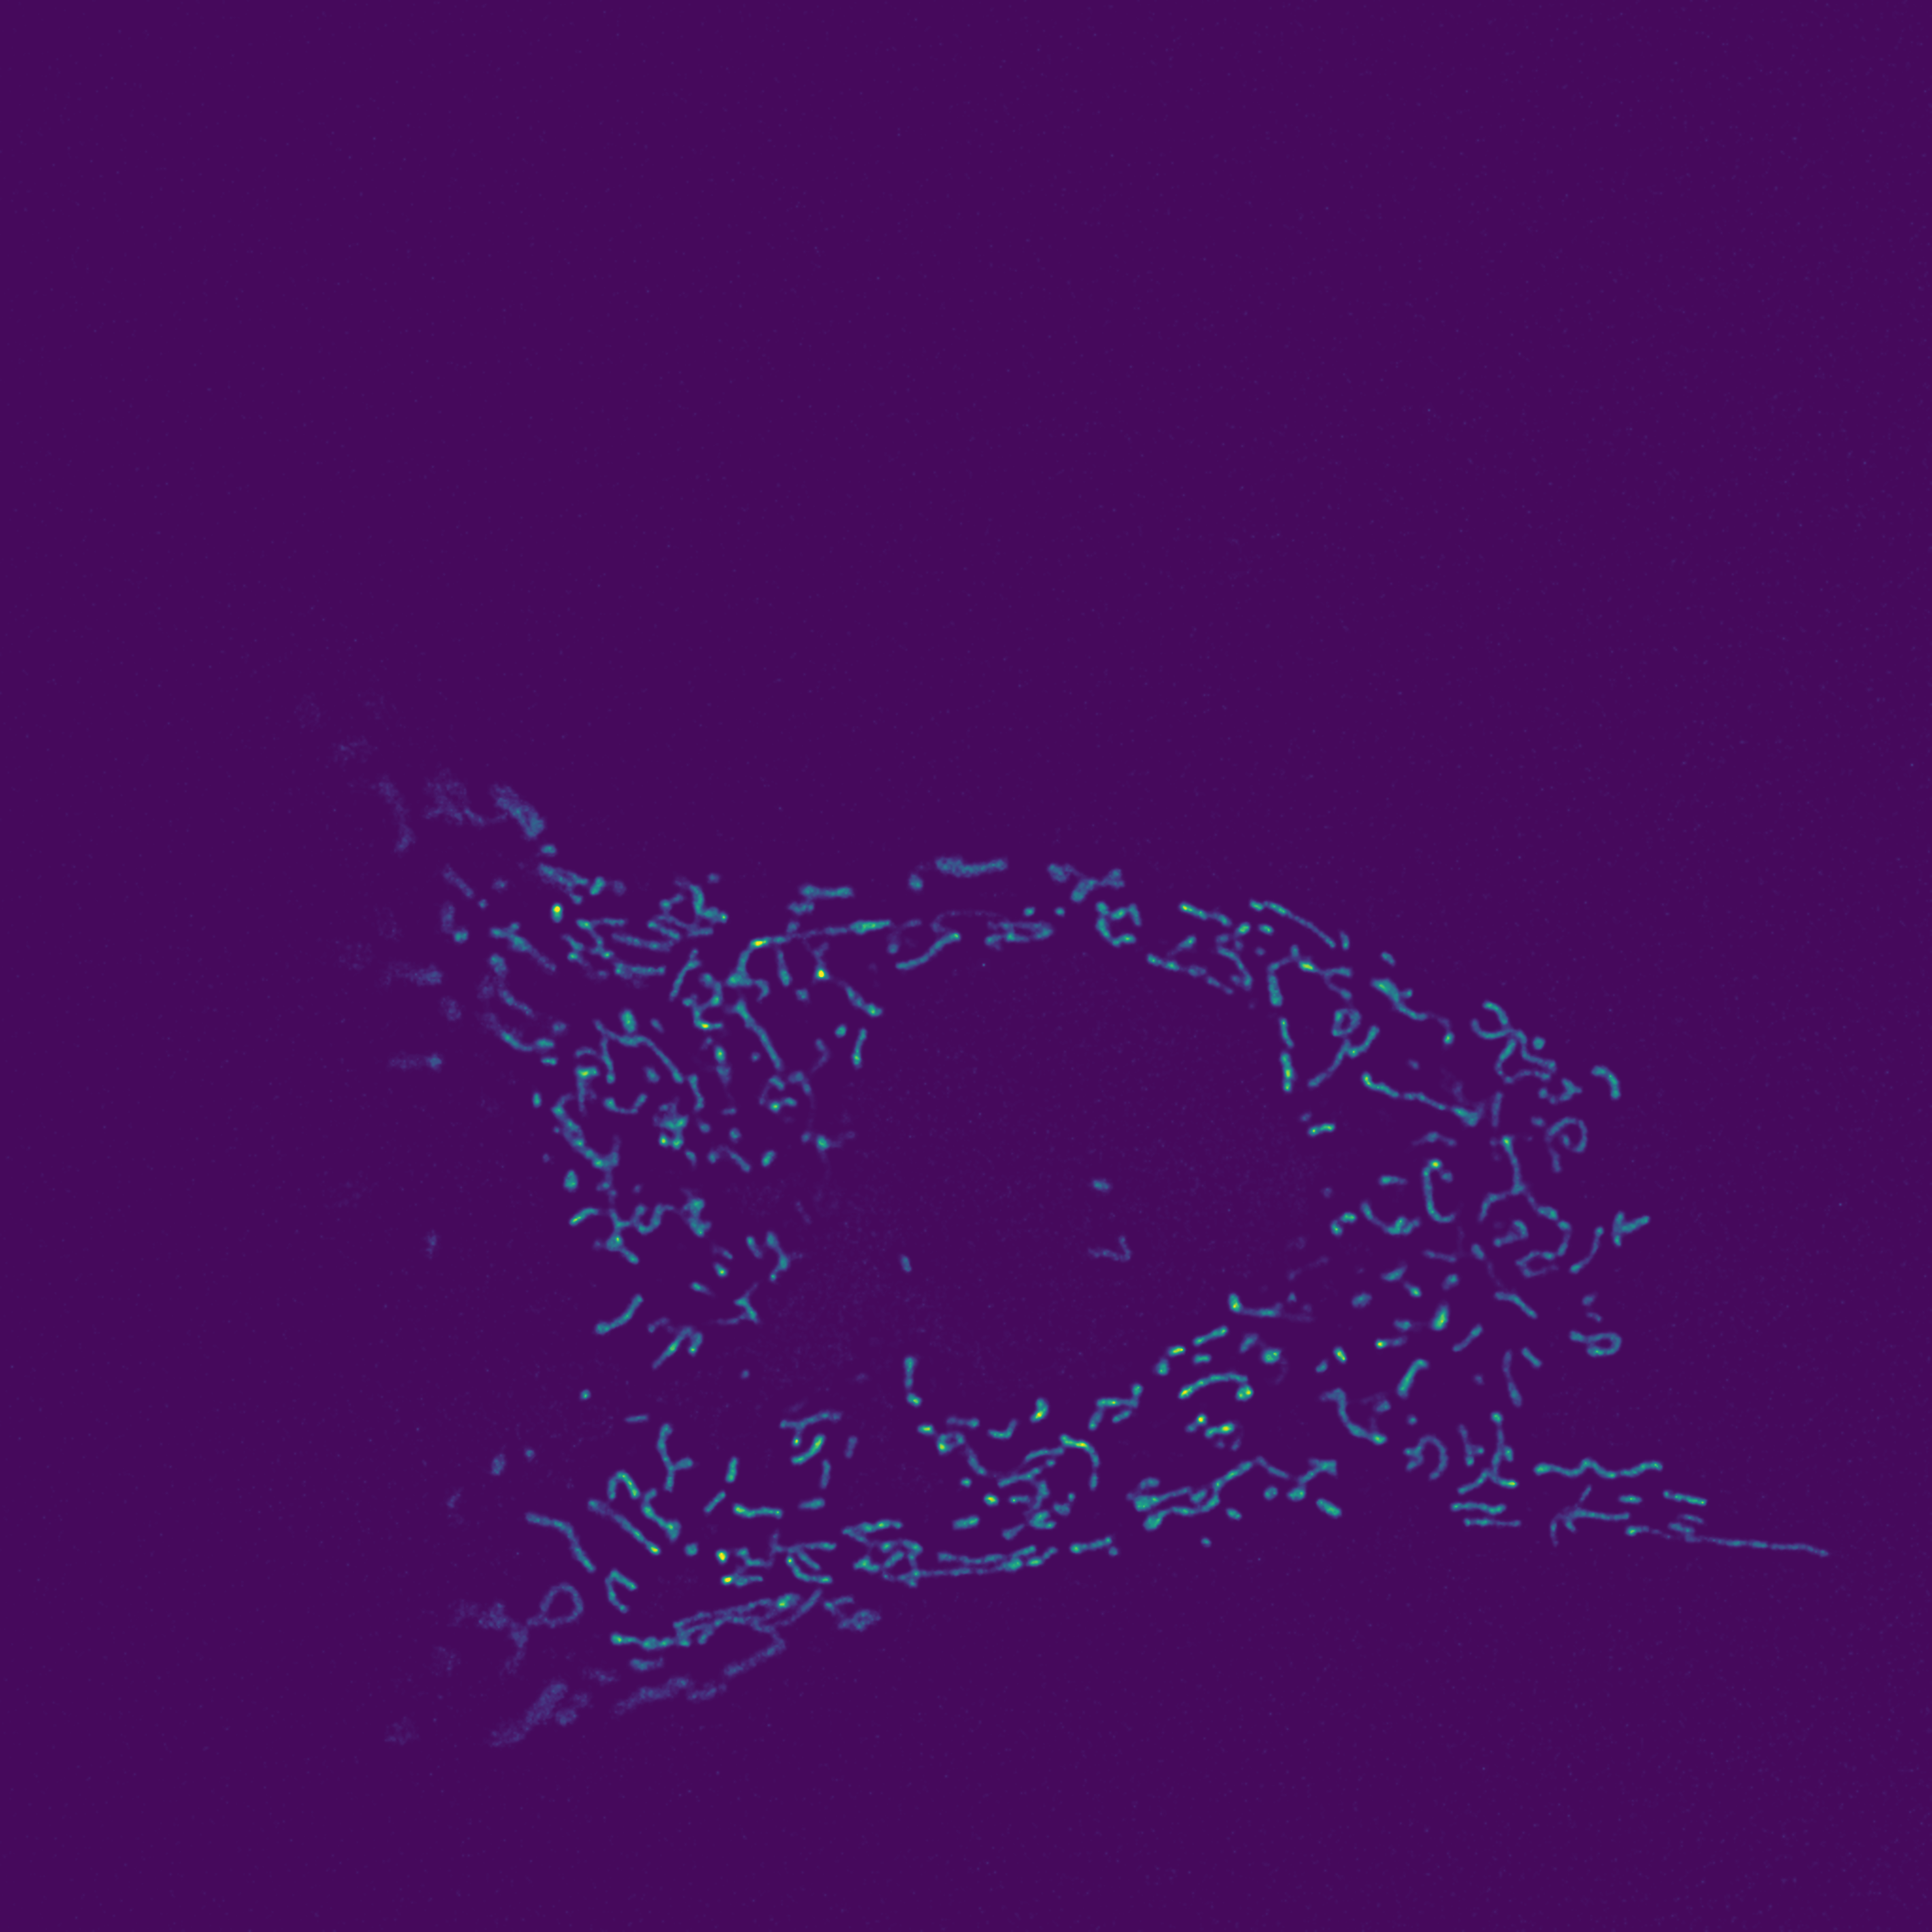
\includegraphics[width=0.49\textwidth]{figs/ch4figs/image_shortlisting/CCCP_1C=1T=0.png}}
	\subcaptionbox{Sample 2 (Lysosomes)}{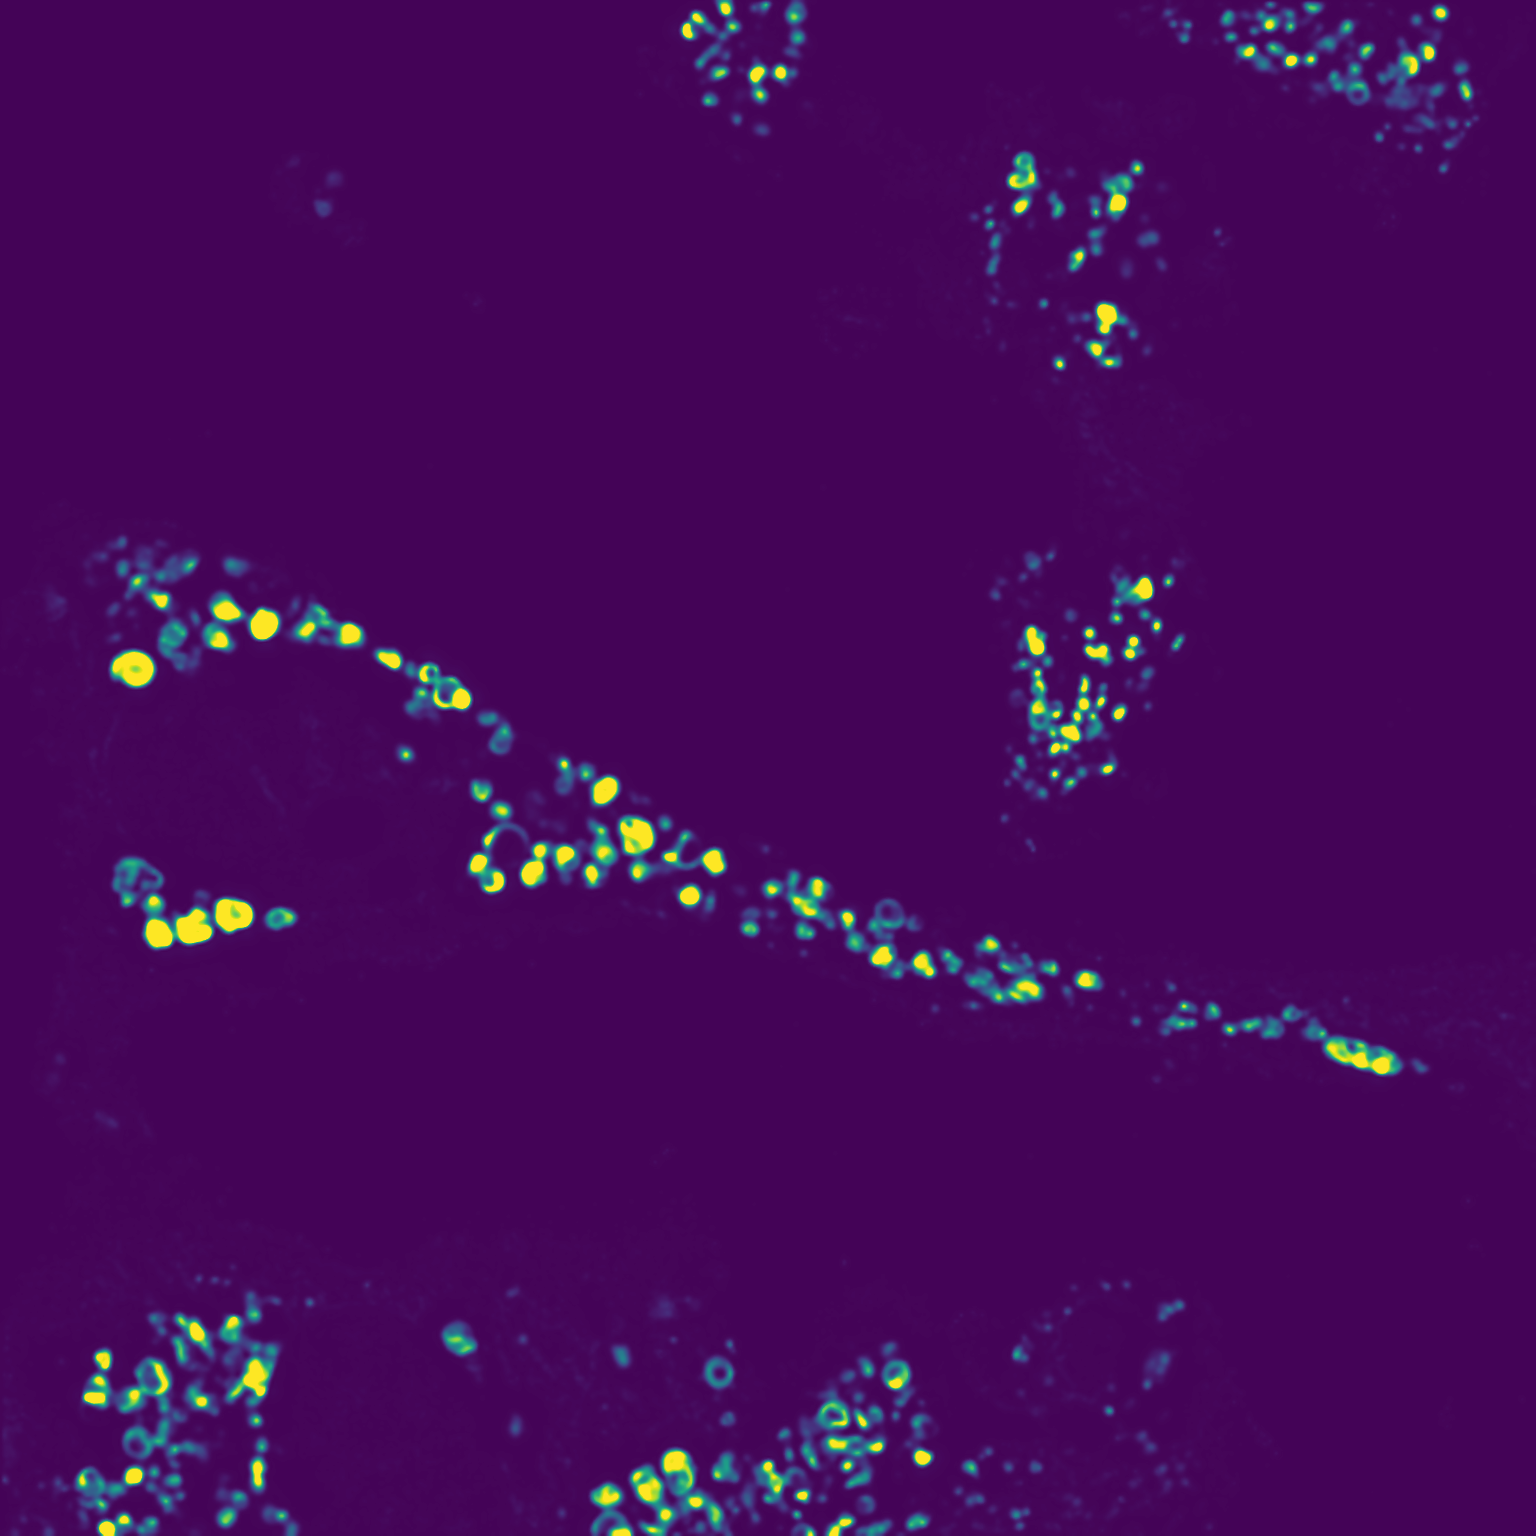
\includegraphics[width=0.49\textwidth]{figs/ch4figs/image_shortlisting/HML_4C=0.png}}
	\subcaptionbox{Sample 3 (Lysosomes)}{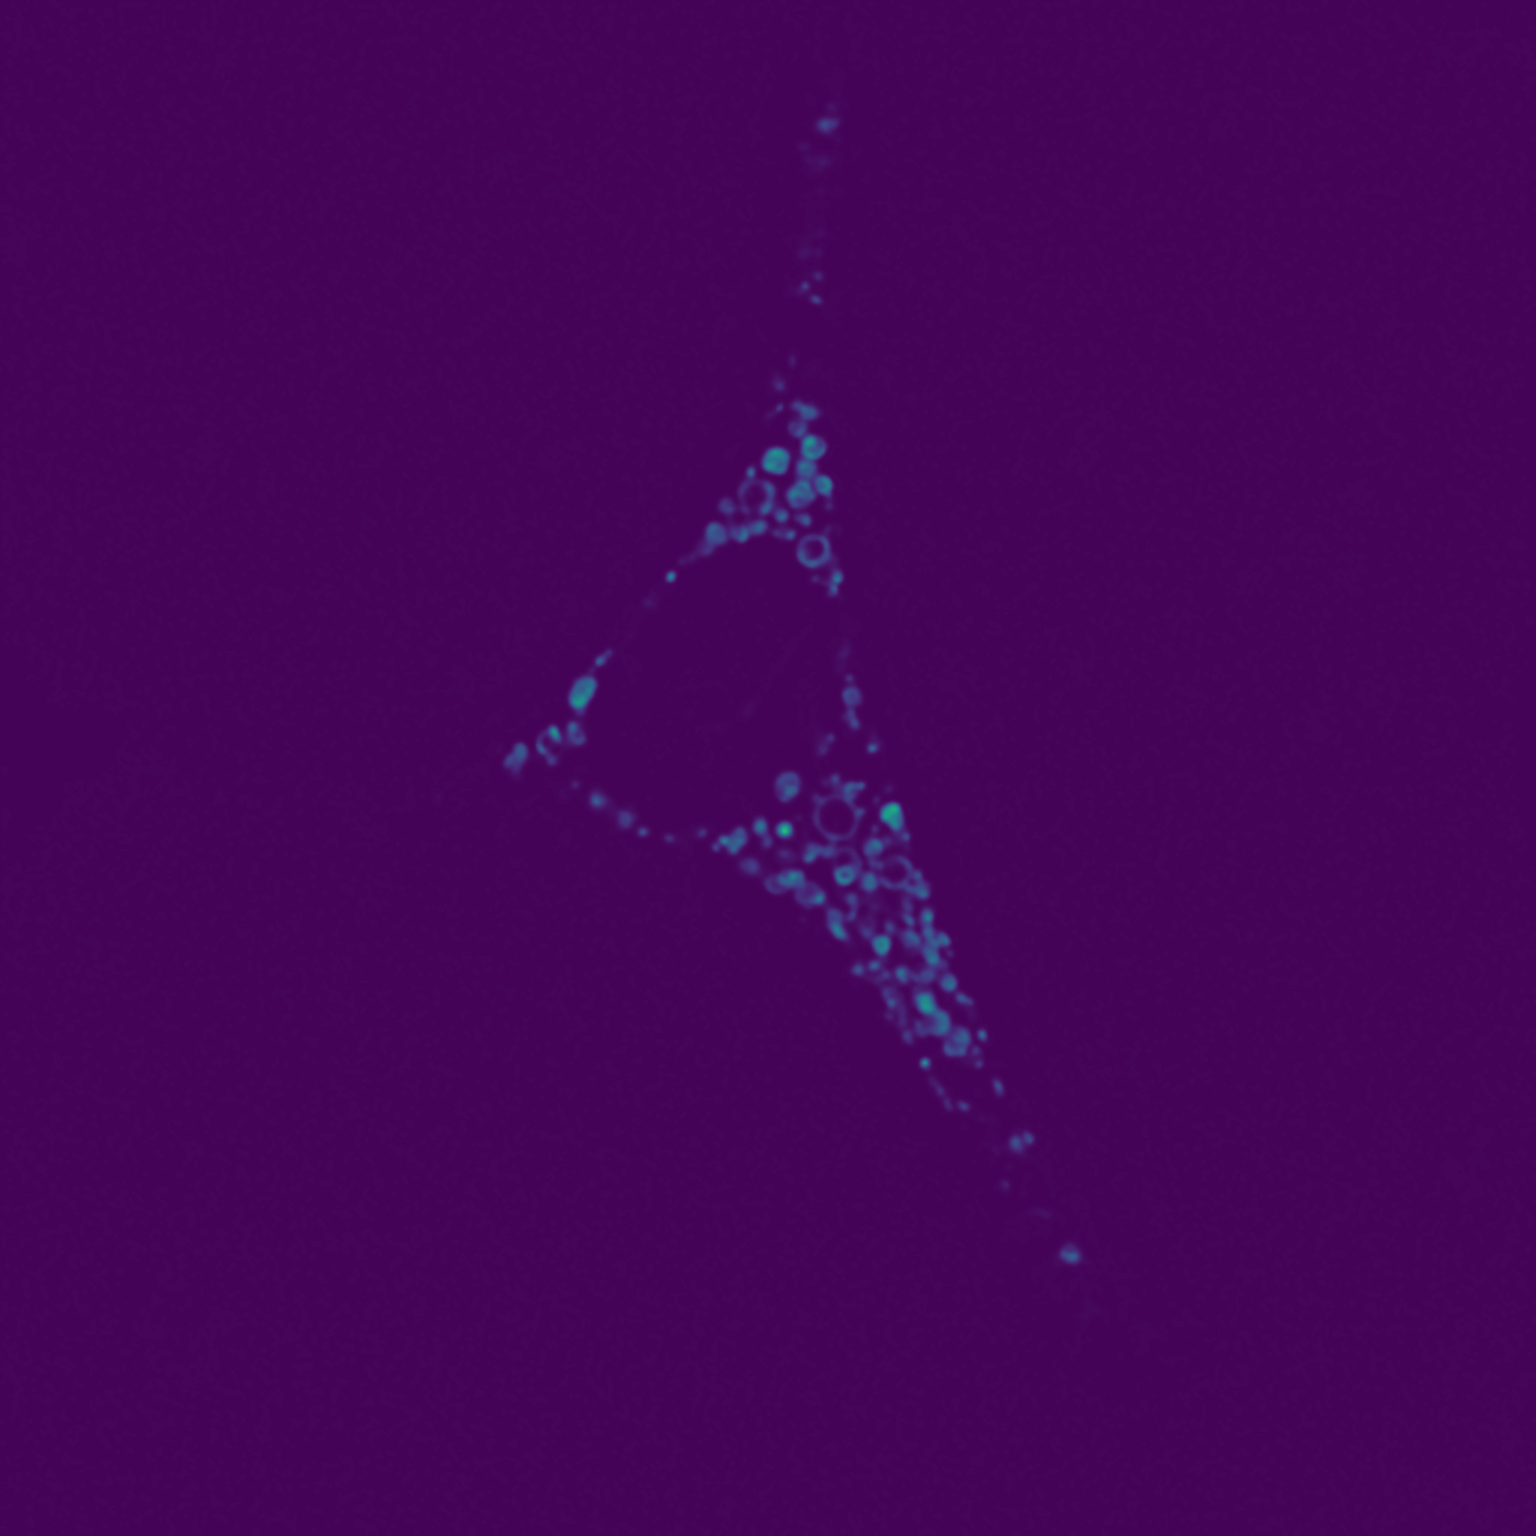
\includegraphics[width=0.49\textwidth]{figs/ch4figs/image_shortlisting/LML_3C=0.png}}
	\subcaptionbox{Sample 4 (Autophagosomes)}{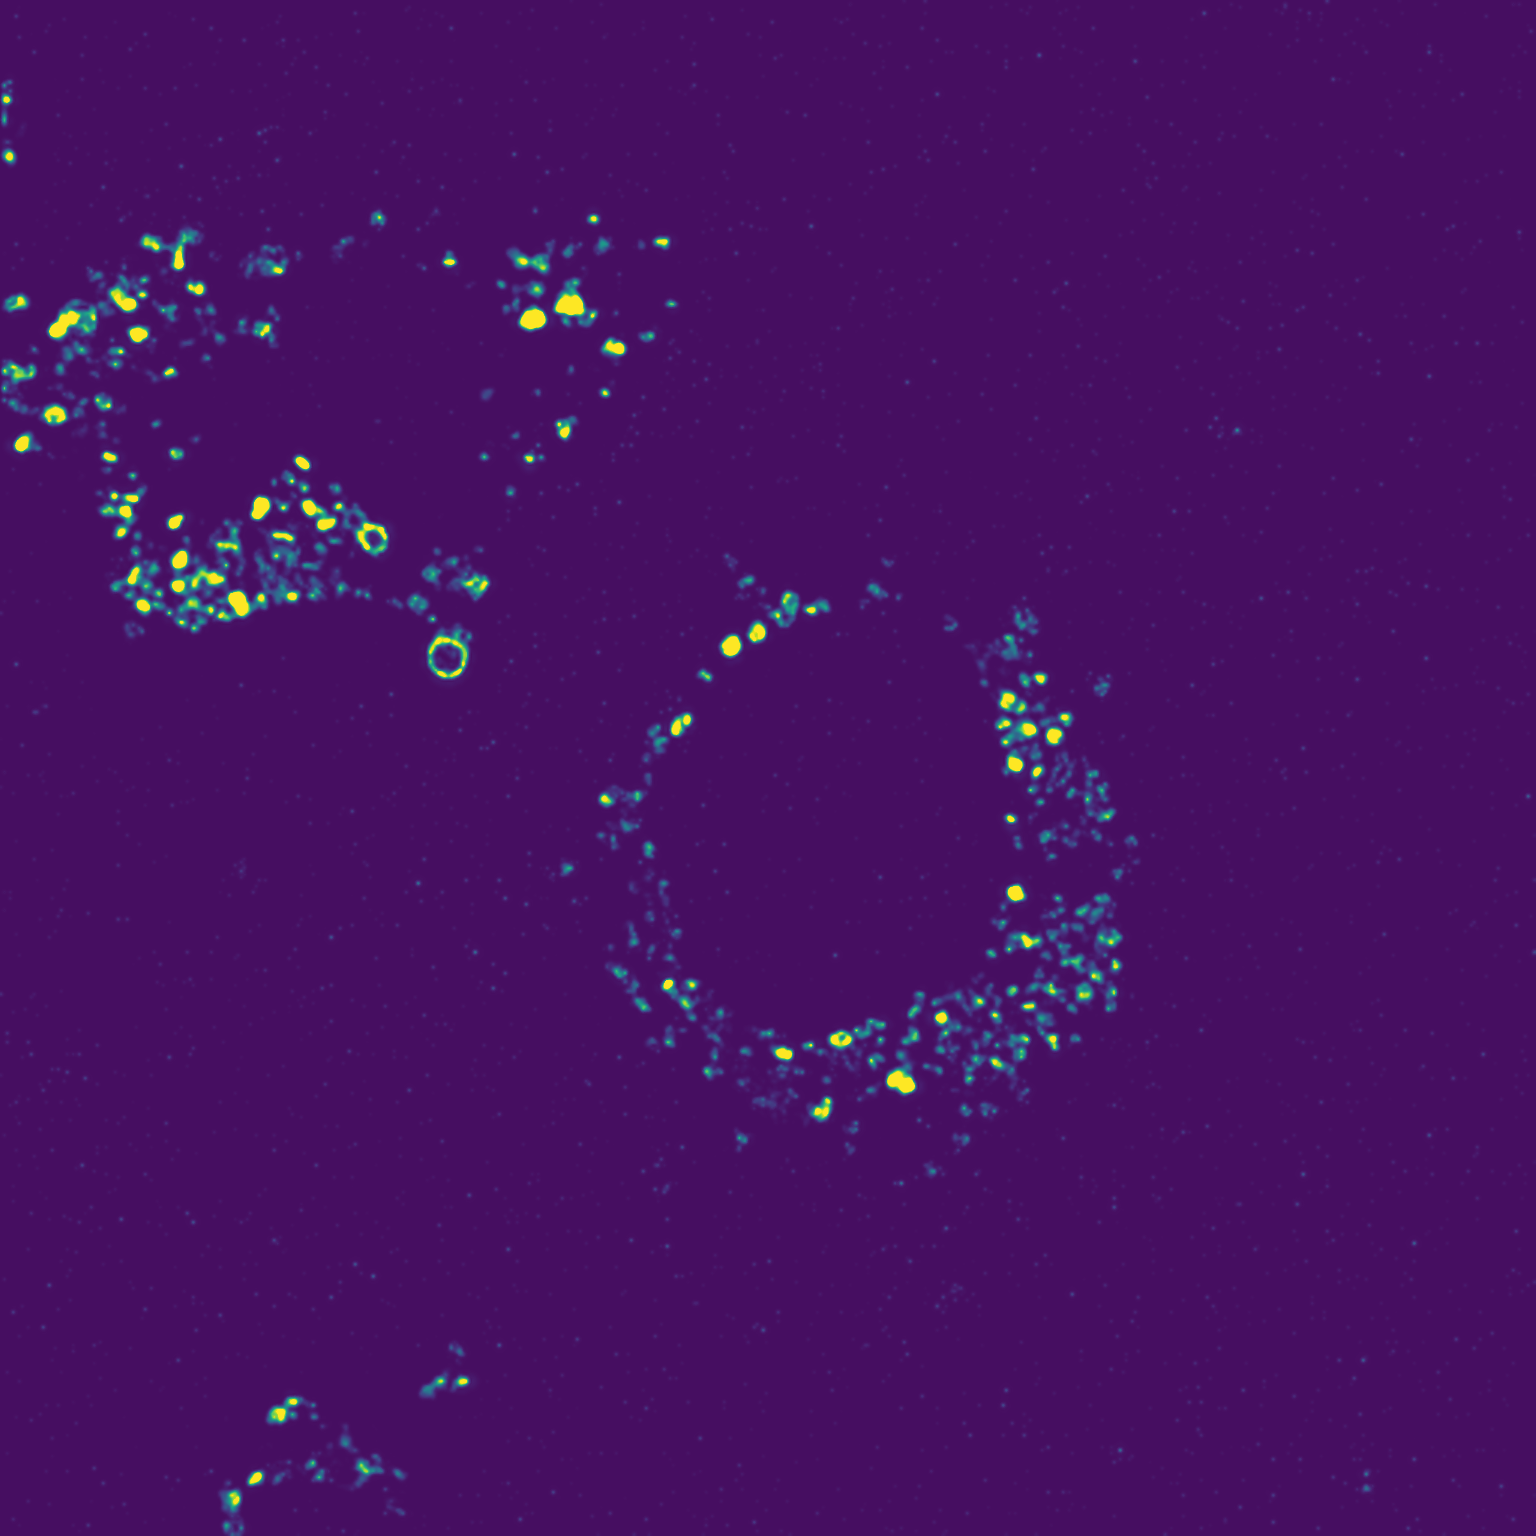
\includegraphics[width=0.49\textwidth]{figs/ch4figs/image_shortlisting/LML_4C=1.png}}
	\caption[Set of samples used to shortlist the threshold methods.]{Set of samples used to shortlist the threshold methods. The centre slice of the images, rounded down where necessary, of the images is shown.}
	\label{fig:shortlist_raw}
\end{figure}

\begin{figure}[ht!]
	\centering
	\subcaptionbox{Original sample image B\label{subfig:og_C_badthresh}}{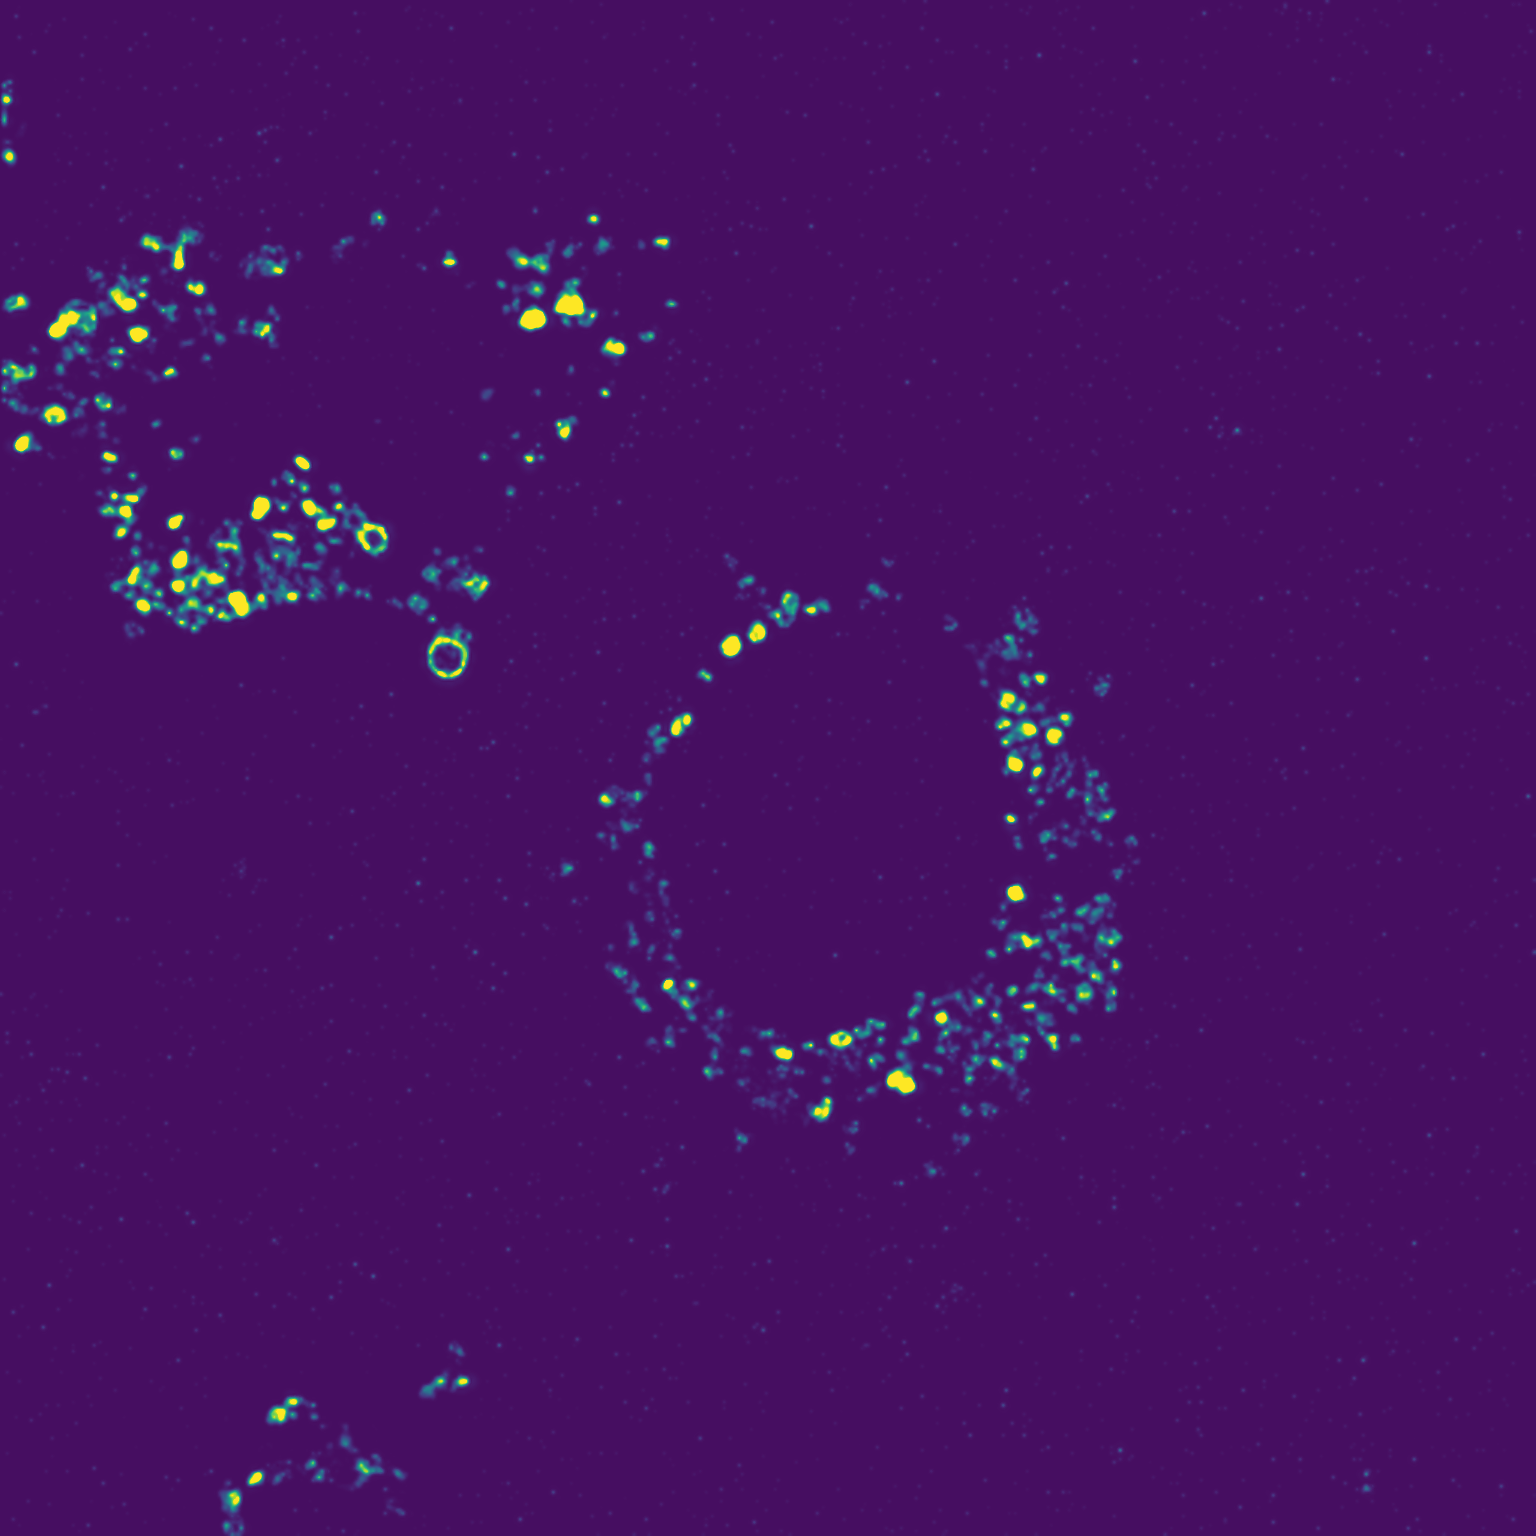
\includegraphics[width=0.45\textwidth]{figs/ch4figs/image_shortlisting/LML_4C=1.png}}
	\subcaptionbox{Original sample image C\label{subfig:og_B_badthresh}}{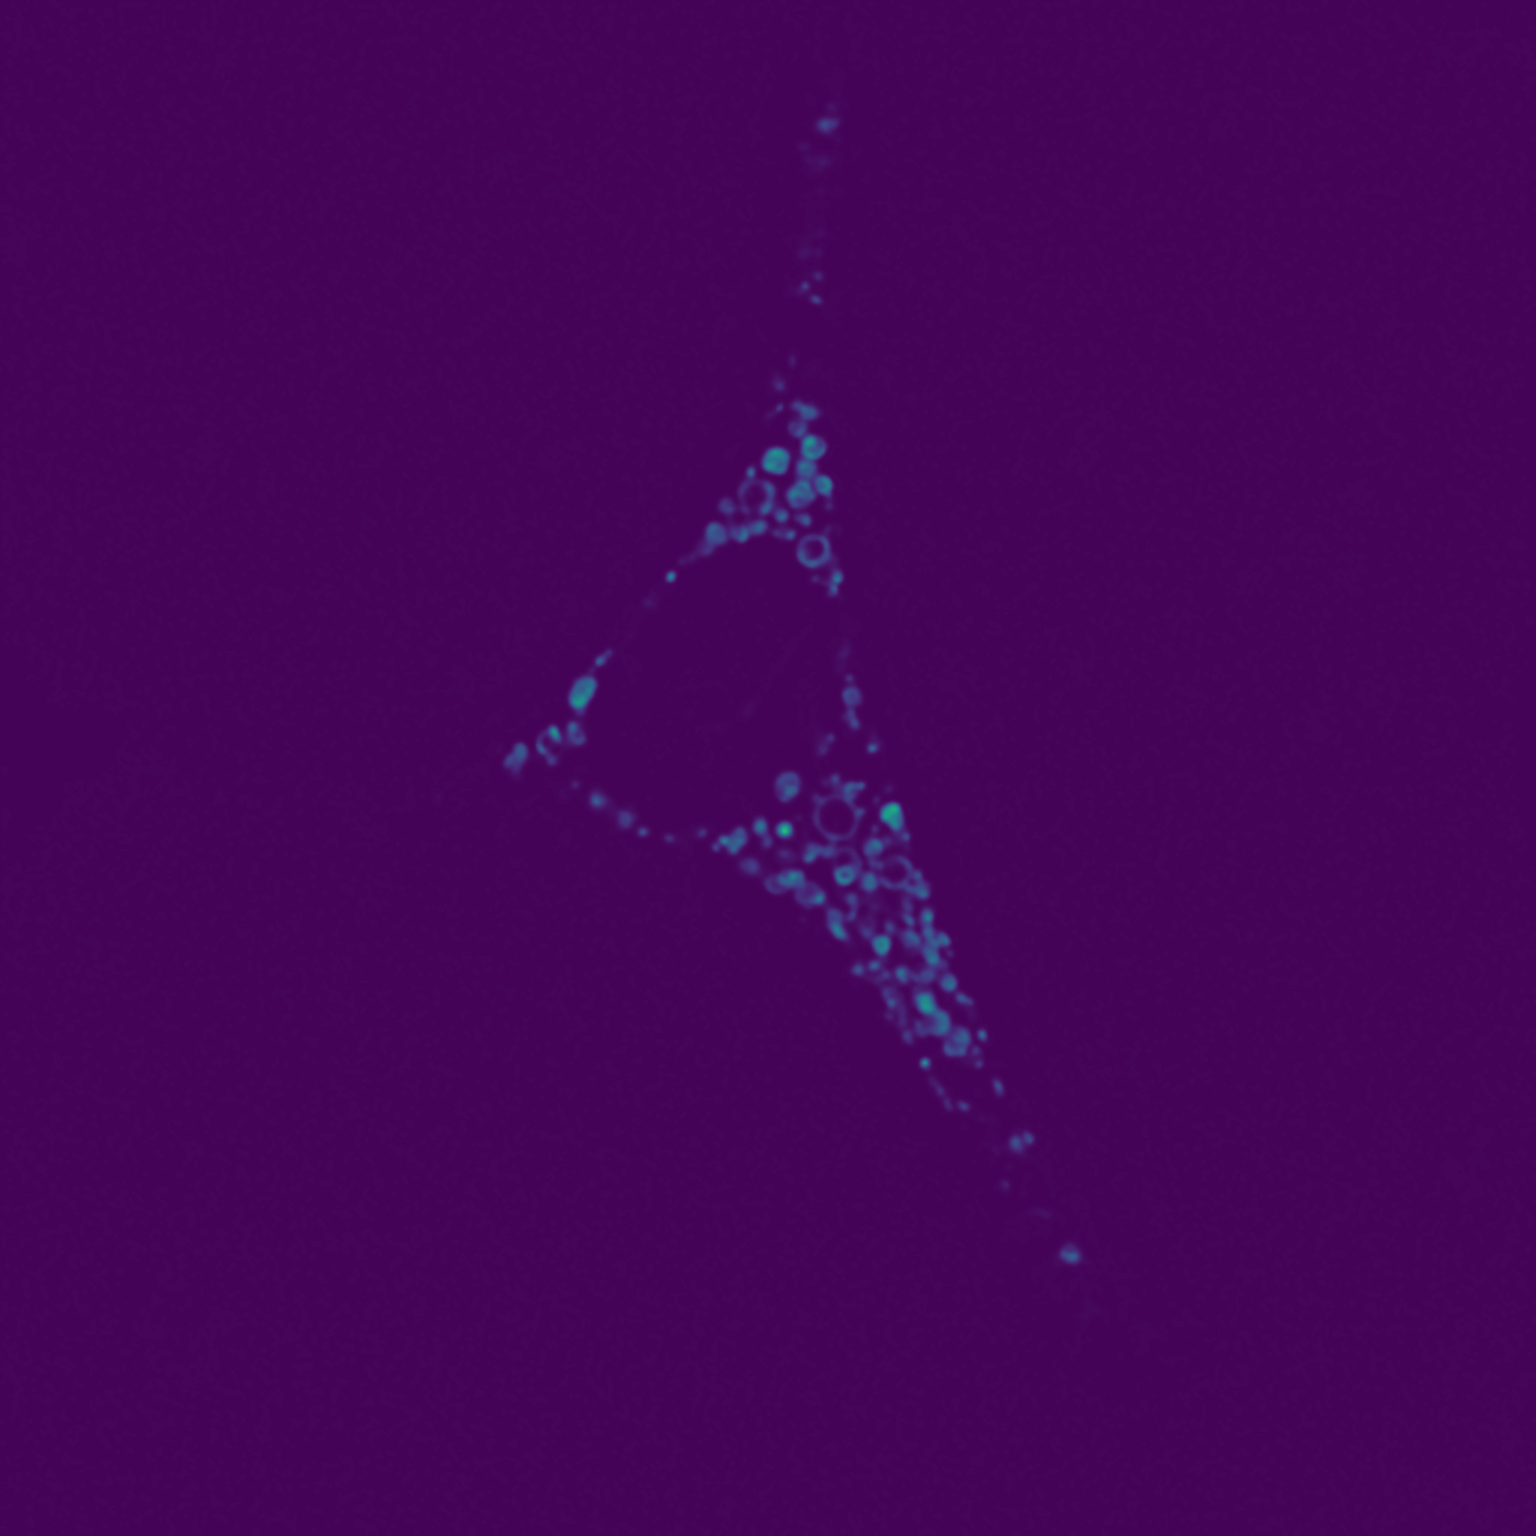
\includegraphics[width=0.45\textwidth]{figs/ch4figs/image_shortlisting/LML_3C=0.png}}
	\subcaptionbox{Mild background inclusion\label{subfig:mild_inclusion_C}}{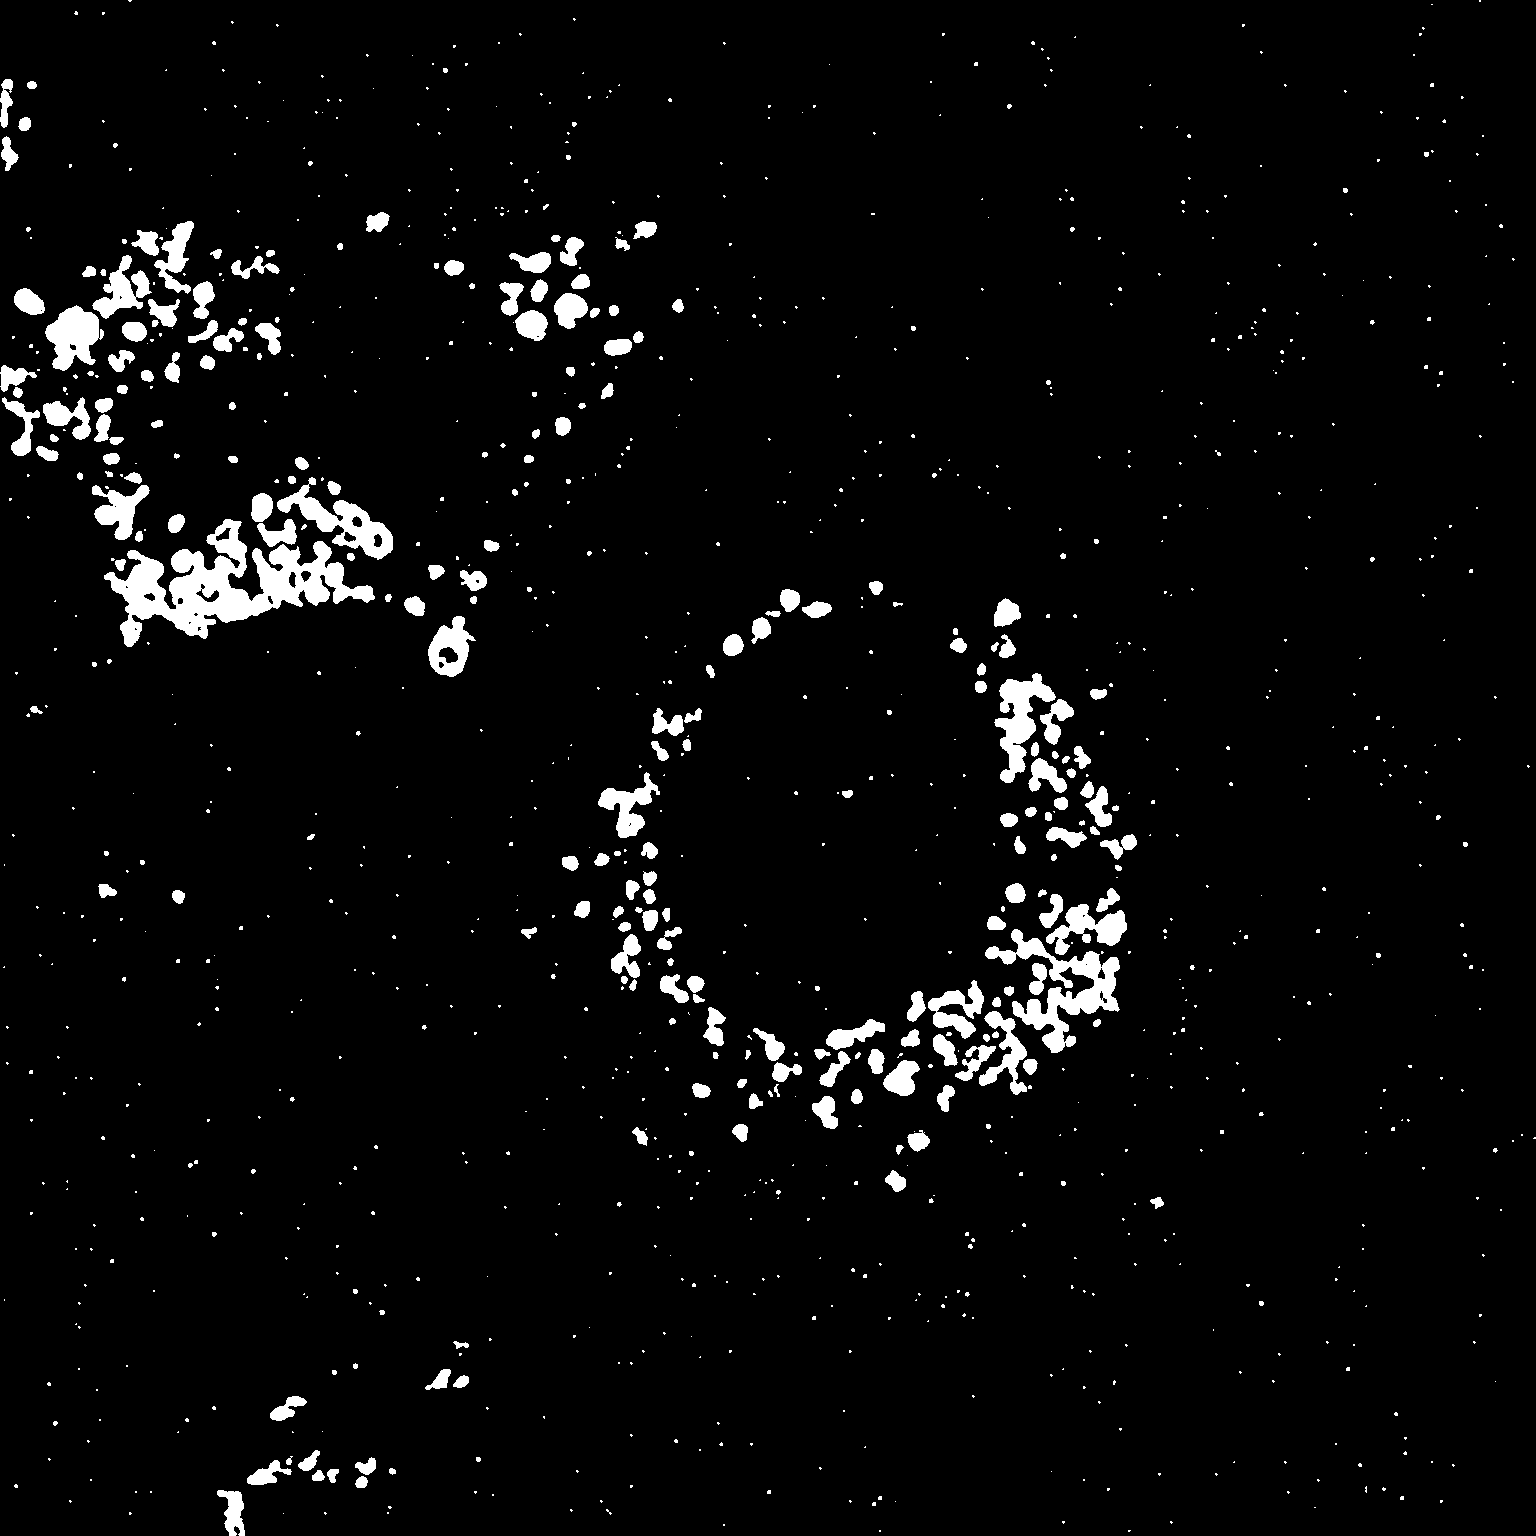
\includegraphics[width=0.45\textwidth]{figs/ch4figs/image_shortlisting/global/Li_LML_4C=1.png}}
	\subcaptionbox{Major background inclusion\label{subfig:major_inclusion_B}}{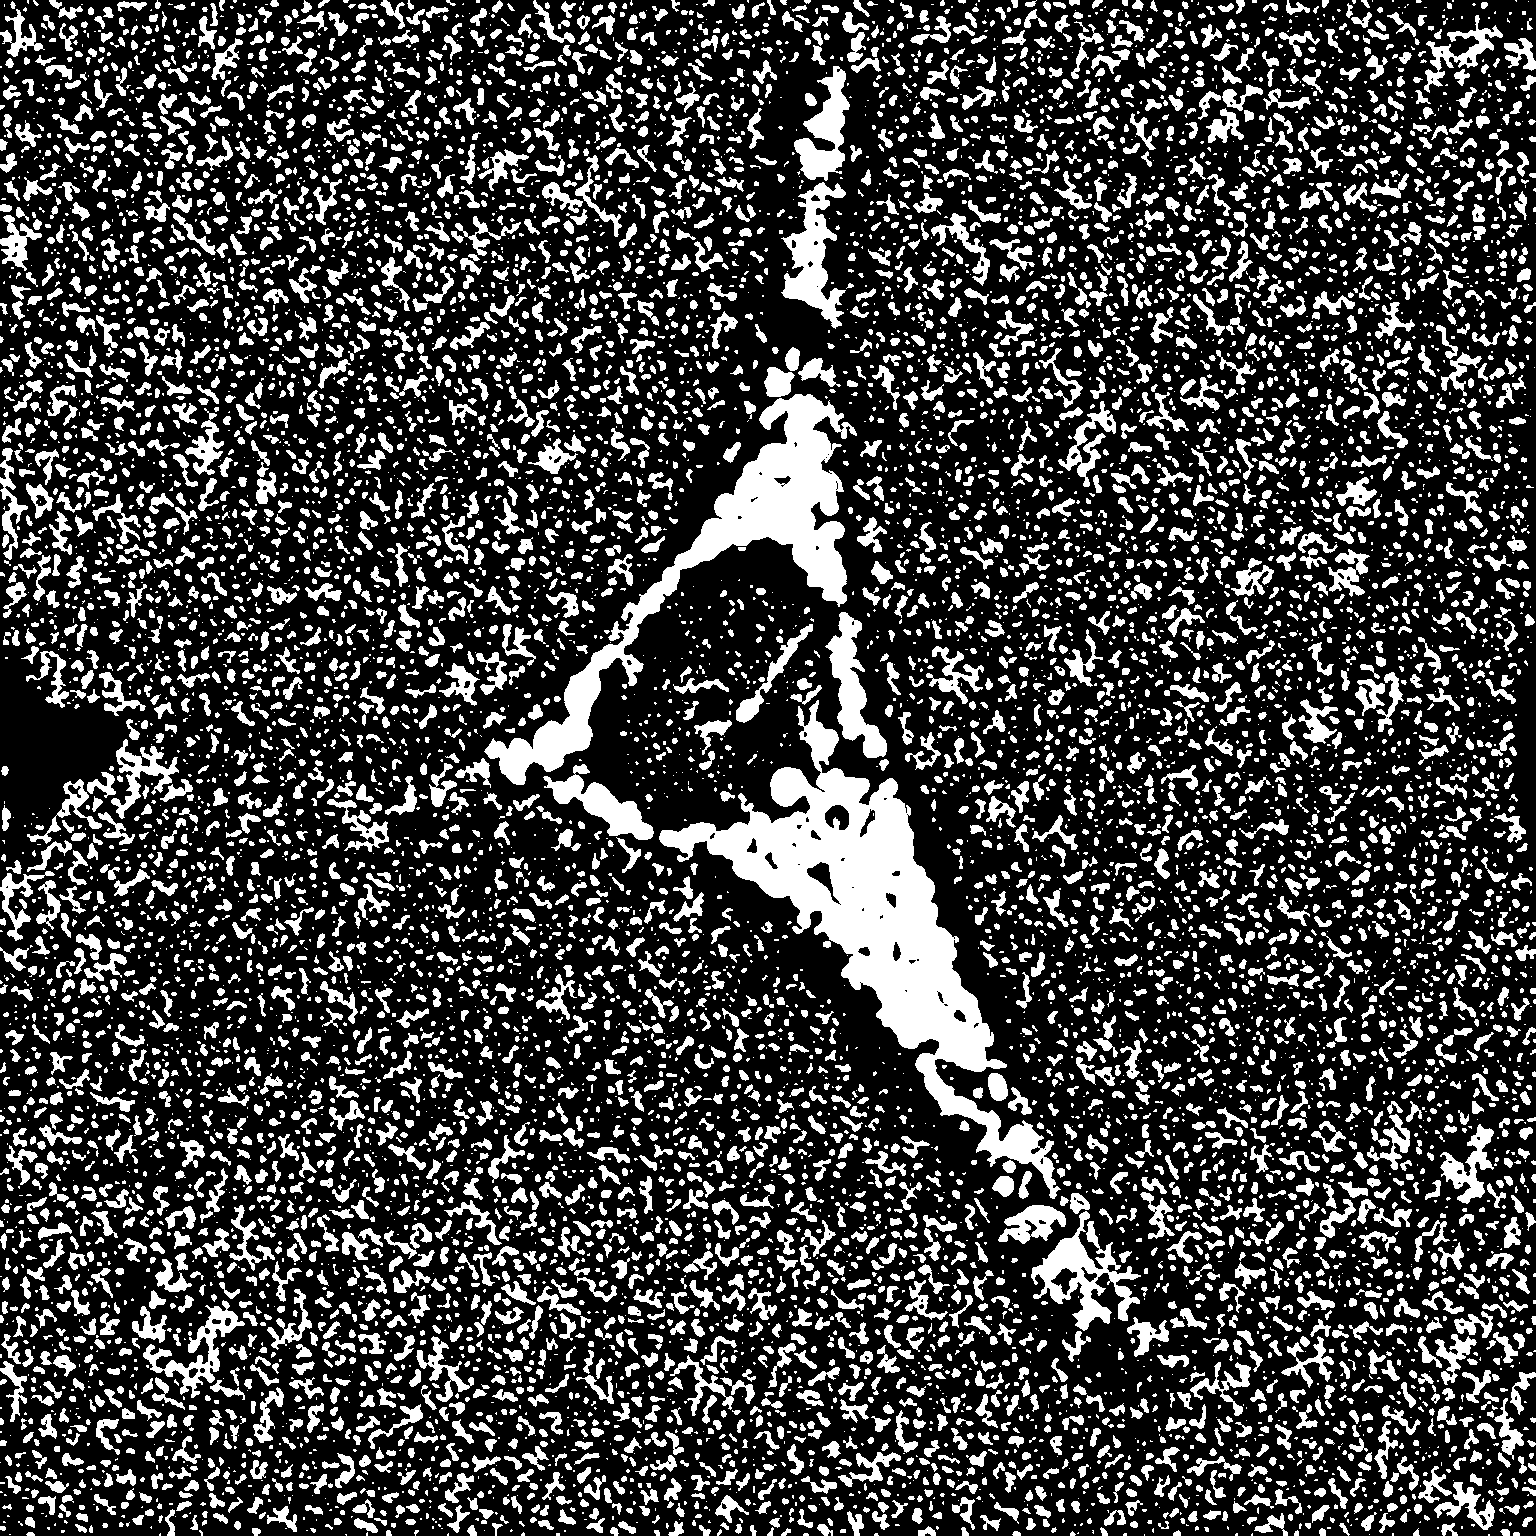
\includegraphics[width=0.45\textwidth]{figs/ch4figs/image_shortlisting/global/Mean_LML_3C=0.png}}
	\subcaptionbox{Mild foreground exclusion\label{subfig:mild_exclusion_C}}{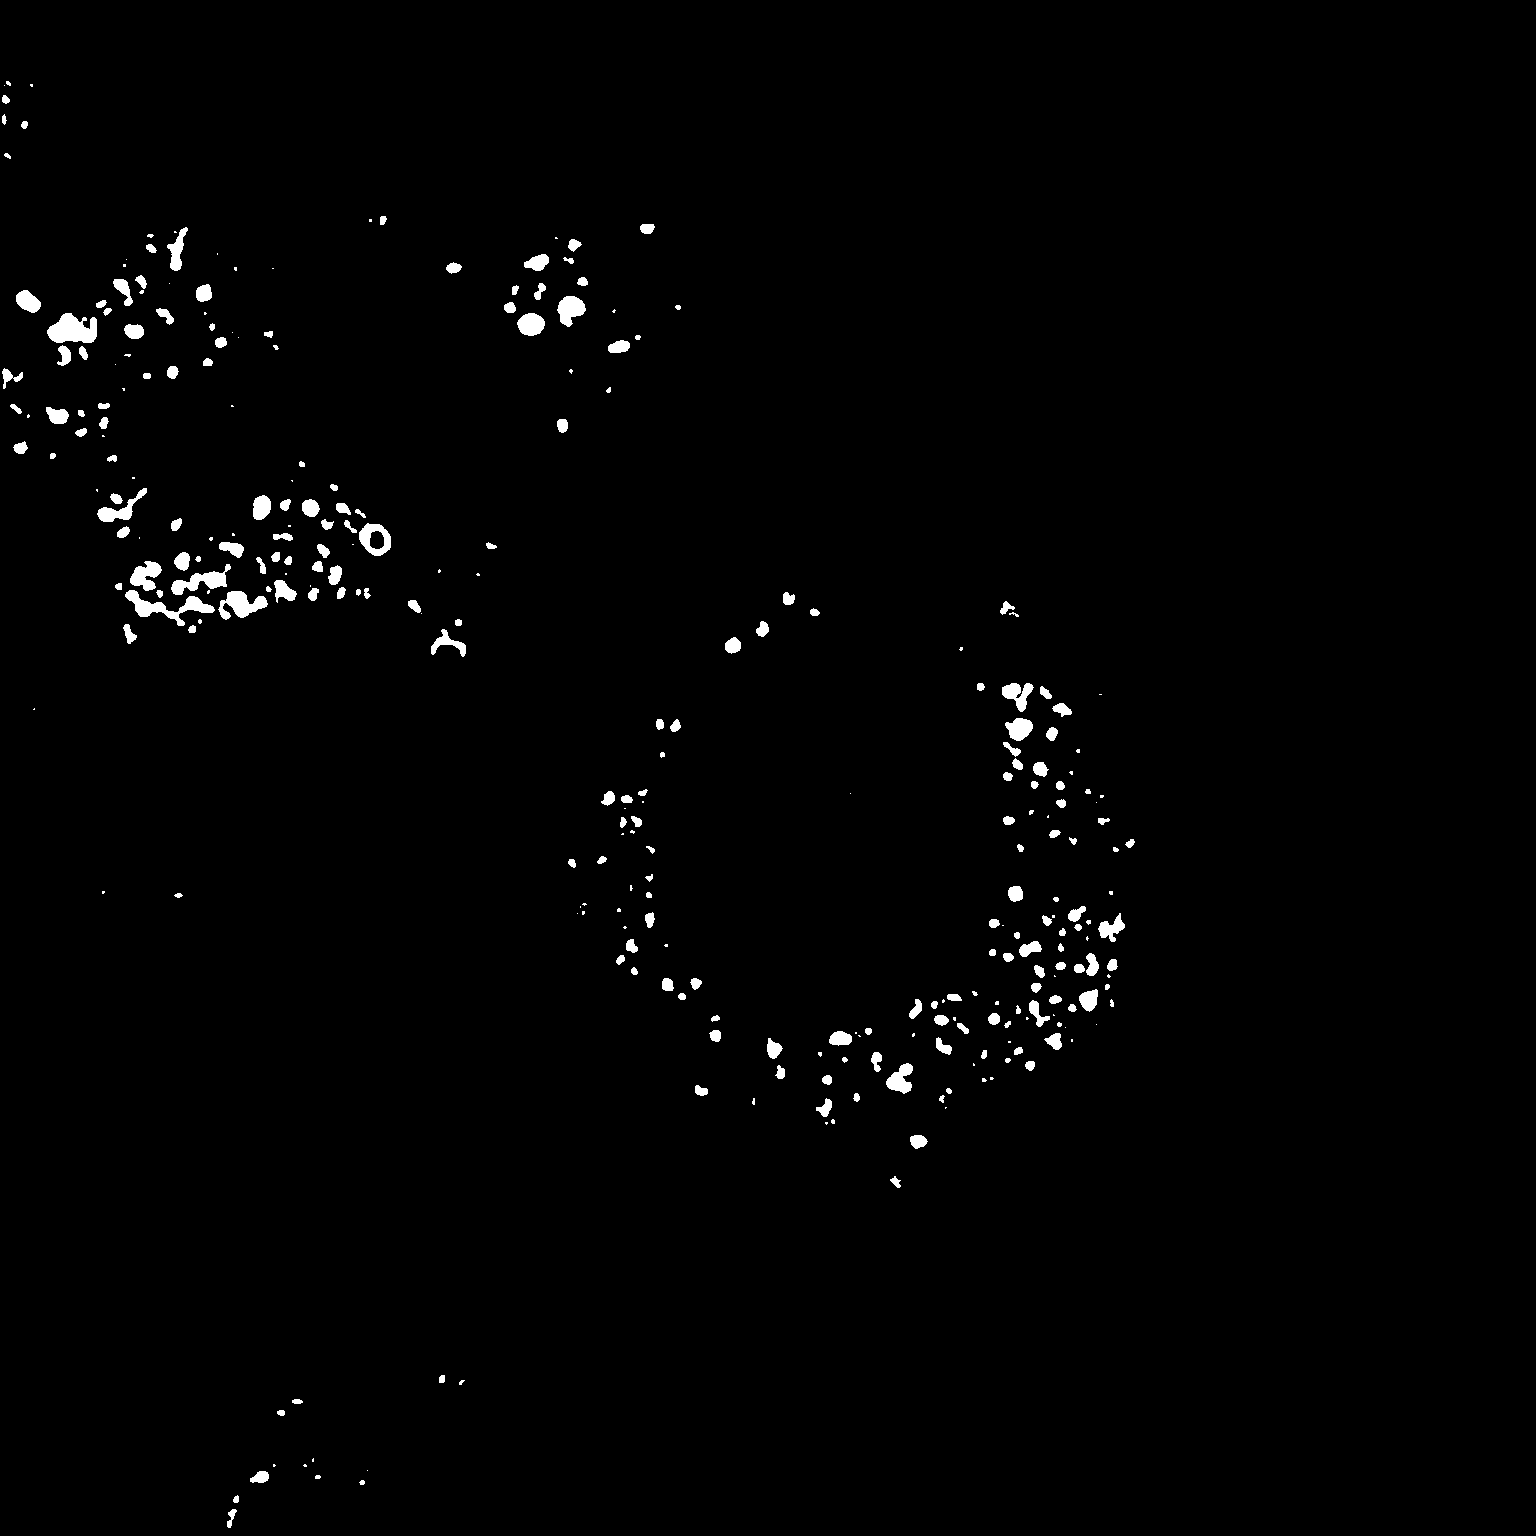
\includegraphics[width=0.45\textwidth]{figs/ch4figs/image_shortlisting/global/Moments_LML_4C=1.png}}
	\subcaptionbox{Major foreground exclusion\label{subfig:major_exclusion_B}}{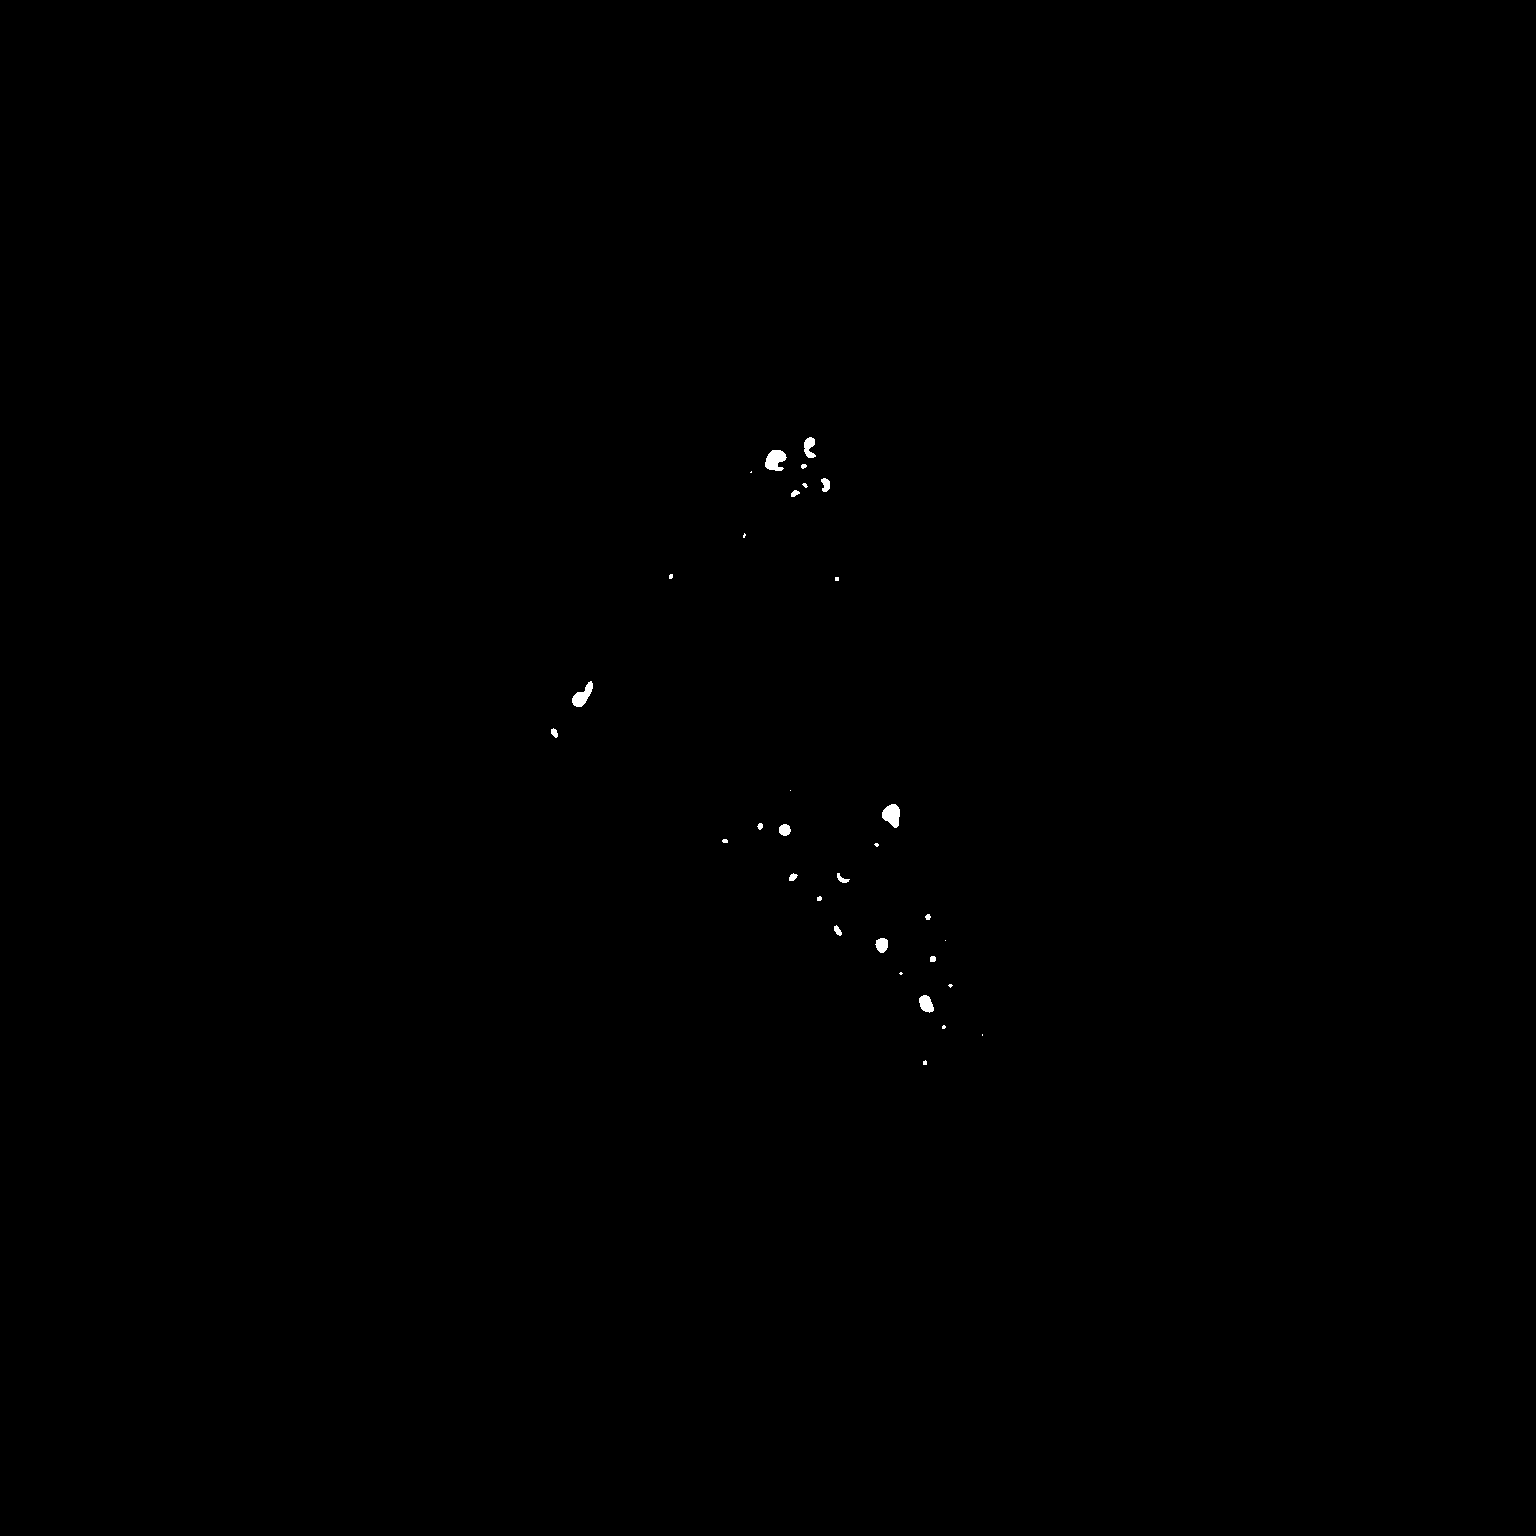
\includegraphics[width=0.45\textwidth]{figs/ch4figs/image_shortlisting/global/Intermodes_LML_3C=0.png}}
	\caption[Examples of both mild and major cases of background inclusion and foreground exclusion.]{Examples of both mild and major cases of background inclusion and of foreground exclusion. The sample images presented are Samples 2 and 3, shown in \ref{fig:shortlist_raw}, with (\subref{subfig:og_B_badthresh}), (\subref{subfig:major_inclusion_B}), and (\subref{subfig:major_exclusion_B}) representing the former and (\subref{subfig:og_C_badthresh}), (\subref{subfig:mild_inclusion_C}), and (\subref{subfig:mild_exclusion_C}) representing the latter.}
	\label{fig:bad_threshes_shortlist}
\end{figure}


\clearpage
\subsection{Global threshold shortlisting} 
A total of 16 global threshold methods, provided by the \textit{Auto Threshold} plugin, were tested across the shortlisting sample set:
\begin{multicols}{4}
	\begin{itemize}
		\setlength\itemsep{1mm}
		\item Huang
		\item Huang2
		\item Intermodes
		\item IsoData
		\item Li
		\item MaxEntropy
		\item Mean
		\item MinError(I)
		\item Minimum
		\item Moments
		\item Otsu
		\item Percentile
		\item RenyiEntropy
		\item Shanbhag
		\item Triangle
		\item Yen
	\end{itemize}
\end{multicols}
\paragraph{Findings:} Of the global thresholding methods explored, the Huang2, IsoData, Li, MaxEntropy, Moments, Otsu, RenyiEntropy, Triangle, and Yen methods were deemed viable for further evaluation due to the presence of mostly mild foreground exclusion and background inclusion and it is nuanced whether mild cases are detrimental and, if so, to what degree. While evaluating the severity of these is subjective, save for the extreme cases, it was observed that the viable methods only present at most two mild cases per method while only the Triangle method presents a singular instance of more severe background inclusion although this is still not comparable to the major case illustrated in Figure \ref{fig:bad_threshes_shortlist} (\subref{subfig:major_inclusion_B}). While this does not imply that the performance of these methods will be the same for evaluations involving different image data sets, it does flag methods expressing major foreground exclusion and background inclusion behaviours. Major occurrences of background inclusion can be seen in methods Huang (Figure \ref{append-fig:huang_short}), Mean (Figure \ref{append-fig:Mean_short}), MinError(I) (Figure \ref{append-fig:MinError_short}), and Percentile (Figure \ref{append-fig:Percentile_short}) while major occurrences of foreground exclusion can be seen in methods Intermodes (Figure \ref{append-fig:Intermodes_short}), Minimum (Figure \ref{append-fig:Minimum_short}), and Shanbhag (Figure \ref{append-fig:Shanbhag_short}). Due to this, these methods have been deemed not worth further exploration in this study due to this poor performance and the showcasing of a singular case of either major foreground exclusion or background inclusion, dependent on the method, is shown in Figure \ref{fig:bad_global_subset} for the methods not deemed worth further exploration. 

\begin{figure}[ht!]
	\centering
	\subcaptionbox{Intermodes applied to Sample 4}{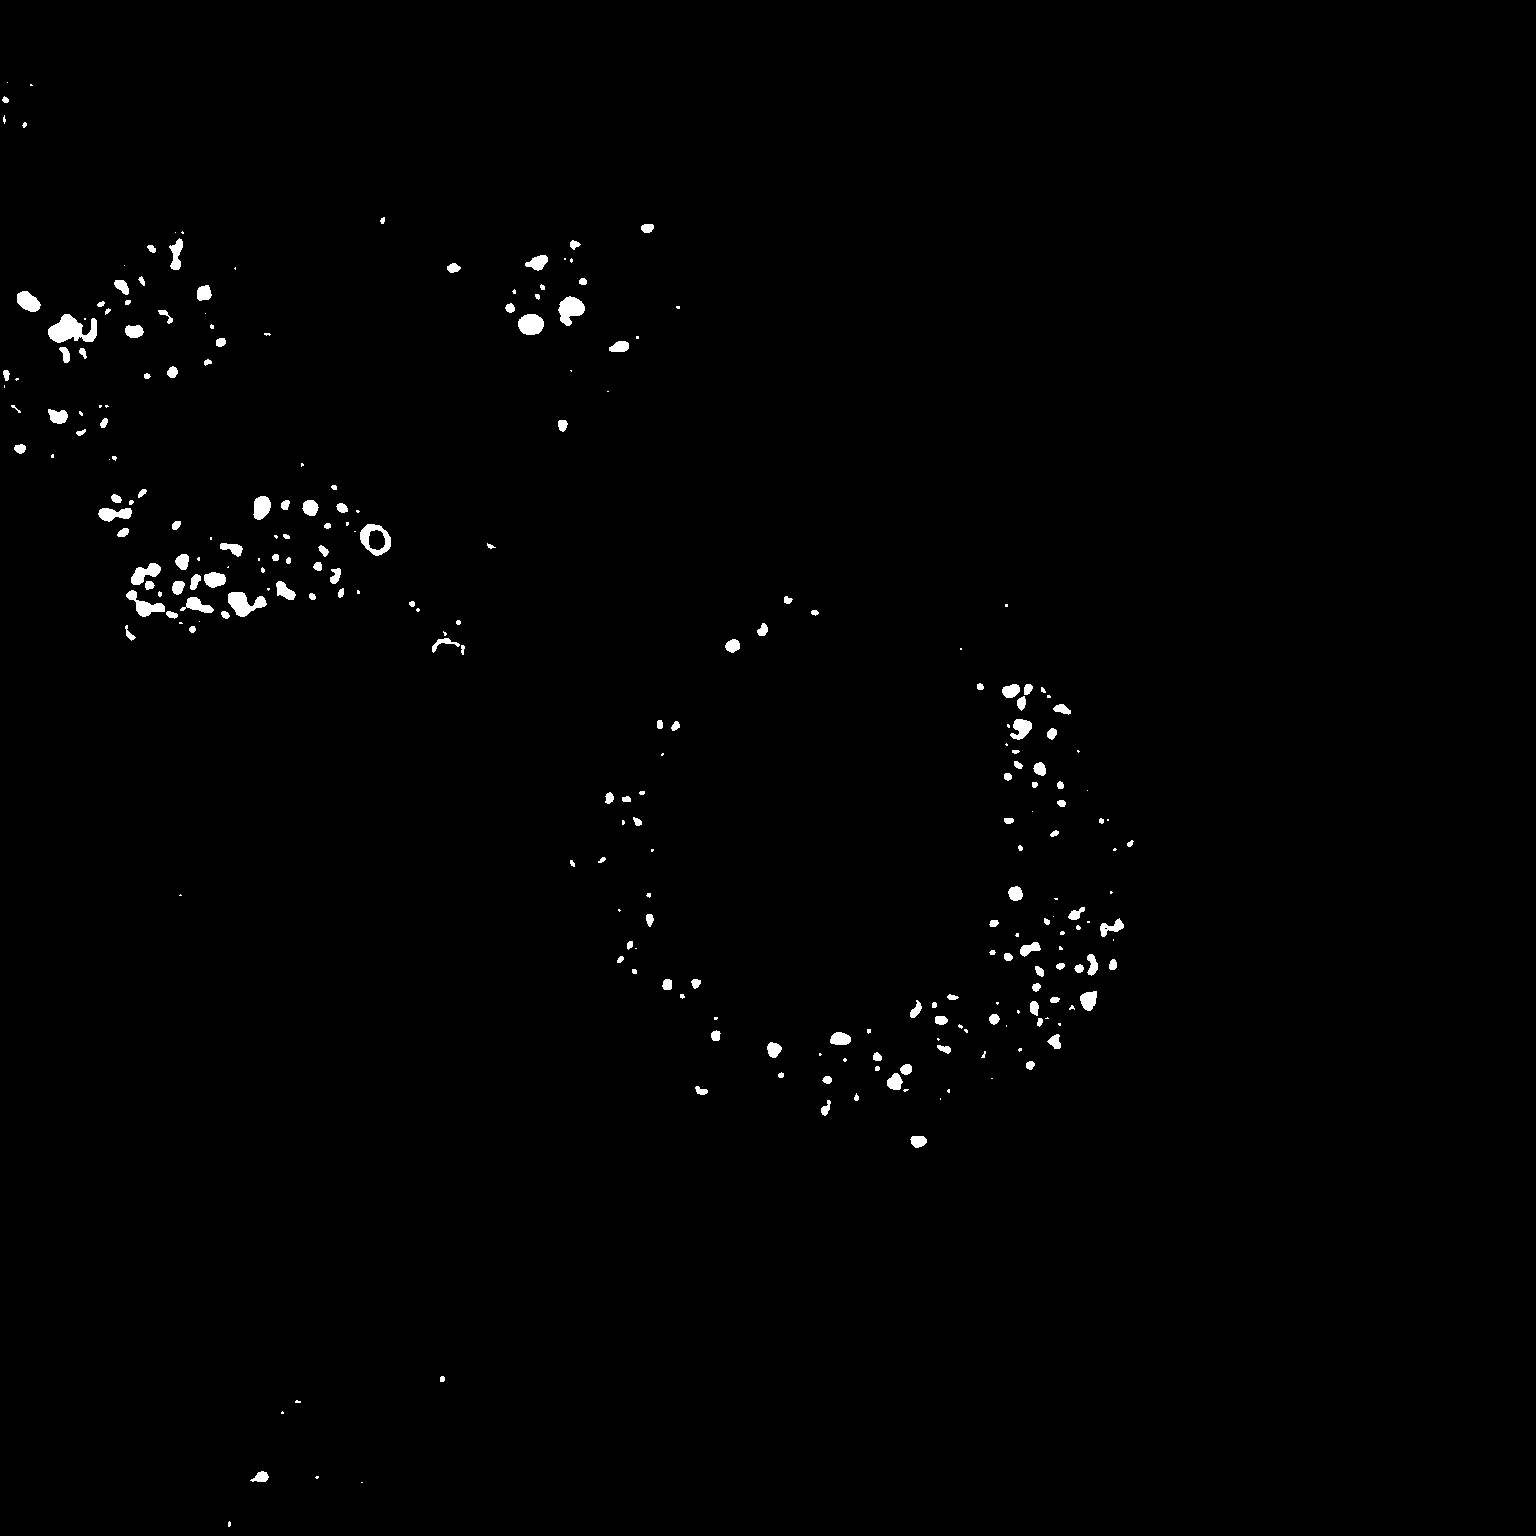
\includegraphics[width=0.24\textwidth]{figs/ch4figs/image_shortlisting/global/Intermodes_LML_4C=1.png}}
	\subcaptionbox{Minimum applied to Sample 1}{
\includegraphics[width=0.24\textwidth]{figs/ch4figs/image_shortlisting/global/Minimum_CCCP_1C=1T=0.png}}
	\subcaptionbox{Shanbhag applied to Sample 4}{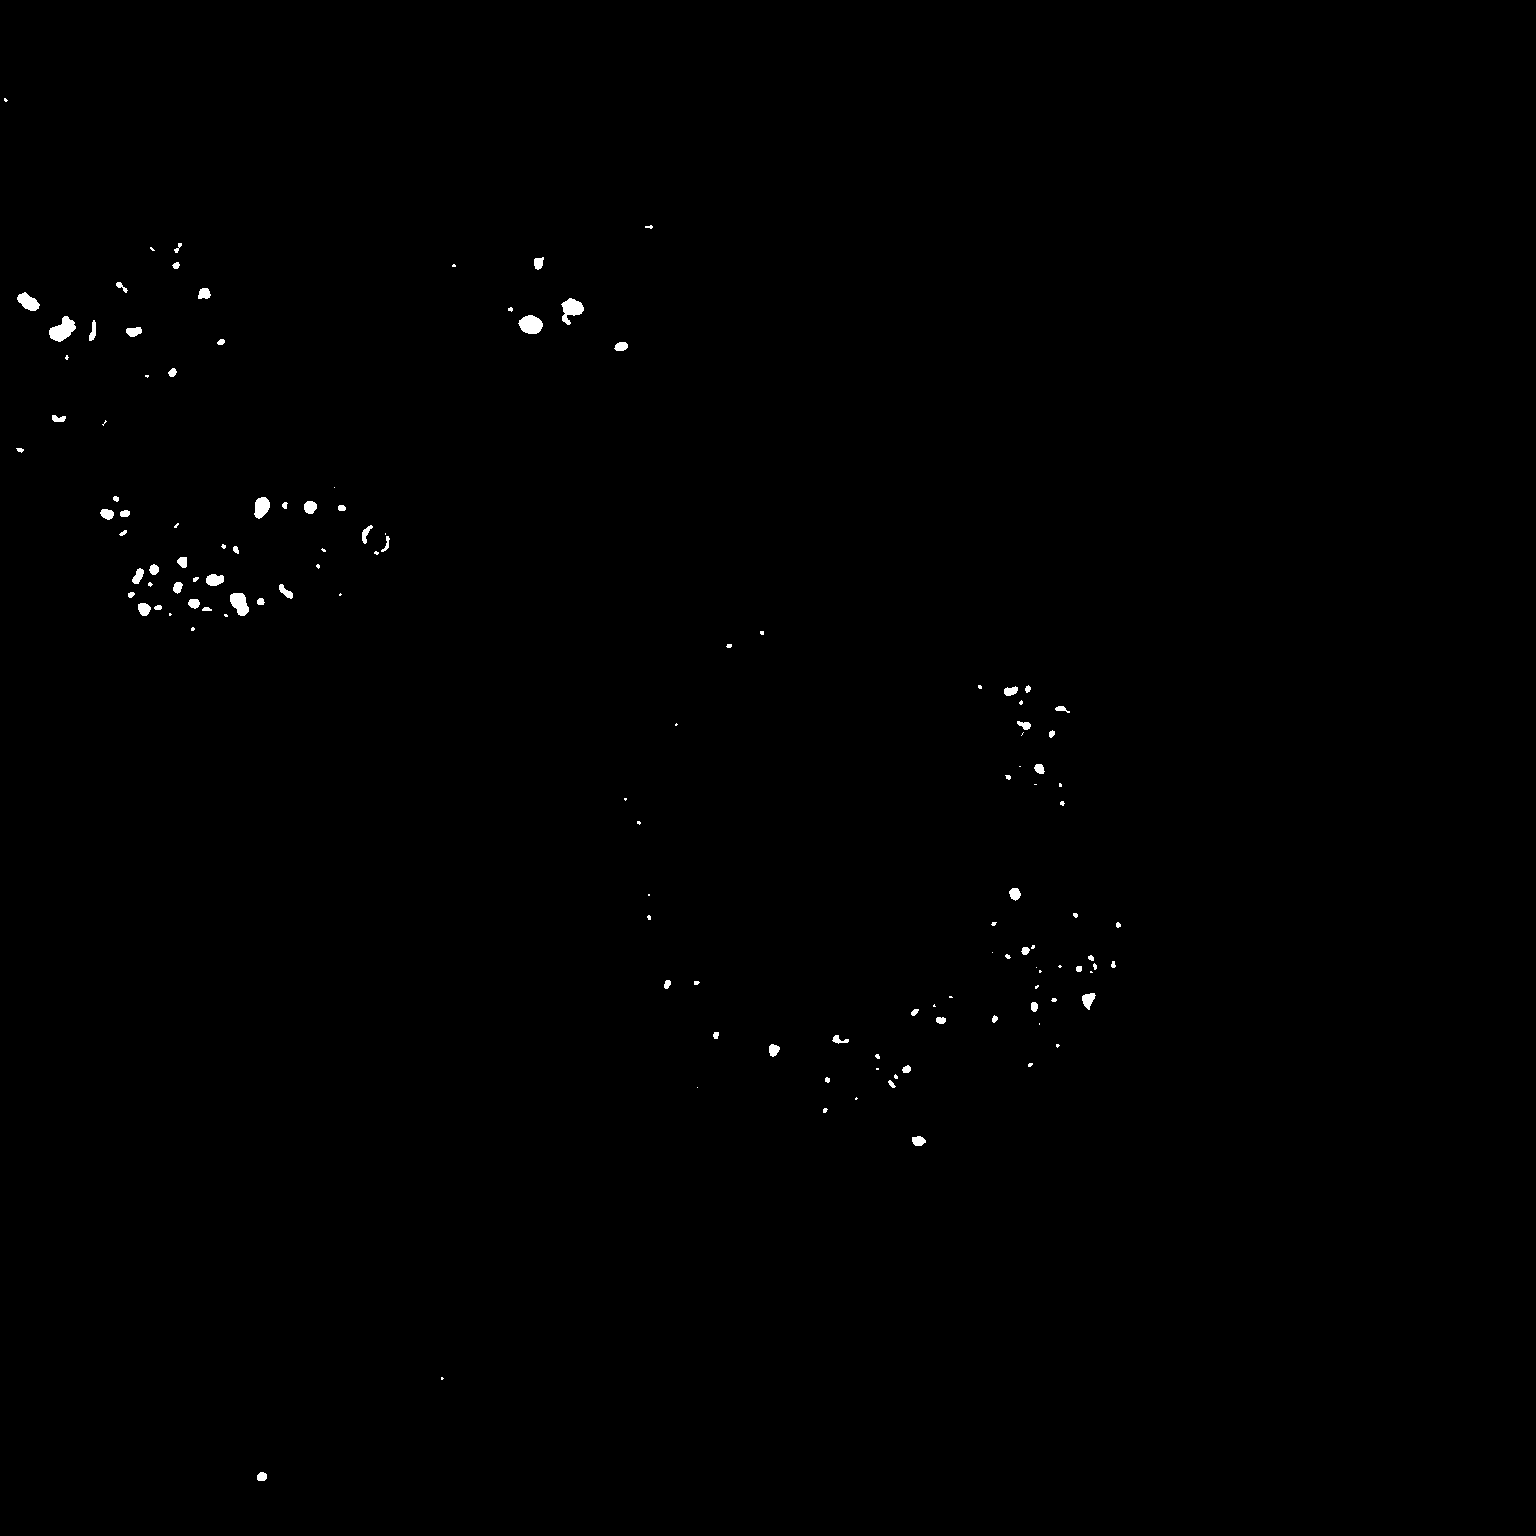
\includegraphics[width=0.24\textwidth]{figs/ch4figs/image_shortlisting/global/Shanbhag_LML_4C=1.png}}
	\subcaptionbox{MinError(I) applied to Sample 3}{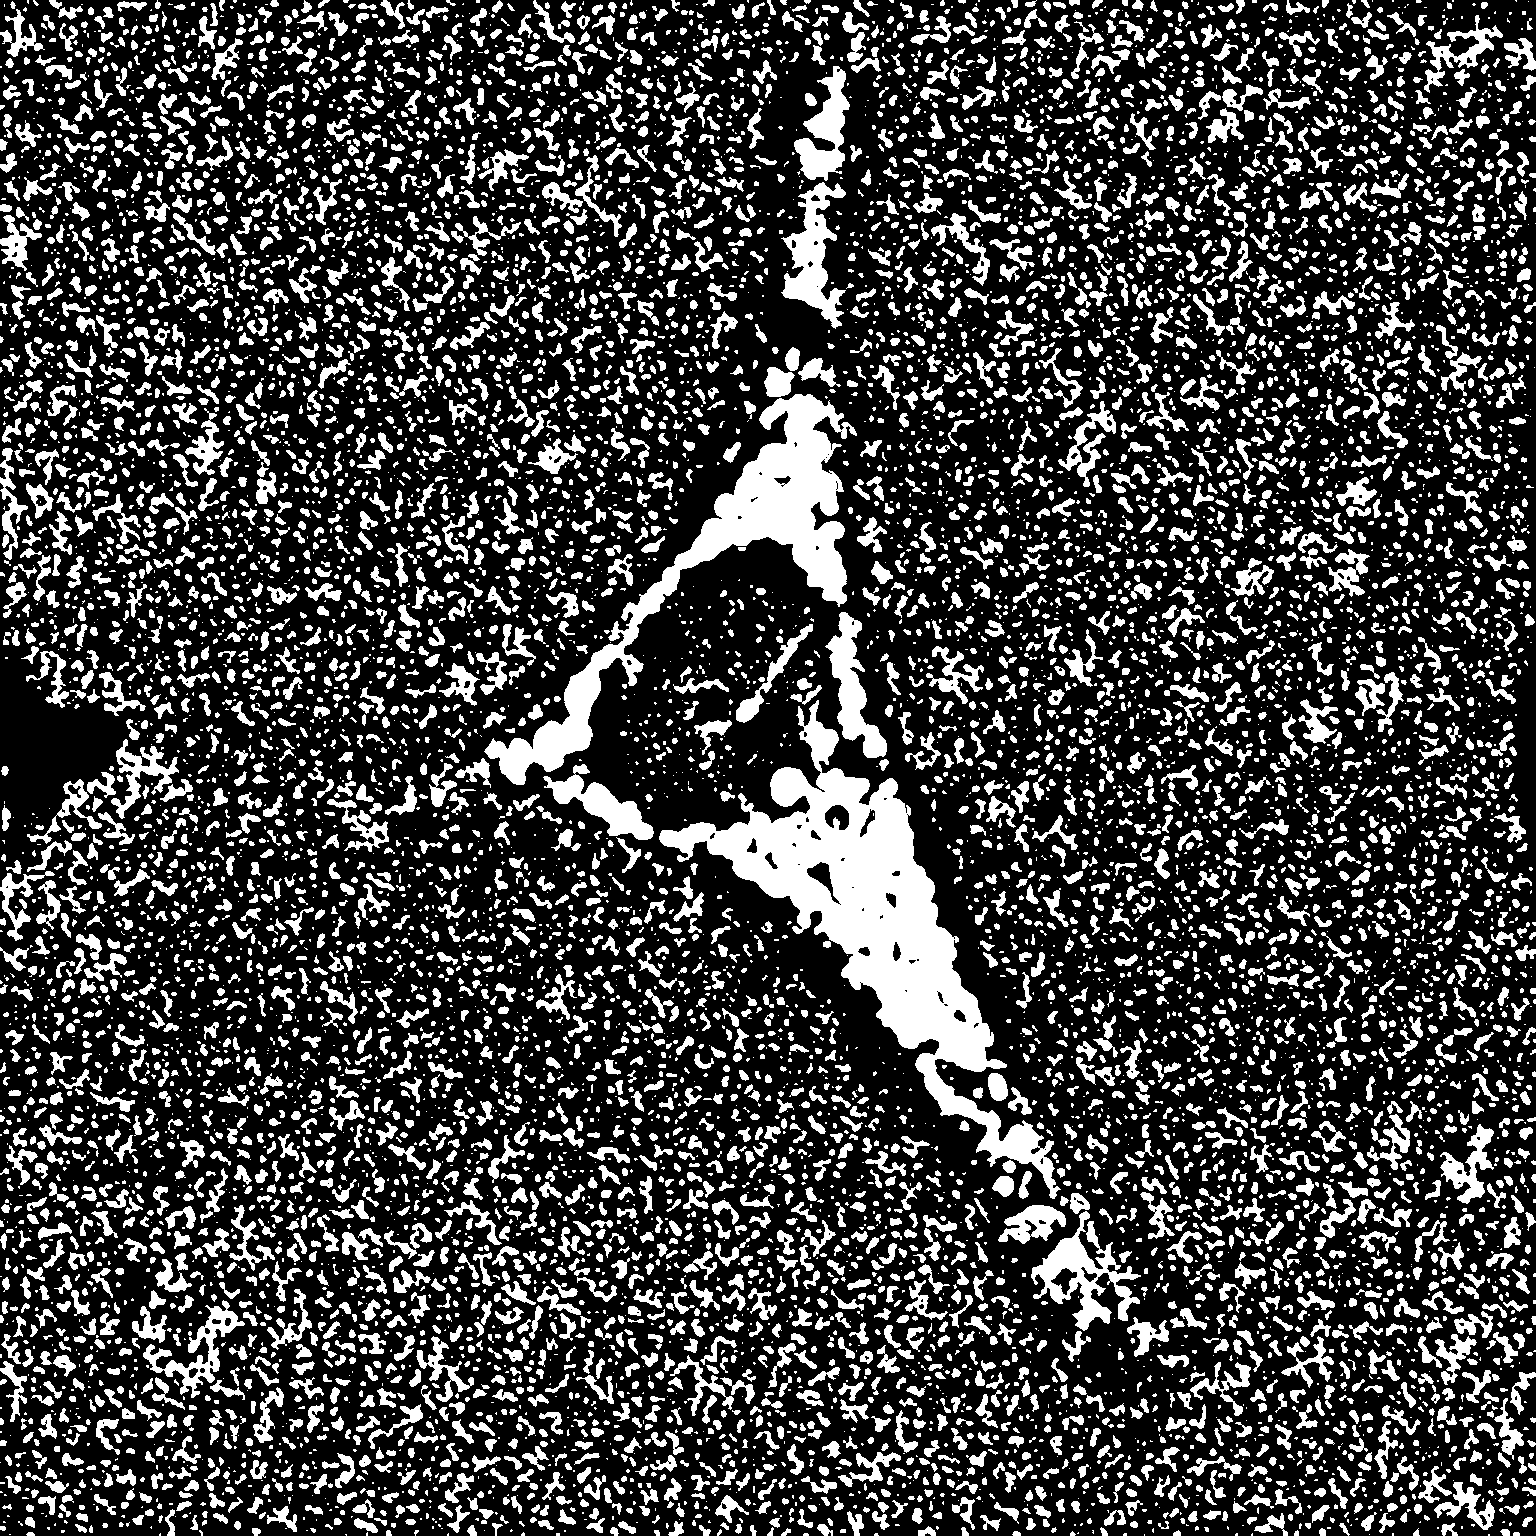
\includegraphics[width=0.24\textwidth]{figs/ch4figs/image_shortlisting/global/MinError(I)_LML_3C=0.png}}
	\subcaptionbox{Percentile applied to Sample 2}{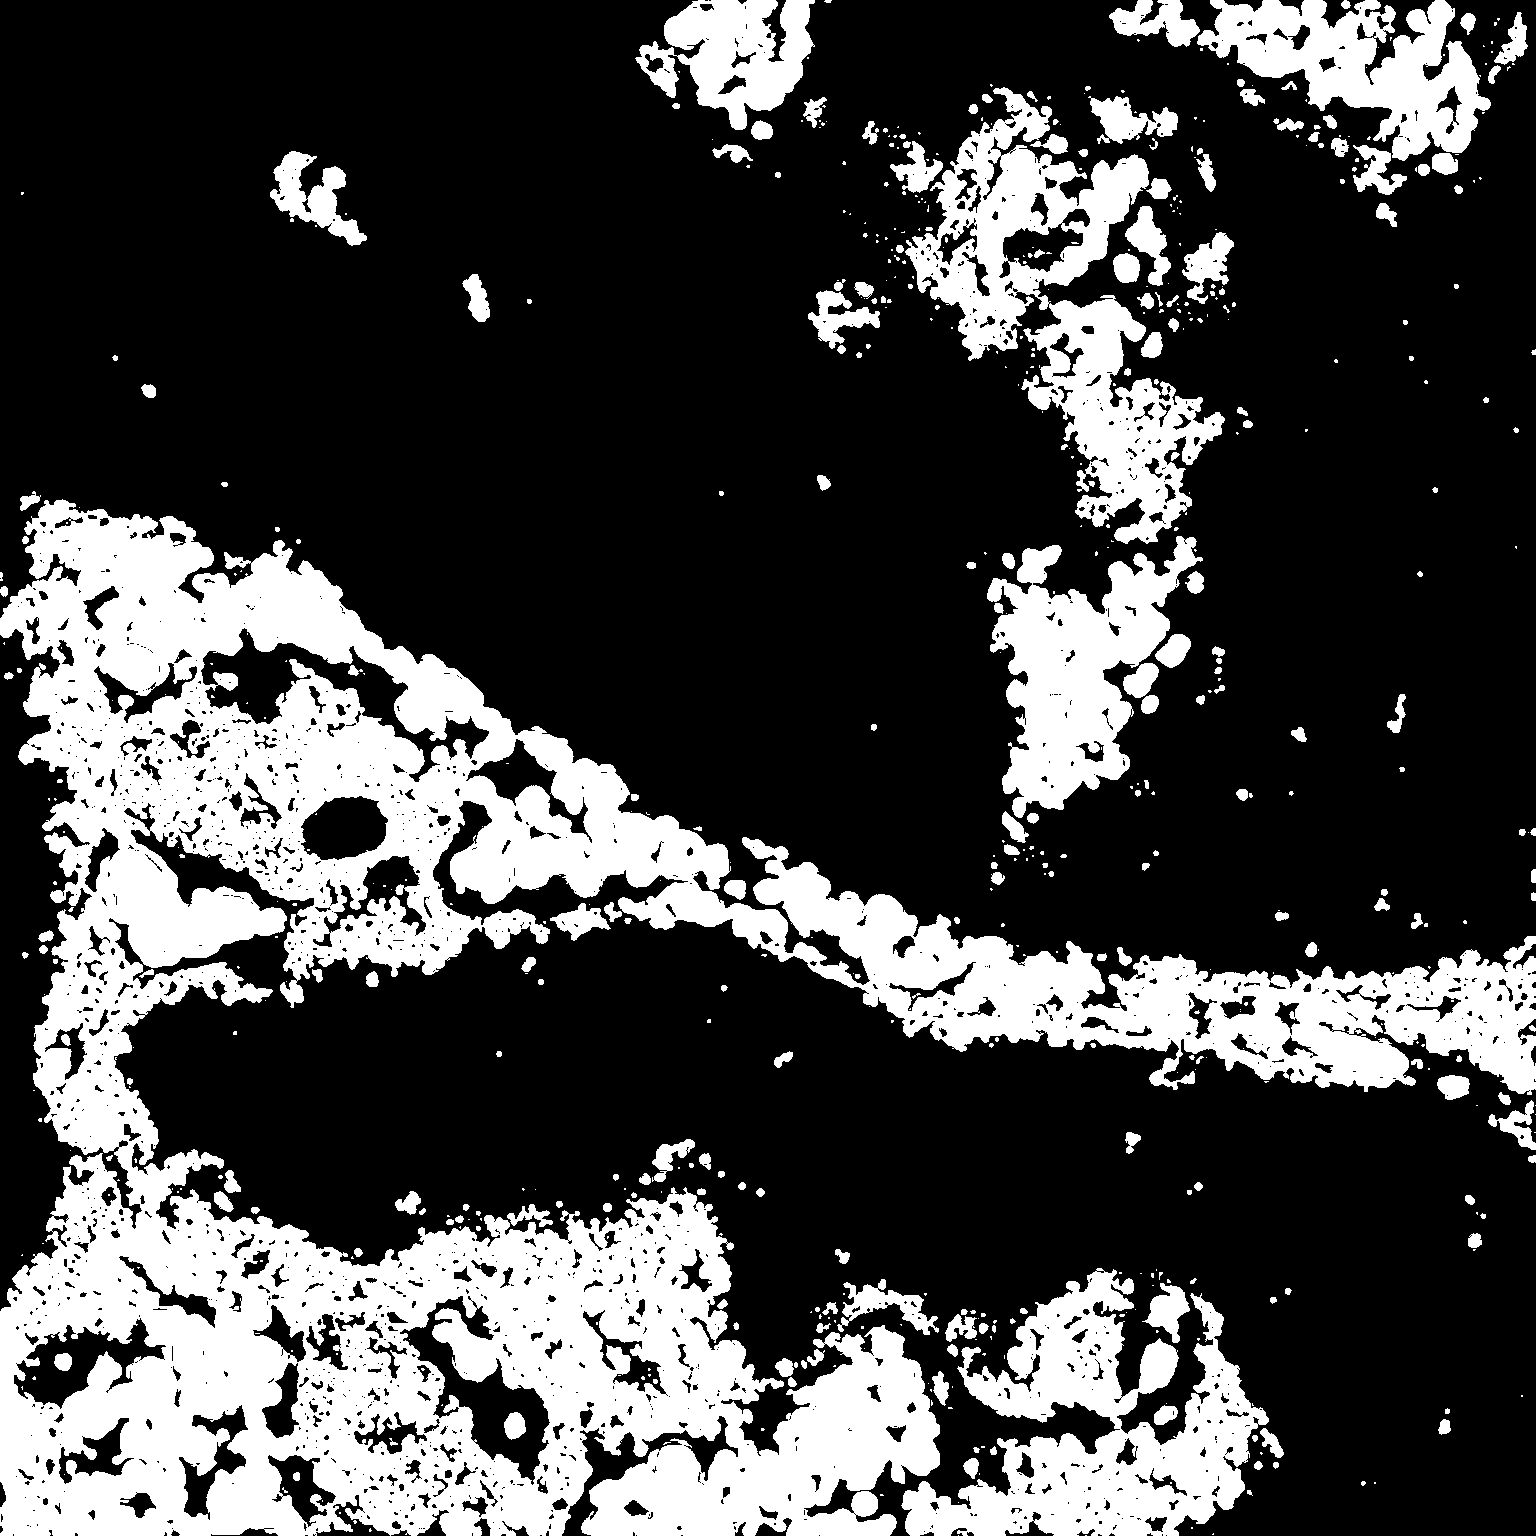
\includegraphics[width=0.24\textwidth]{figs/ch4figs/image_shortlisting/global/Percentile_HML_4C=0.png}}
	\subcaptionbox{Mean applied to \\Sample 1}{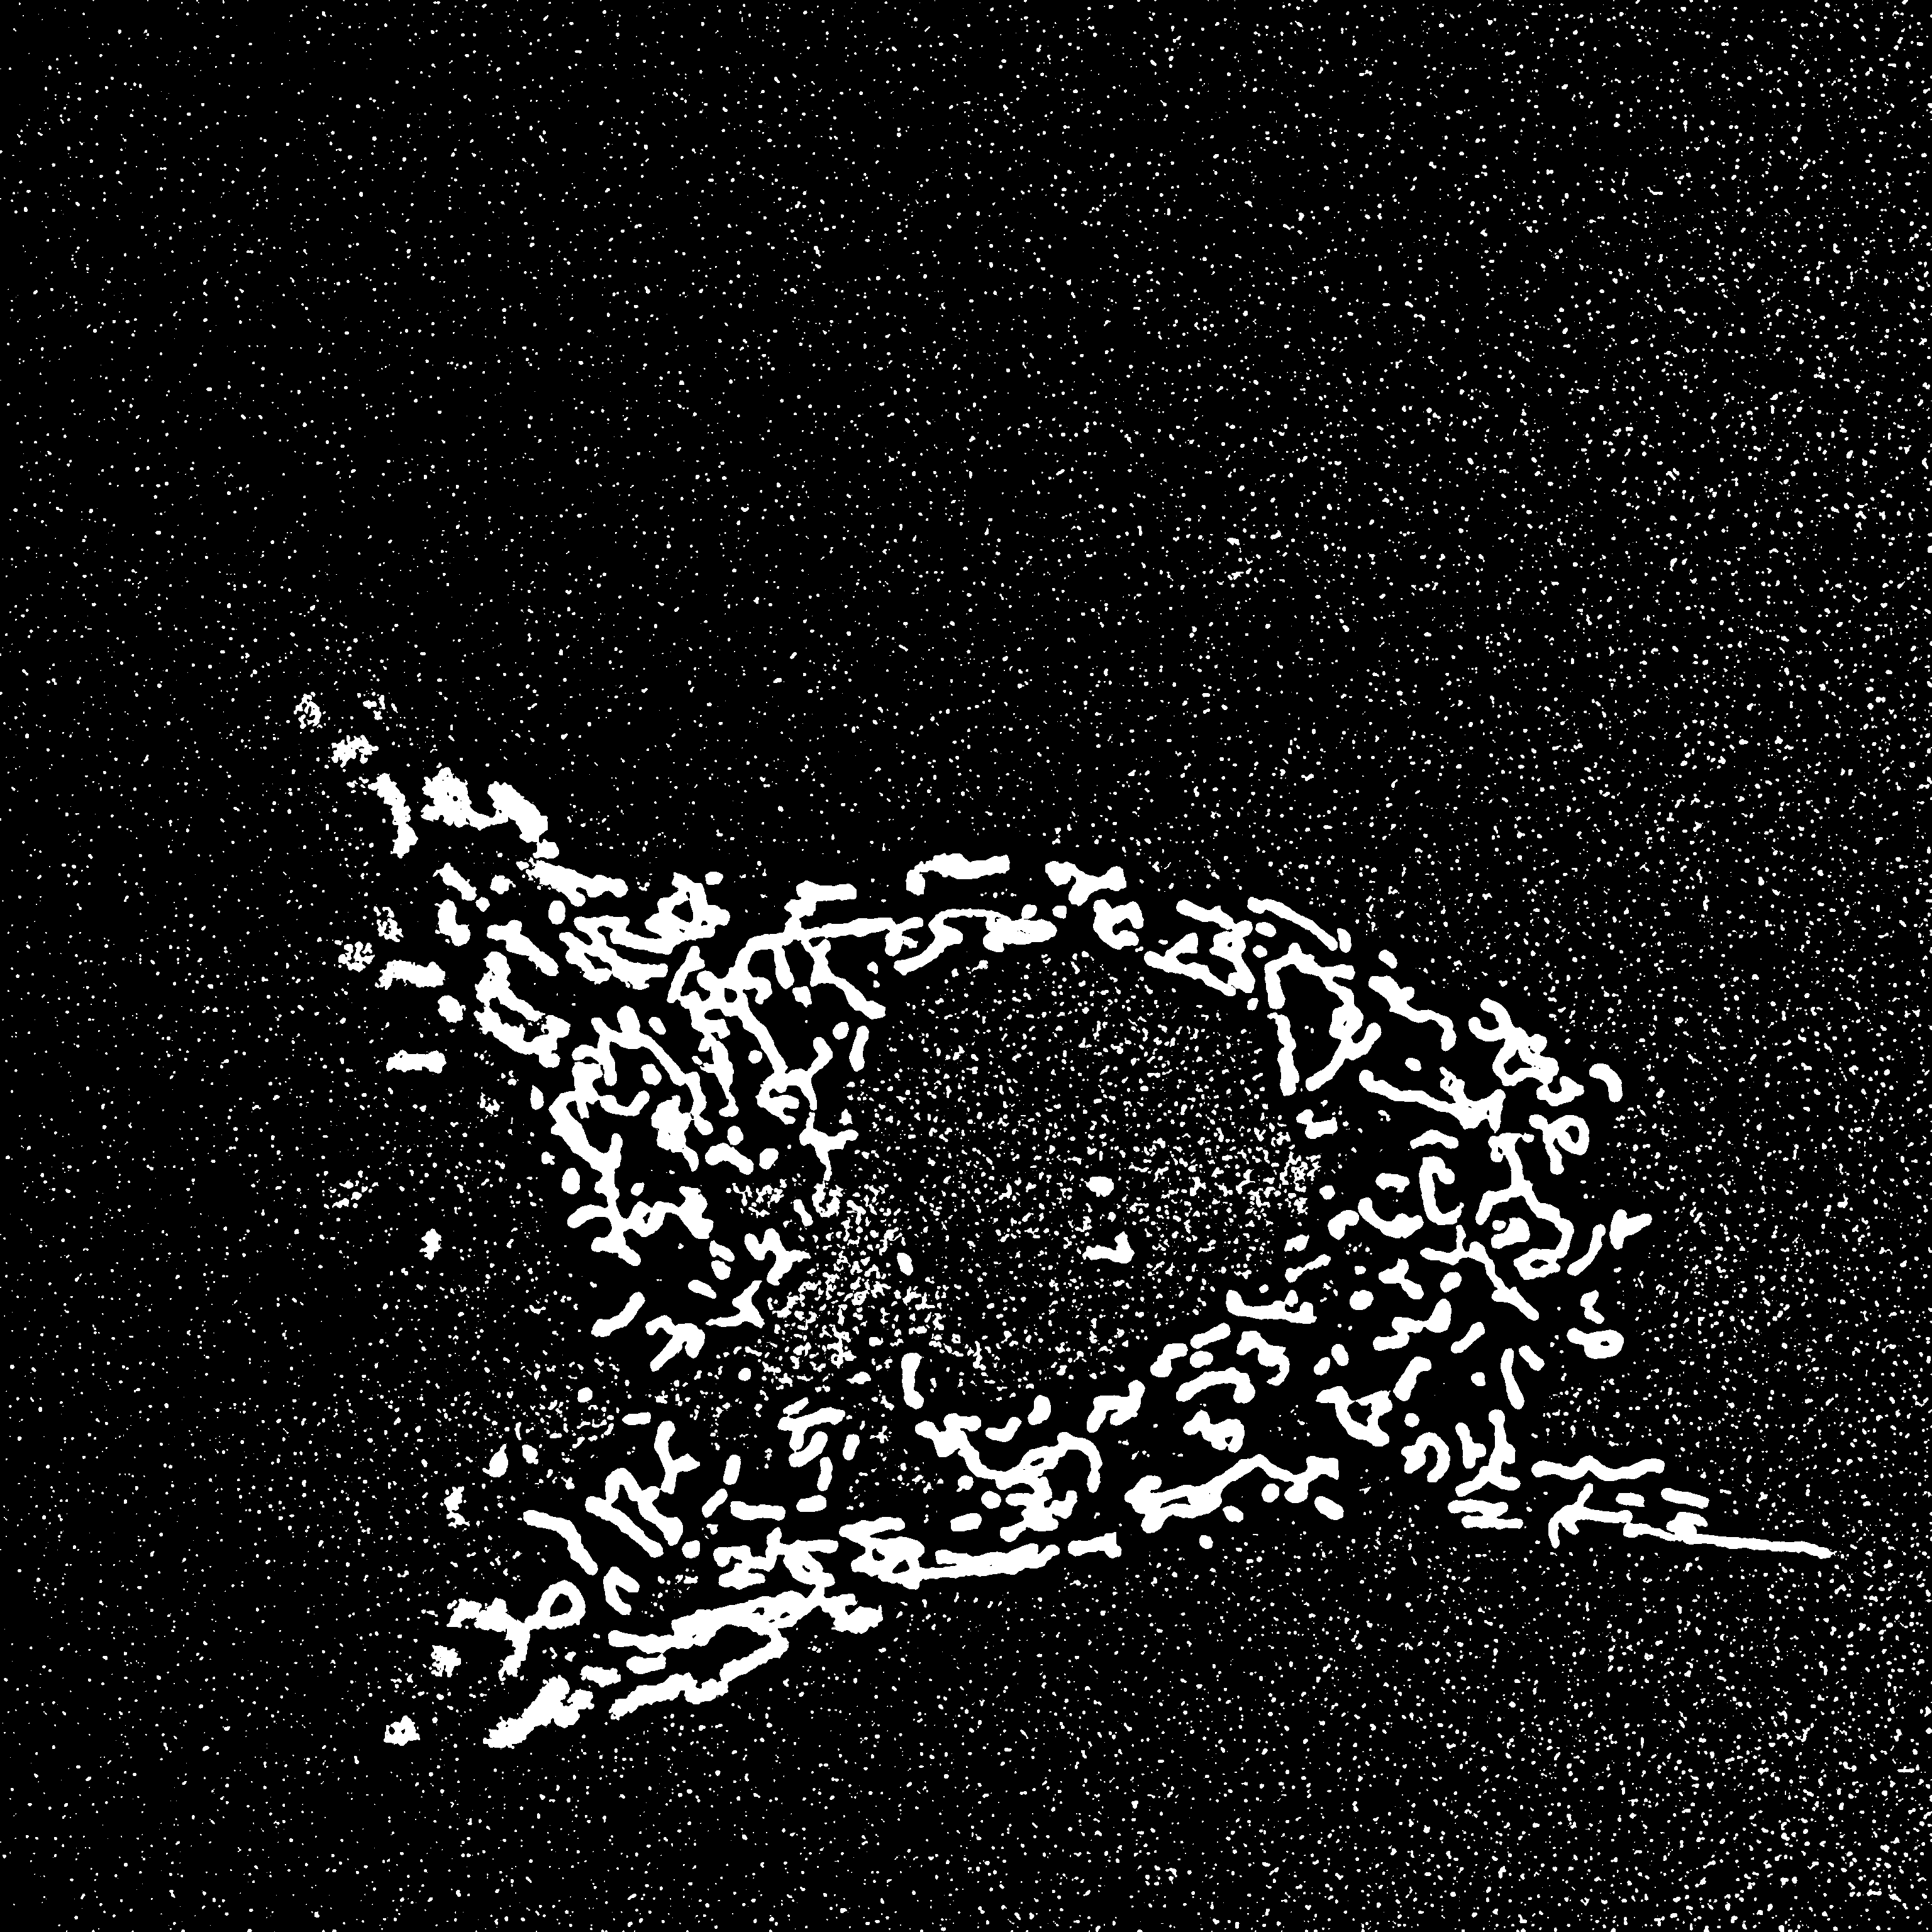
\includegraphics[width=0.24\textwidth]{figs/ch4figs/image_shortlisting/global/Mean_CCCP_1C=1T=0.png}}
	\subcaptionbox{Huang applied to Sample 4}{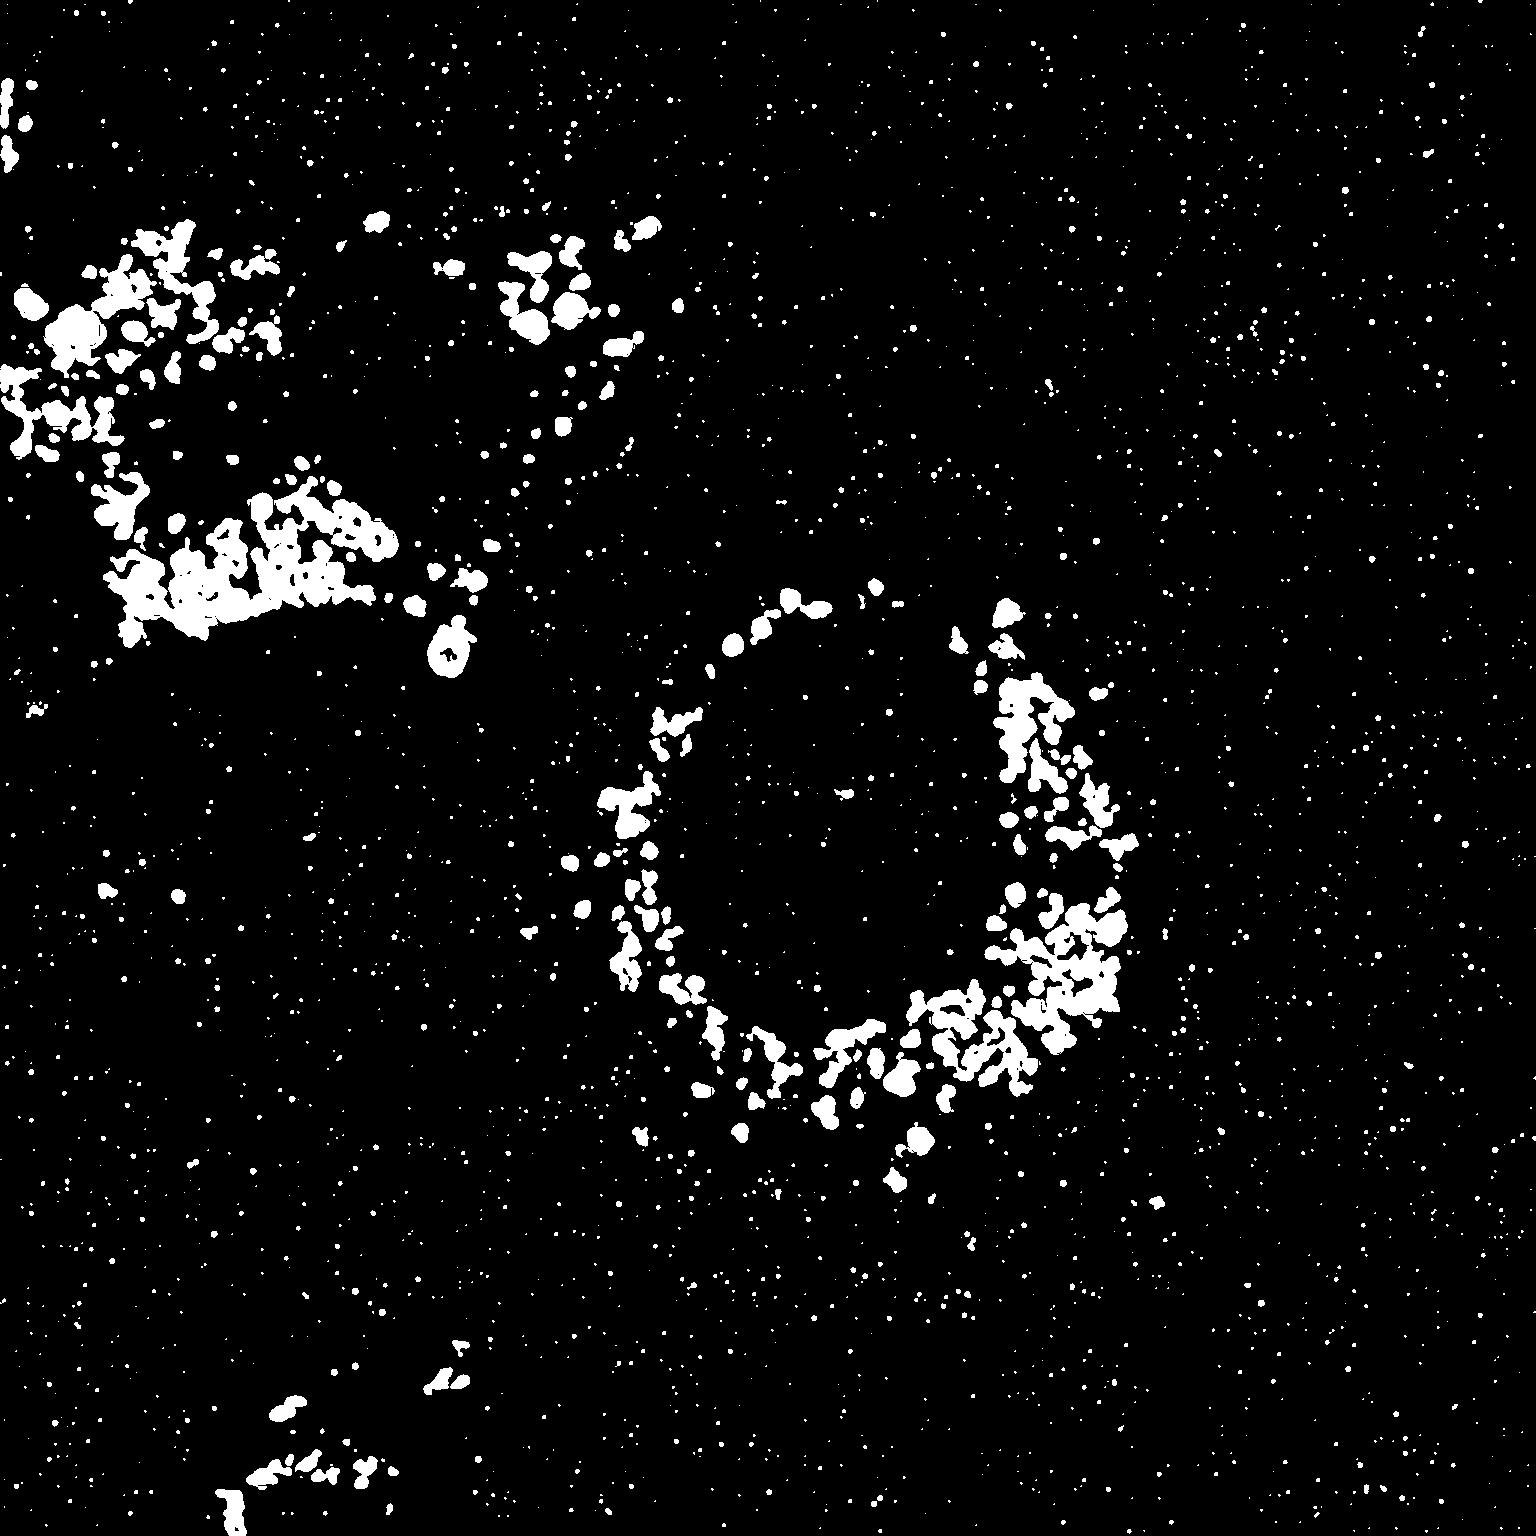
\includegraphics[width=0.24\textwidth]{figs/ch4figs/image_shortlisting/global/Huang_LML_4C=1.png}}
	\caption[Showcase of non-viable global threshold outcomes for the shortlisting data set.]{Showcase of non-viable global threshold outcomes for the shortlisting data set. The samples showcased are chosen to represent the shortcoming of these methods for the real sample images shown in Figure \ref{fig:shortlist_raw}.}
	\label{fig:bad_global_subset}
\end{figure}
\FloatBarrier
\subsection{Local threshold shortlisting}
A total of 9 local thresholding methods, provided by the ``Auto Local Threshold'' plug-in, were evaluated for viable application to the sample images. These methods are:
\begin{multicols}{3}
	\begin{itemize}
		\setlength\itemsep{1mm}
		\item Bernsen
		\item Contrast
		\item Mean
		\item Median
		\item MidGrey
		\item Niblack
		\item Otsu
		\item Phansalkar
		\item Sauvola
	\end{itemize}
\end{multicols}
Compared to global thresholding methods, the shortlisting of local thresholding methods is a bit more involved due to the tuning of parameters being required for fair evaluation of these methods. All local thresholding methods binarize each pixel based on a pixel-specific threshold where this threshold is determined using a localized region, or window, surrounding said pixel. The size of this neighbourhood can greatly influence the binarization outcome thus selection of an appropriate window size for each image is crucial for every method. Additionally, all local thresholding methods being assessed, save for Contrast and Otsu, provide additional parameters that can be tuned to further influence the binarization. For rapid application of these local thresholds it is not uncommon to approximate parameters that best generalize across the sample set based on the binarization performance for a smaller subset. For this reason, the shortlisting will evaluate the local thresholding methods with performance considered with respect to the parameter selections, per method, that generalize best across all of the shortlisting samples. 
\paragraph{Findings:} From observations of the local thresholding outcomes, the methods deemed viable for further use in evaluations were Bernsen, Mean, Median, and MidGrey. Furthermore, the optimal window size was selected as 15 as Bernsen and MidGrey both exhibit a growing risk of over-thresholding at higher window sizes, as seen in Figure \ref{fig:local_window_size_showcase}, while Mean and Median still provide sufficient threshold outcomes. The effects of parameter tuning for these methods are shown in Figure \ref{fig:local_param_tuning} with RGB images with the different colour channels representing the thresholding outcome under different secondary parameters while a second row depicts the parameter selection deemed ``optimal'' with better clarity than the RGB images. For Bernsen, the colour channels represent the contrast threshold parameter values which are $10$ for Red, $15$ for Green, and $20$ for Blue. The default value provided by Fiji was $15$ thus the variations in the parameter value were centred around this. It was observed that the Red channel captured too much noise in the image (minor under-thresholding) while the Blue channel (only seen as white due to channel overlap) captured a few fewer structures than the Green and Red channels respectively the Green channel ($15$) was deemed as the optimal middle ground. For the Mean, Median, and MidGrey threshold methods, the colour channels represent the subtract constant parameter values which are $0$ for Red, $-5$ for Green, and $5$ for Blue. The colour channel to parameter mappings was selected to visualise with the best clarity as the Blue channel depicts gross under-thresholding, with the background almost completely blue, which the Red channel overlaps with as magenta. It was observed that for all of these methods both the Red and Blue channels depict under-thresholding of minor and major severities respectively while the Green channel ($-5$) provides the best outcome generalized across the shortlisting samples. \par The outcomes for all shortlisting samples at the varied window size parameter and secondary parameter tunings can be viewed in Appendix \ref{appen_sec:local_shortlist} for all methods (both those deemed viable and non-viable).

\begin{figure}
	\centering
	\subcaptionbox{Median with a \\Window size of 15}{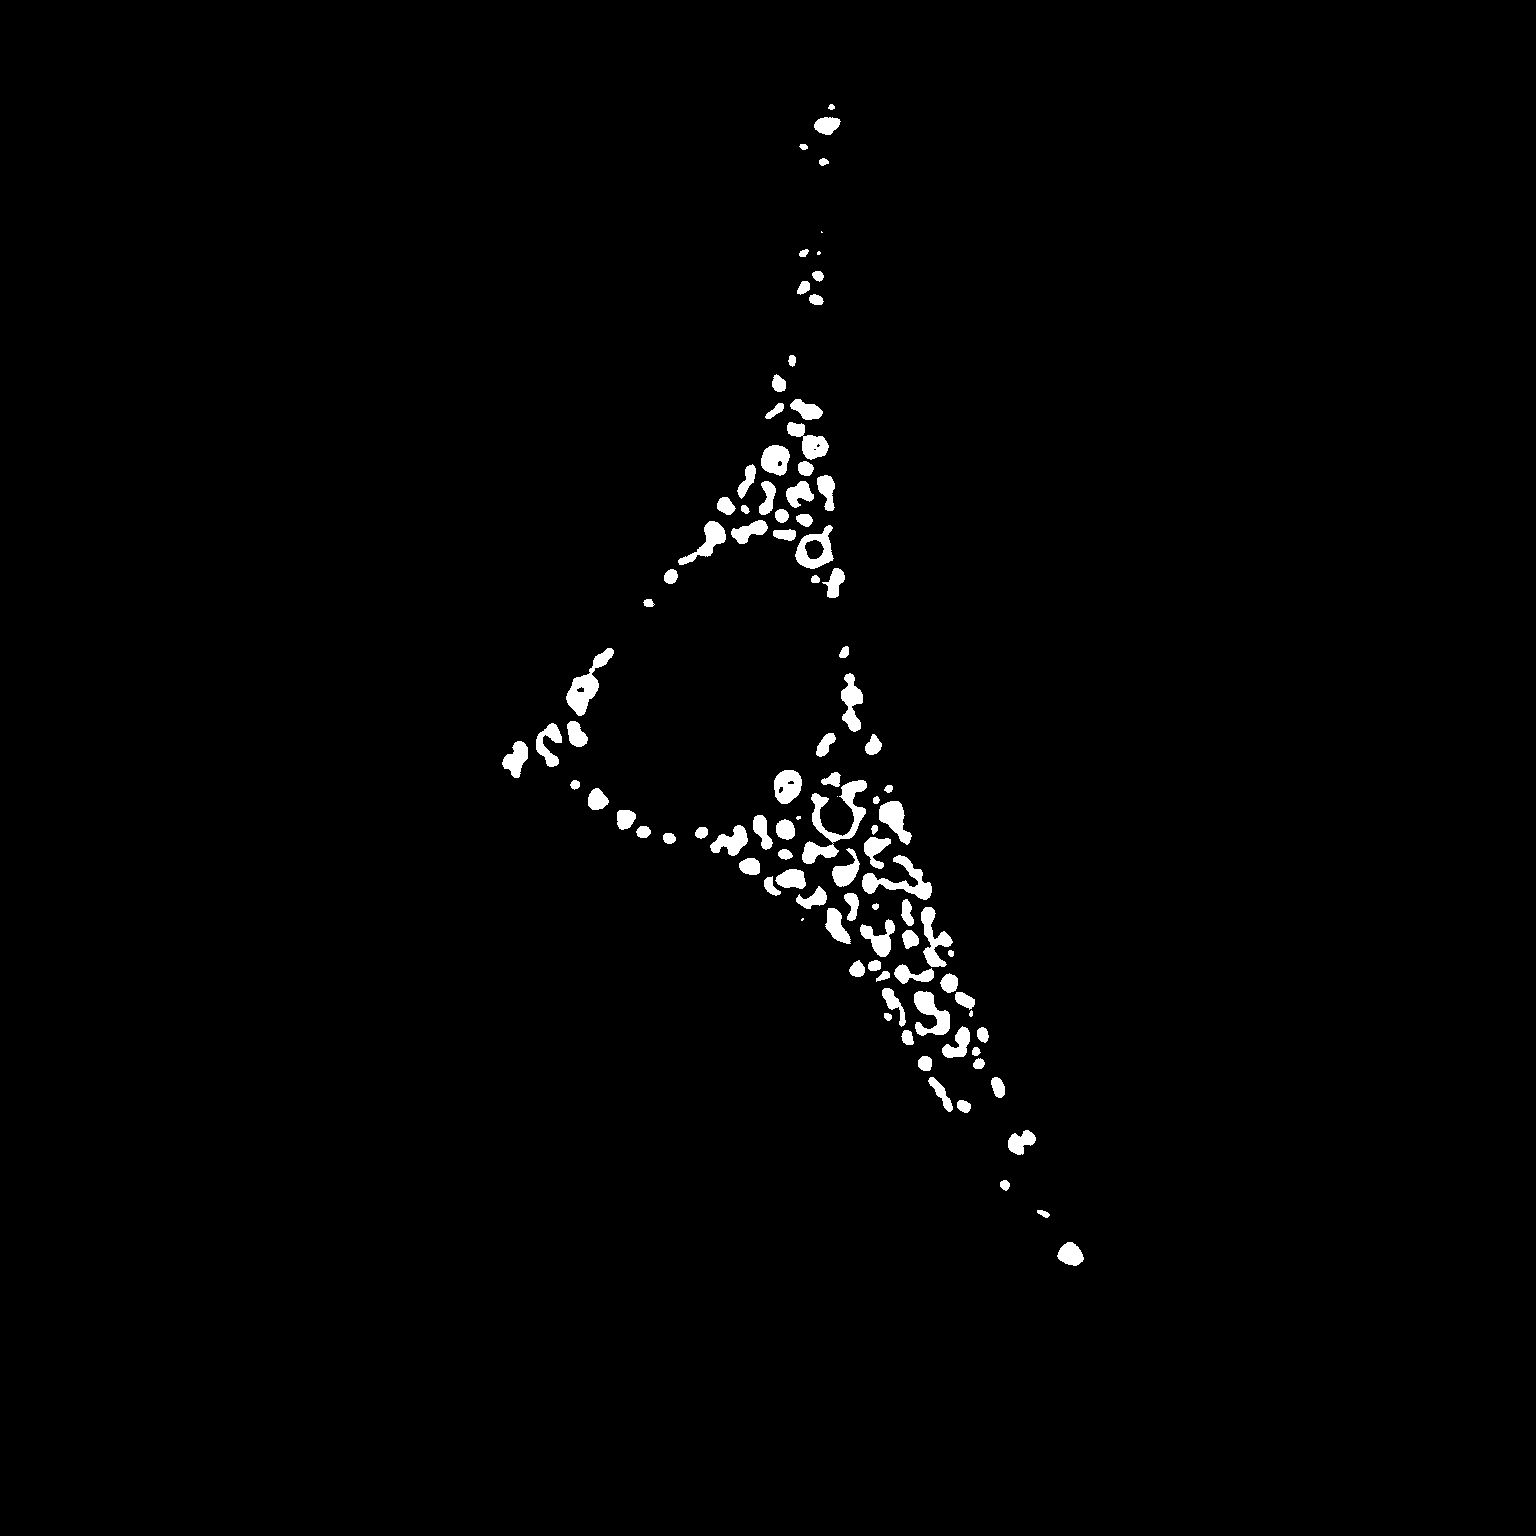
\includegraphics[width=0.3\textwidth]{figs/ch4figs/image_shortlisting/local/Median_p-5_w15_LML_3C=0.png}}
	\subcaptionbox{Median with a \\Window size of 60}{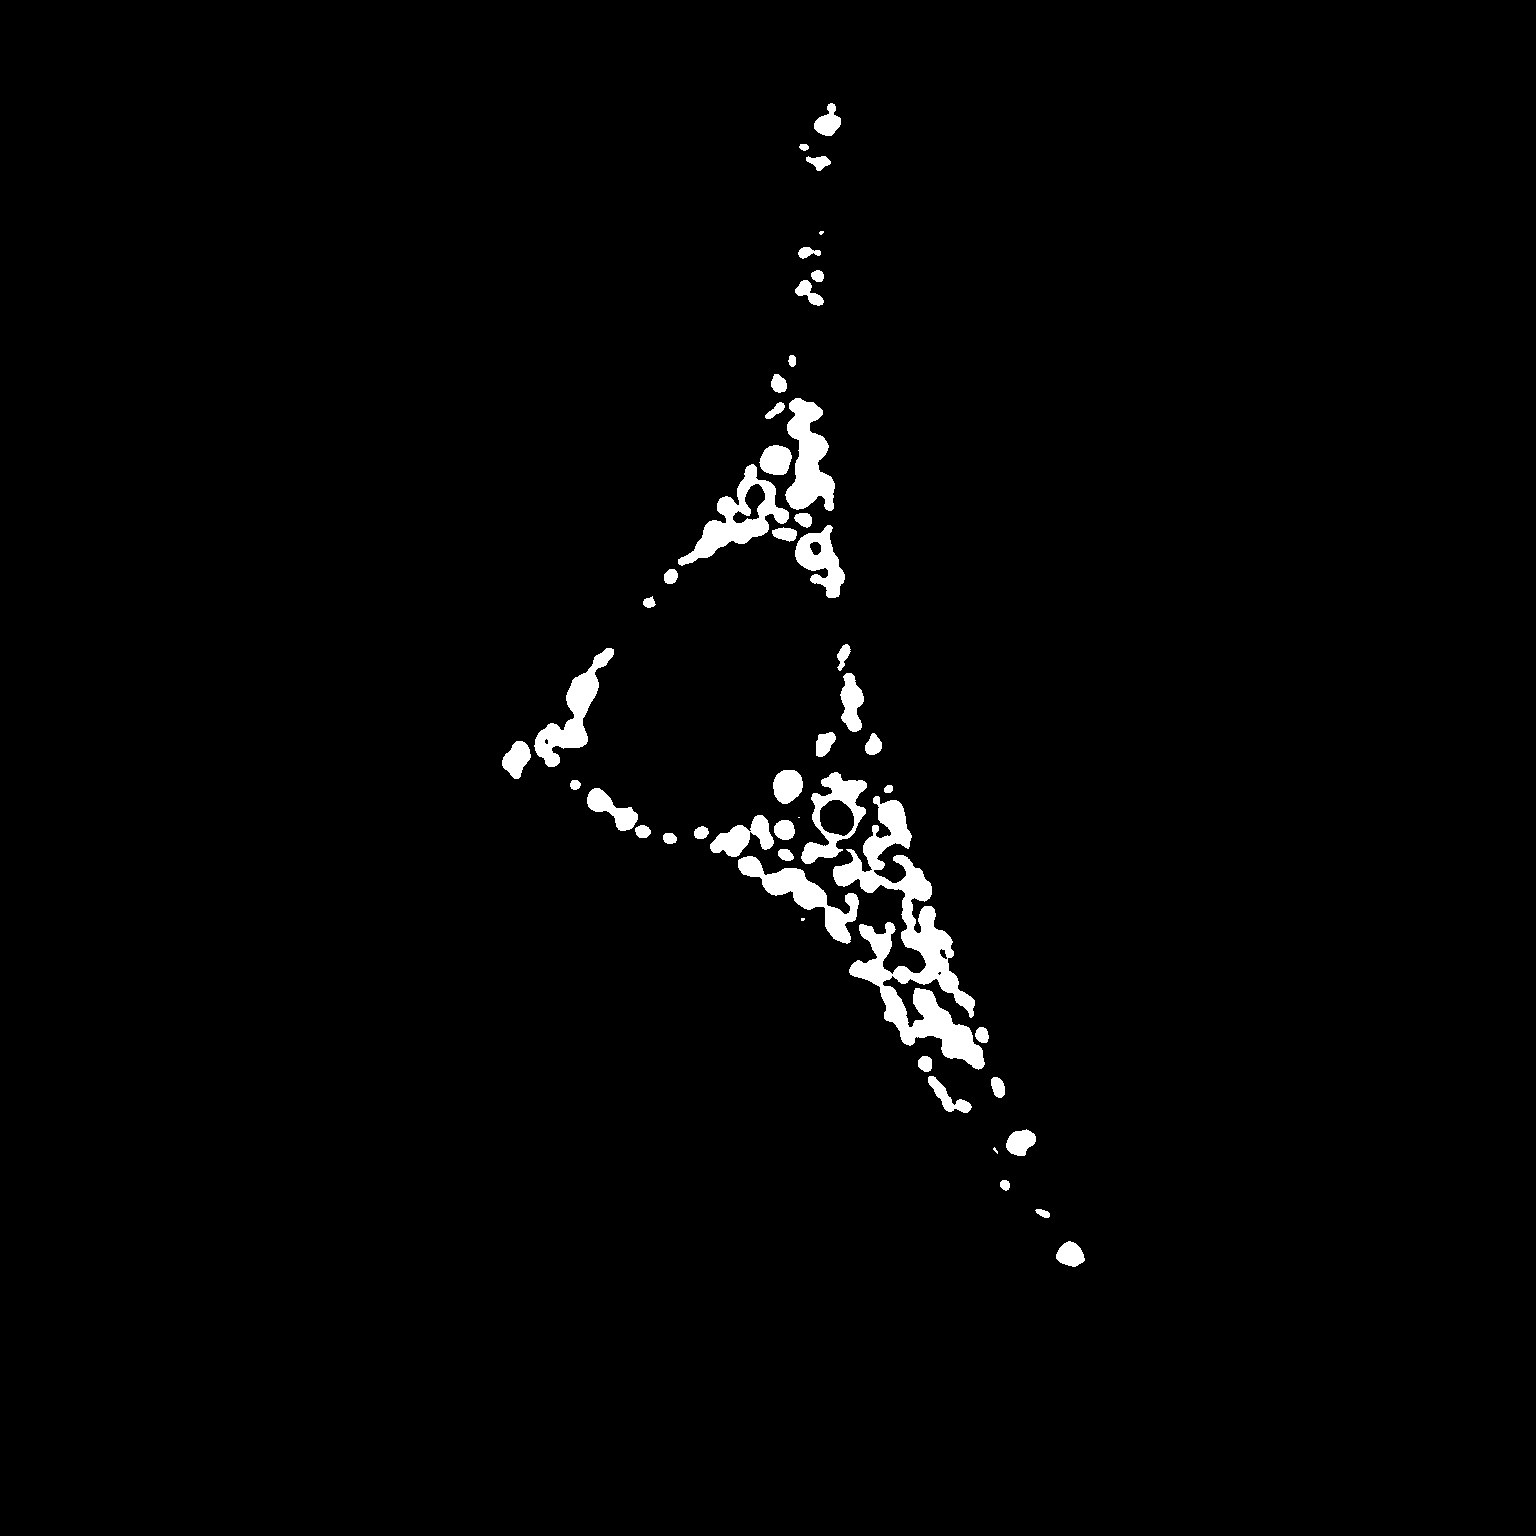
\includegraphics[width=0.3\textwidth]{figs/ch4figs/image_shortlisting/local/Median_p-5_w60_LML_3C=0.png}}
	\subcaptionbox{Median with a \\Window size of 100}{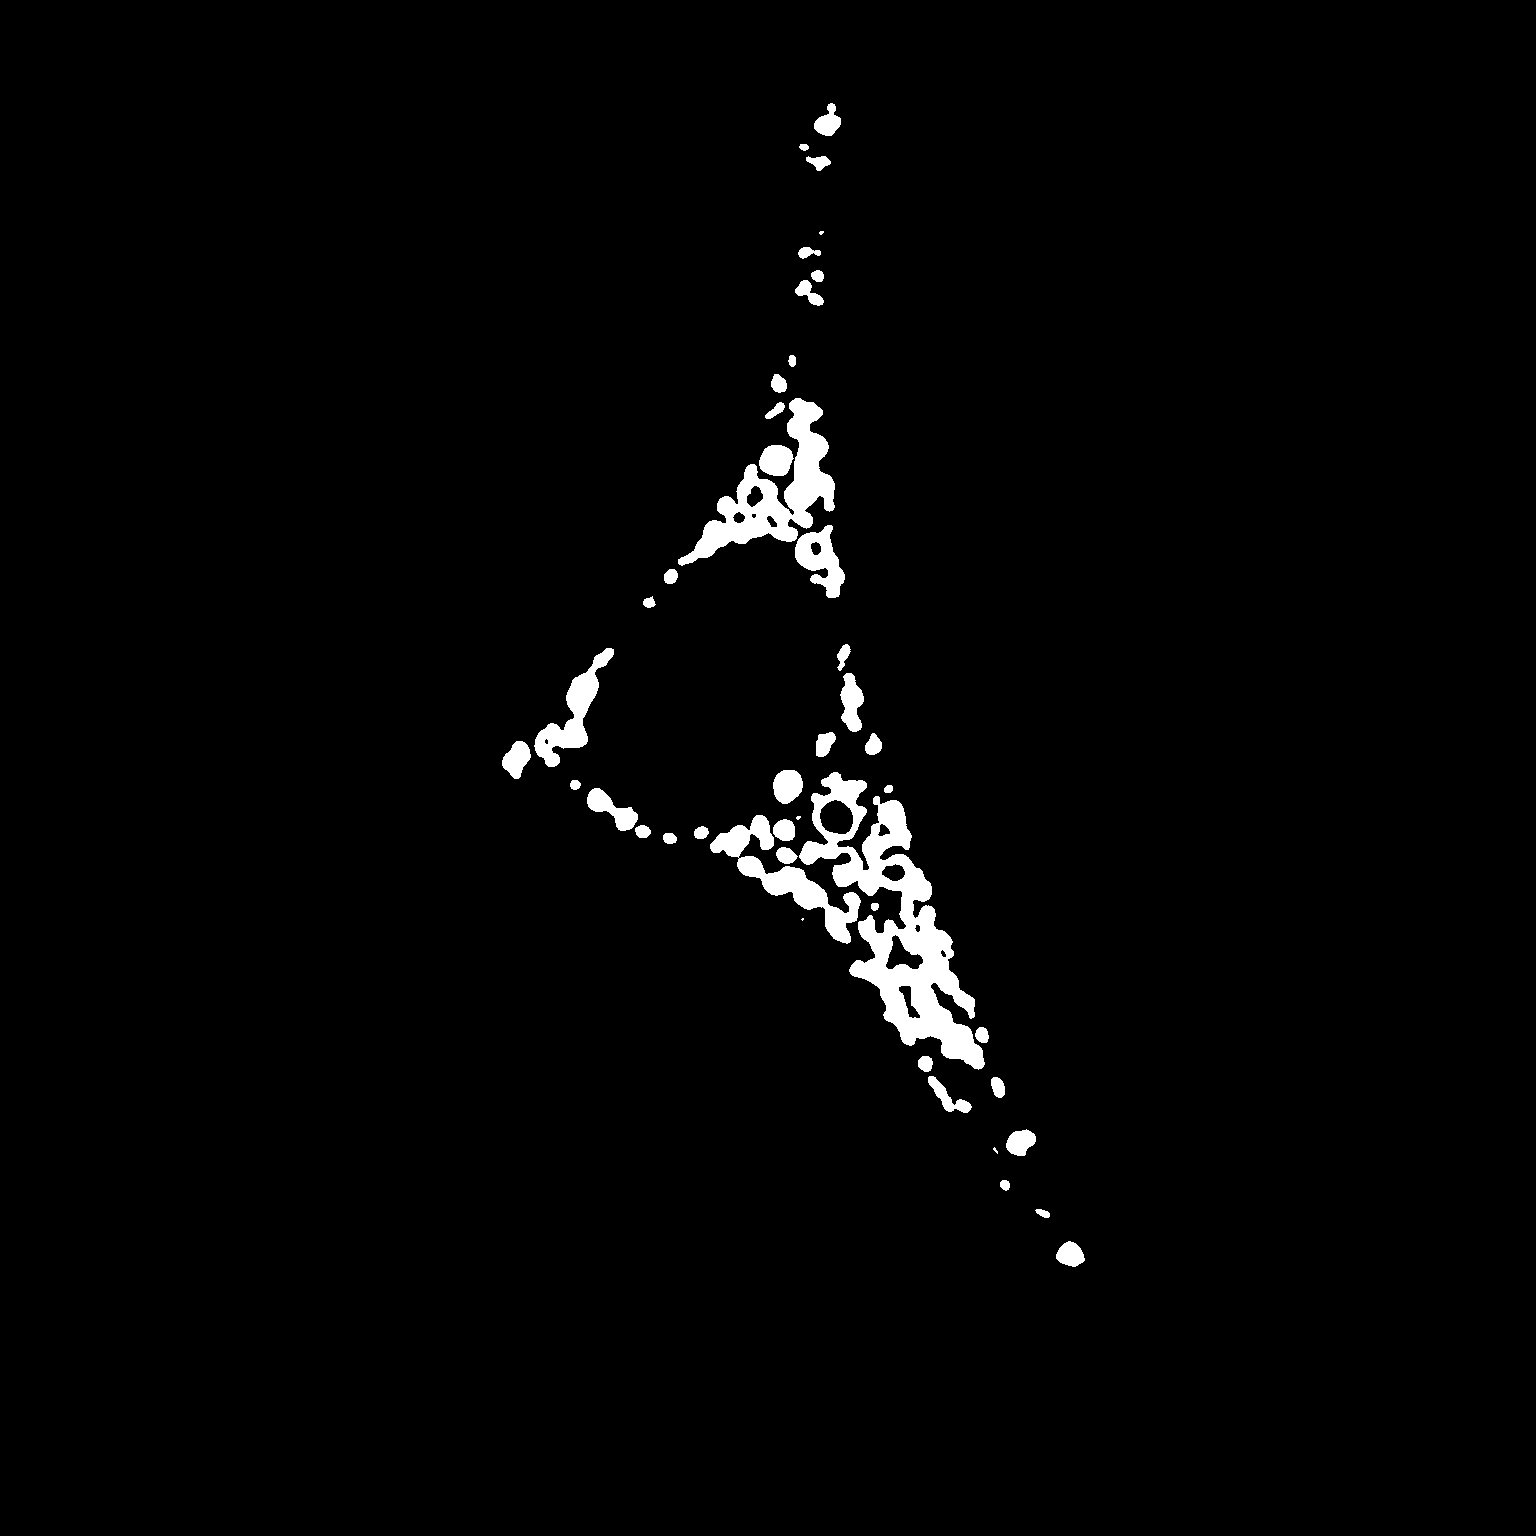
\includegraphics[width=0.3\textwidth]{figs/ch4figs/image_shortlisting/local/Median_p-5_w100_LML_3C=0.png}}
	\subcaptionbox{MidGrey with a \\Window size of 15}{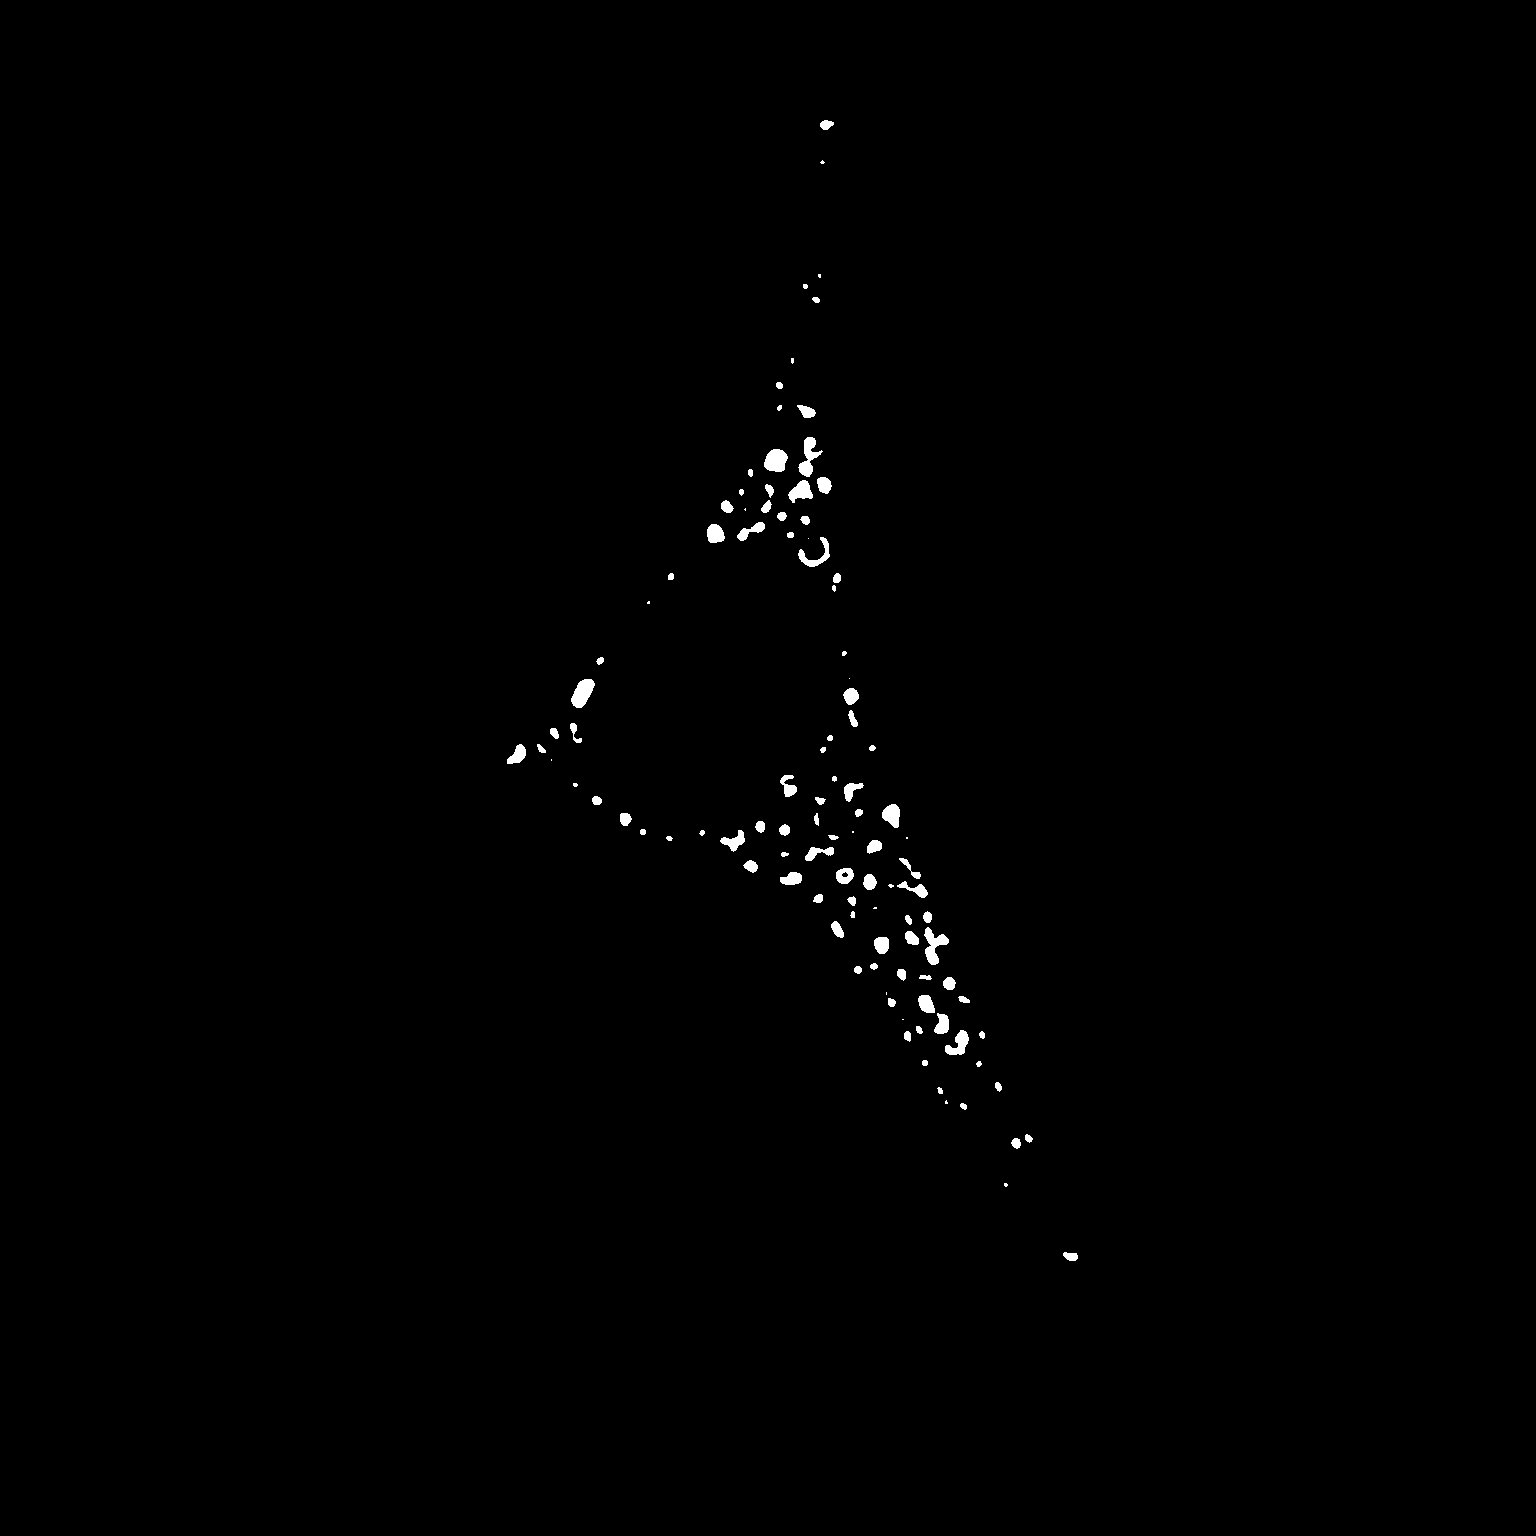
\includegraphics[width=0.3\textwidth]{figs/ch4figs/image_shortlisting/local/MidGrey_p-5_w15_LML_3C=0.png}}
	\subcaptionbox{MidGrey with a \\Window size of 60}{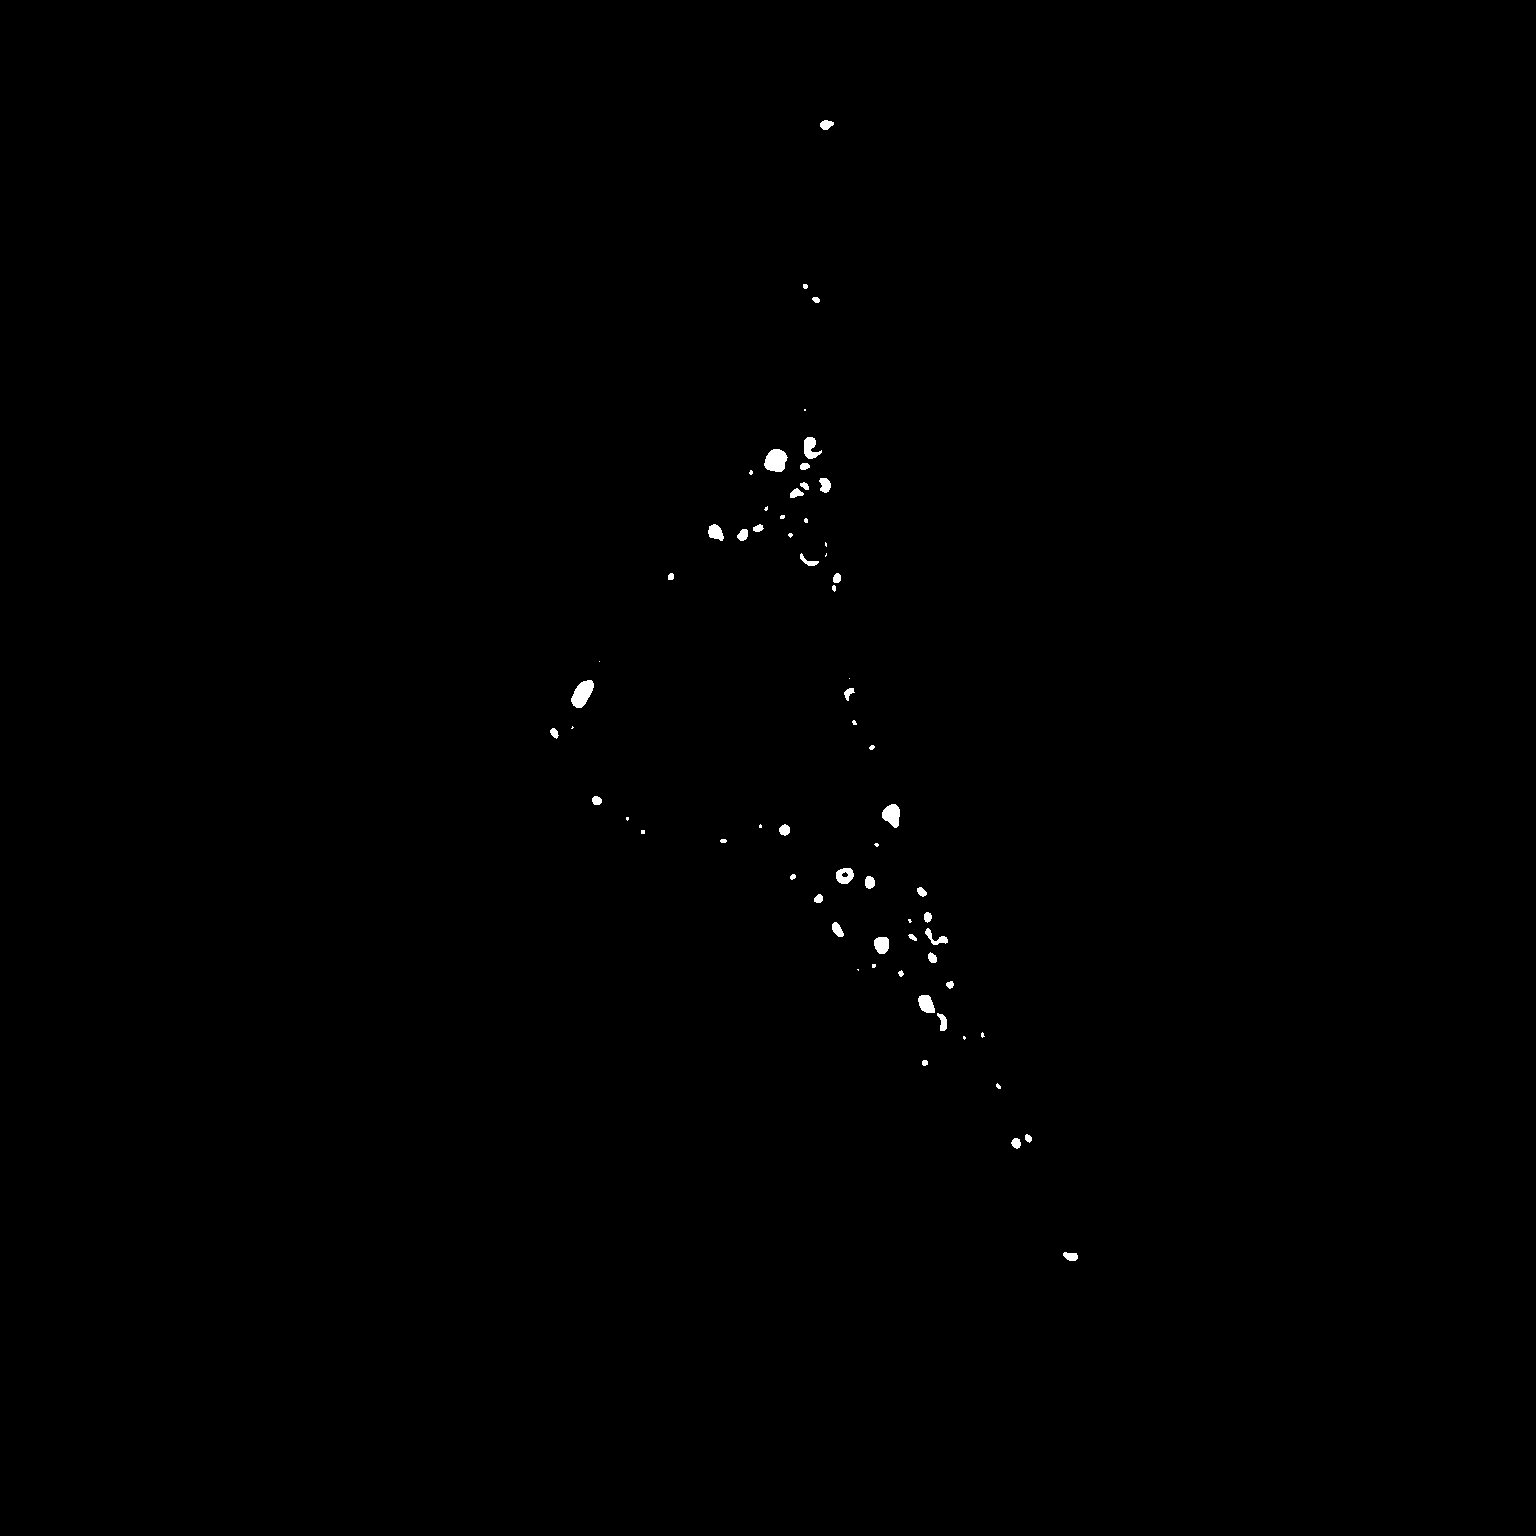
\includegraphics[width=0.3\textwidth]{figs/ch4figs/image_shortlisting/local/MidGrey_p-5_w60_LML_3C=0.png}}
	\subcaptionbox{MidGrey with a \\Window size of 100}{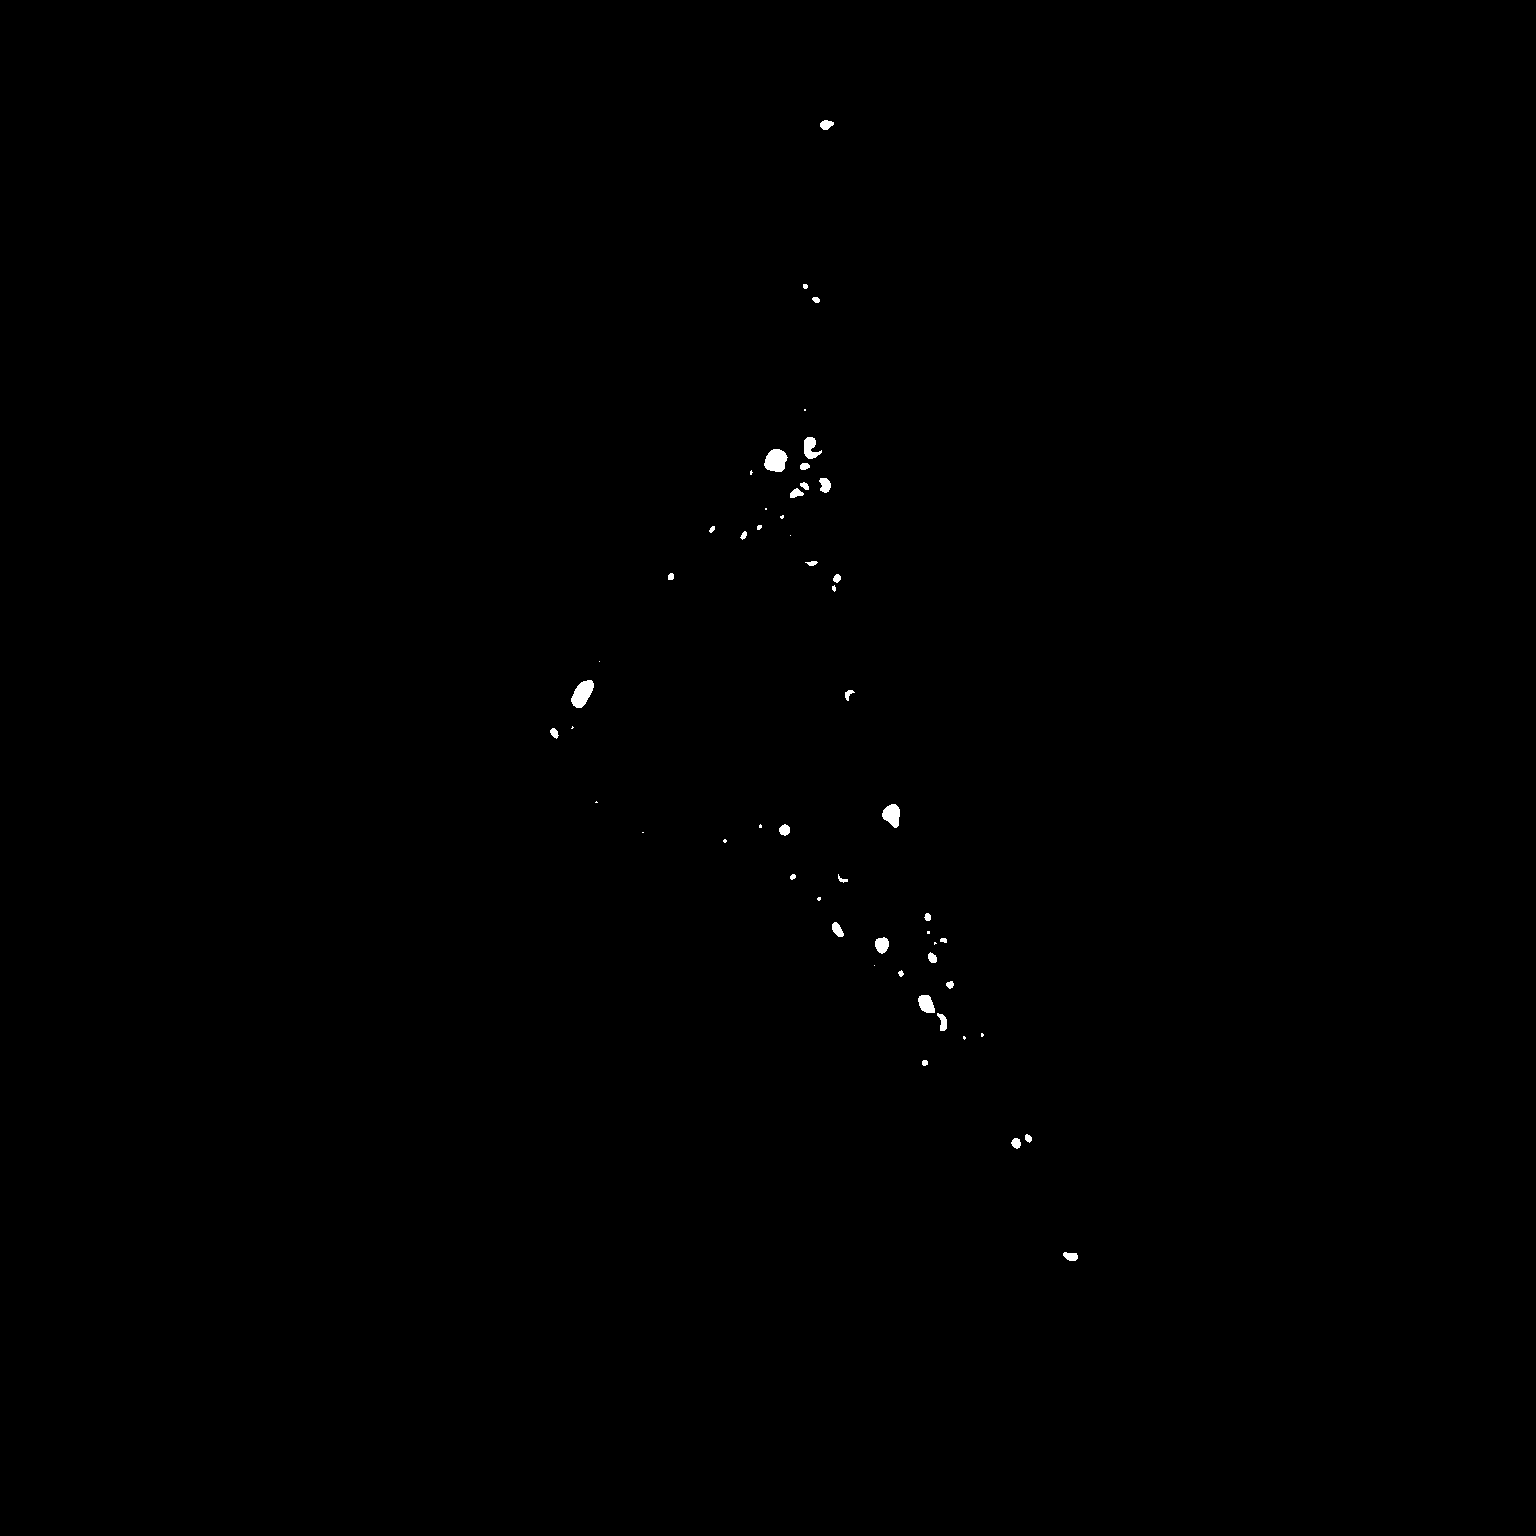
\includegraphics[width=0.3\textwidth]{figs/ch4figs/image_shortlisting/local/MidGrey_p-5_w100_LML_3C=0.png}}
	\caption[Showcasing the impact larger window sizes can have on local thresholding outcomes.]{Showcasing the impact larger window sizes can have on local thresholding outcomes. For this example the Median and MidGrey thresholding methods have been applied to sample 3 with a subtraction constant of $-5$.}
	\label{fig:local_window_size_showcase}
\end{figure}
 
\begin{figure}
	\centering
	\subcaptionbox{Bernsen thresholding with a contrast threshold of 10}{
\includegraphics[width=0.3\textwidth]{figs/ch4figs/image_shortlisting/local/Bernsen_p10_w15_HML_4C=0.png}}
	\subcaptionbox{Bernsen thresholding with a contrast threshold of 15}{
\includegraphics[width=0.3\textwidth]{figs/ch4figs/image_shortlisting/local/Bernsen_p15_w15_HML_4C=0.png}}
	\subcaptionbox{Bernsen thresholding with a contrast threshold of 20}{
\includegraphics[width=0.3\textwidth]{figs/ch4figs/image_shortlisting/local/Bernsen_p20_w15_HML_4C=0.png}}
	\subcaptionbox{MidGrey thresholding with a subtraction constant of -5}{
\includegraphics[width=0.3\textwidth]{figs/ch4figs/image_shortlisting/local/MidGrey_p-5_w15_HML_4C=0.png}}
	\subcaptionbox{MidGrey thresholding with a subtraction constant of 0}{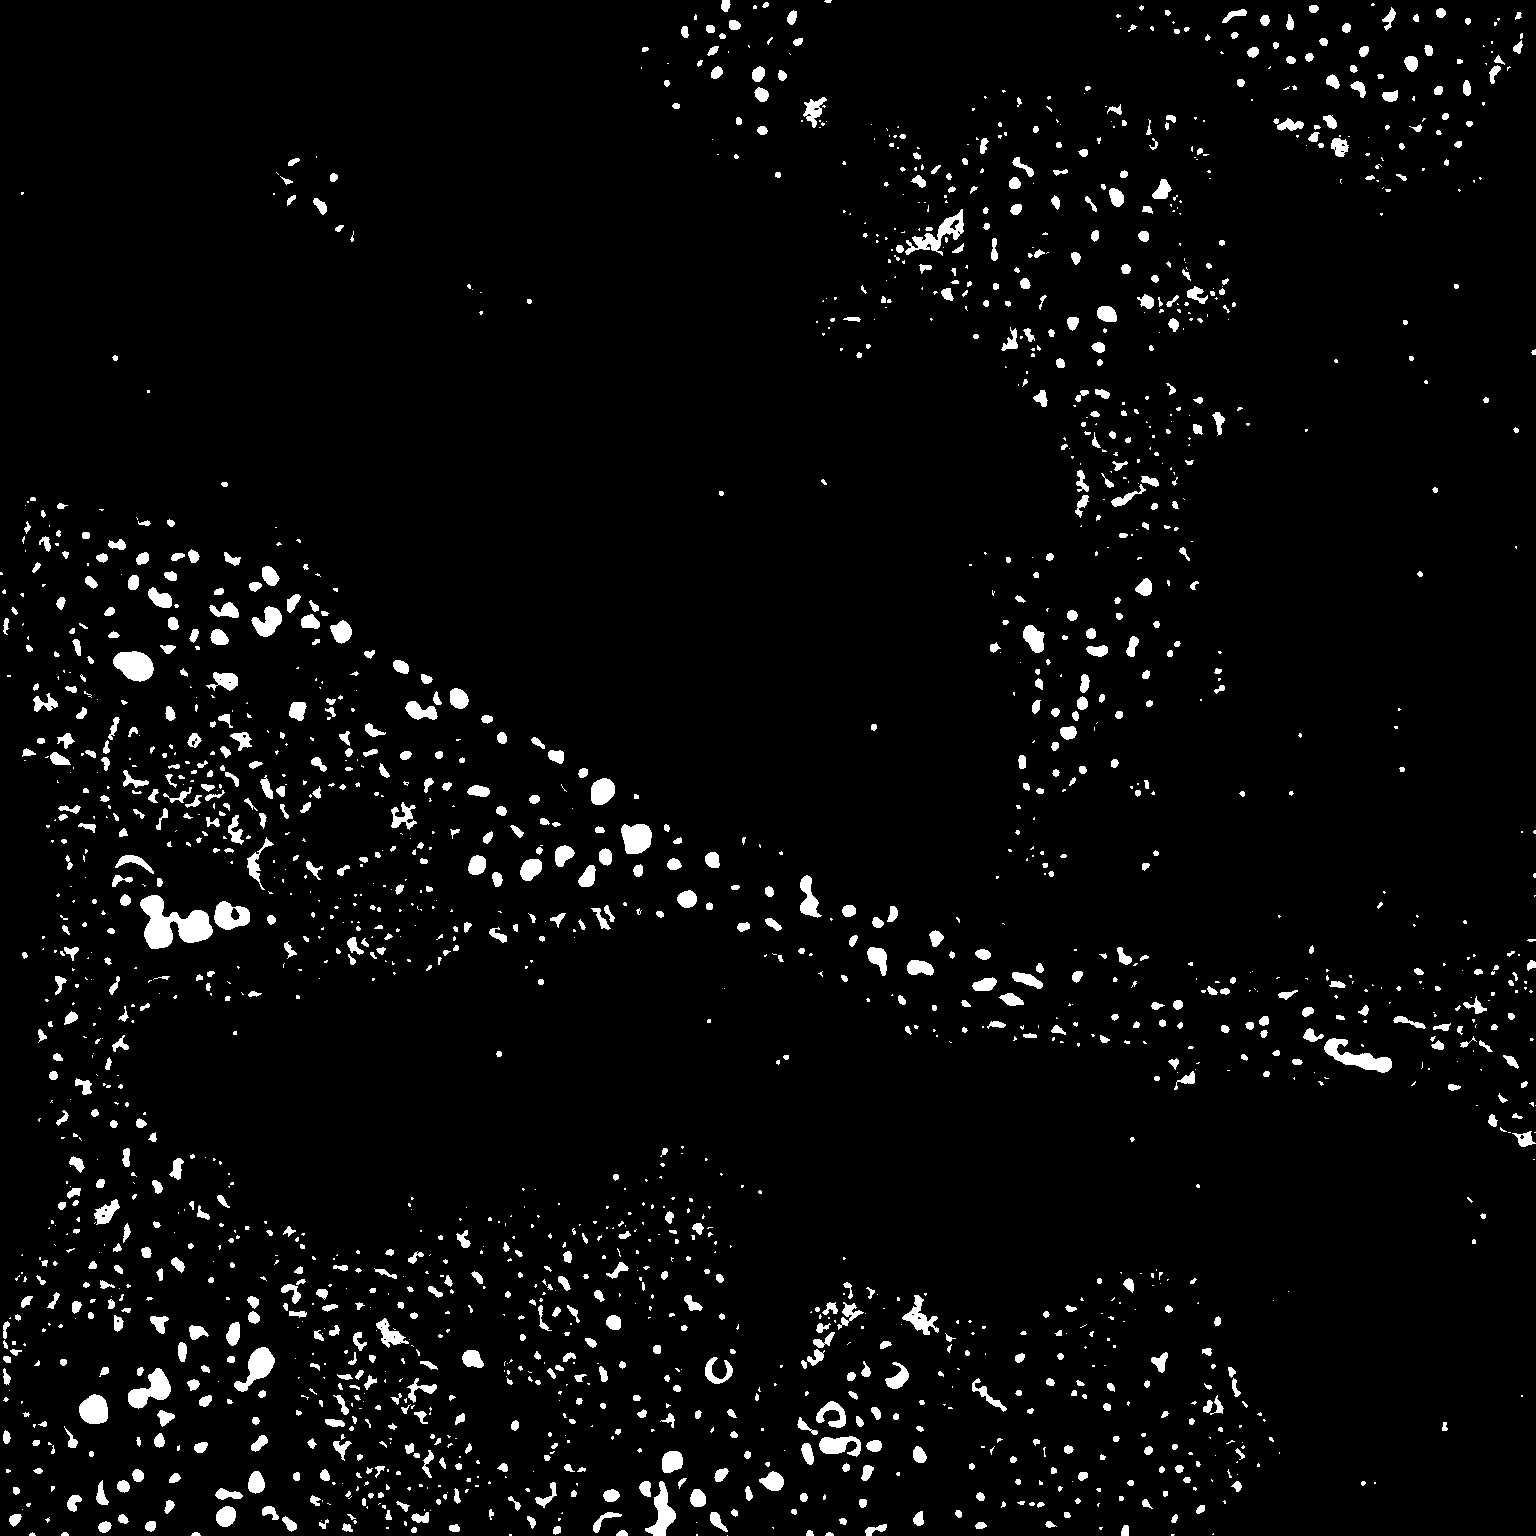
\includegraphics[width=0.3\textwidth]{figs/ch4figs/image_shortlisting/local/MidGrey_p0_w15_HML_4C=0.png}}
	\subcaptionbox{MidGrey thresholding with a subtraction constant of 5}{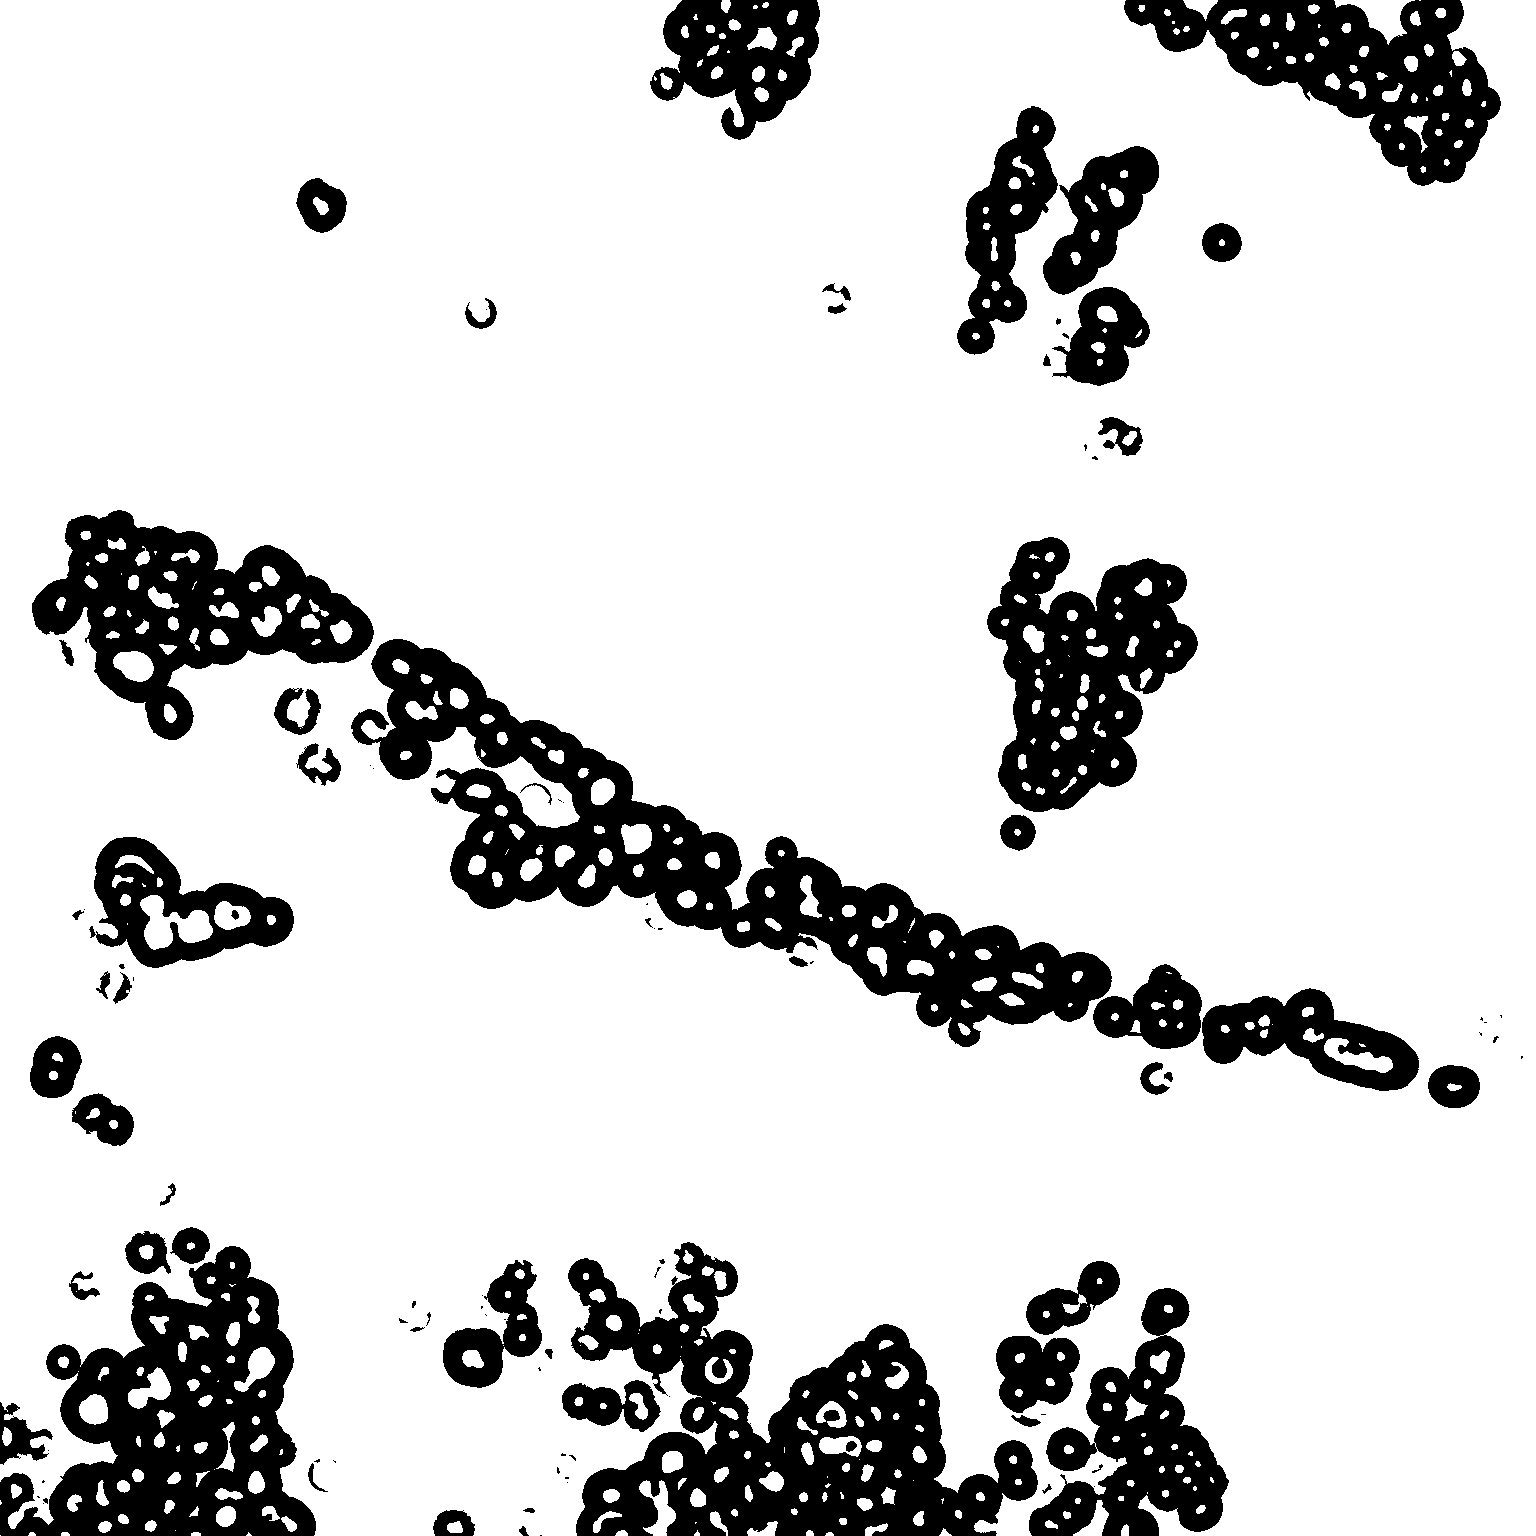
\includegraphics[width=0.3\textwidth]{figs/ch4figs/image_shortlisting/local/MidGrey_p5_w15_HML_4C=0.png}}
	\caption[Showcase of the impact secondary parameter tuning can have on local thresholding methods.]{Showcase of the impact secondary parameter tuning can have on local thresholding methods. Bernsen and MidGrey are used in this showcase with both being applied to sample 2.}
	\label{fig:local_param_tuning}
\end{figure}

\clearpage
\section{Visual analysis}\label{sec:visual_analysis}
With the global and local thresholding methods shortlisted, the performance of the AHT method can be evaluated against the shortlisted methods. This evaluation will be performed through visual analysis of the thresholding outcomes with comparison to manually tuned Hysteresis thresholding acting as the ``ground truth''. The motivation is that humans are more capable of inferring if the correct structures have been labelled as foreground in the thresholding outcomes although this does introduce a measure of bias thus making this not a true ground truth but rather an approximation of the structures a humans might subjectively try to include as foreground in the image. The ranking of the thresholding methods performance, compared to the manually tuned Hysteresis thresholding, will be designated by a value ranging from $0$ to $5$ with the implication of each rank score detailed in Table \ref{tab:rank_table}.
\paragraph{Sample images:} There is a total of three samples evaluated against with each presenting the lysosome, autophagosome and mitochondria organelle structures under different colour channels as shown in Figure \ref{fig:raw_samples_rgb}. Red represents the mitochondria, green represents the autophagosomes, and blue represents the lysosomes but the overlaying of multiple colour channels can make differentiation between the structures challenging. For this reason, the performance of the thresholding measures will be explored for each organelle structure type where the rankings for method groups (global thresholds, local thresholds, and AHT bias variations) will be scored for each sample. An overall ranking for each thresholding method will be presented for each organelle type with the top three performing methods of each group explored further. All thresholding outcome images are present in Appendix \ref{appen:visual_full_set}. 
\begin{table}
	\centering
	\begin{tabularx}{\linewidth}{|l|X|}
		\textbf{Rank}& \textbf{Rank Description}\\
		1 & The outcomes provided by this method are completely unusable \\
		2 & The outcomes present some under- or over-thresholding but the majority of structures are captured in the foreground \\
		3 & The outcomes are suitable for succeeding analysis although they still deviate from the manually tuned Hysteresis thresholding outcomes \\
		4 & The outcomes are equal to those achieved through manually tuned Hysteresis thresholding\\
		5 & The outcomes provided capture foreground structures while rejecting noise more effectively than the manually tuned Hysteresis thresholding (rejecting the false joining that Hysteresis is prone to is a contributor) \\
	\end{tabularx}
	\caption{Table of the rankings with each ranks associated description}
	\label{tab:rank_table}
\end{table}


\begin{figure}
	\centering
	\subcaptionbox{Sample A}{\includegraphics[width=0.32\textwidth]{figs/ch4figs/visual_analysis/raw_samples/RGB_Con_2C=0.png}}
	\subcaptionbox{Sample B}{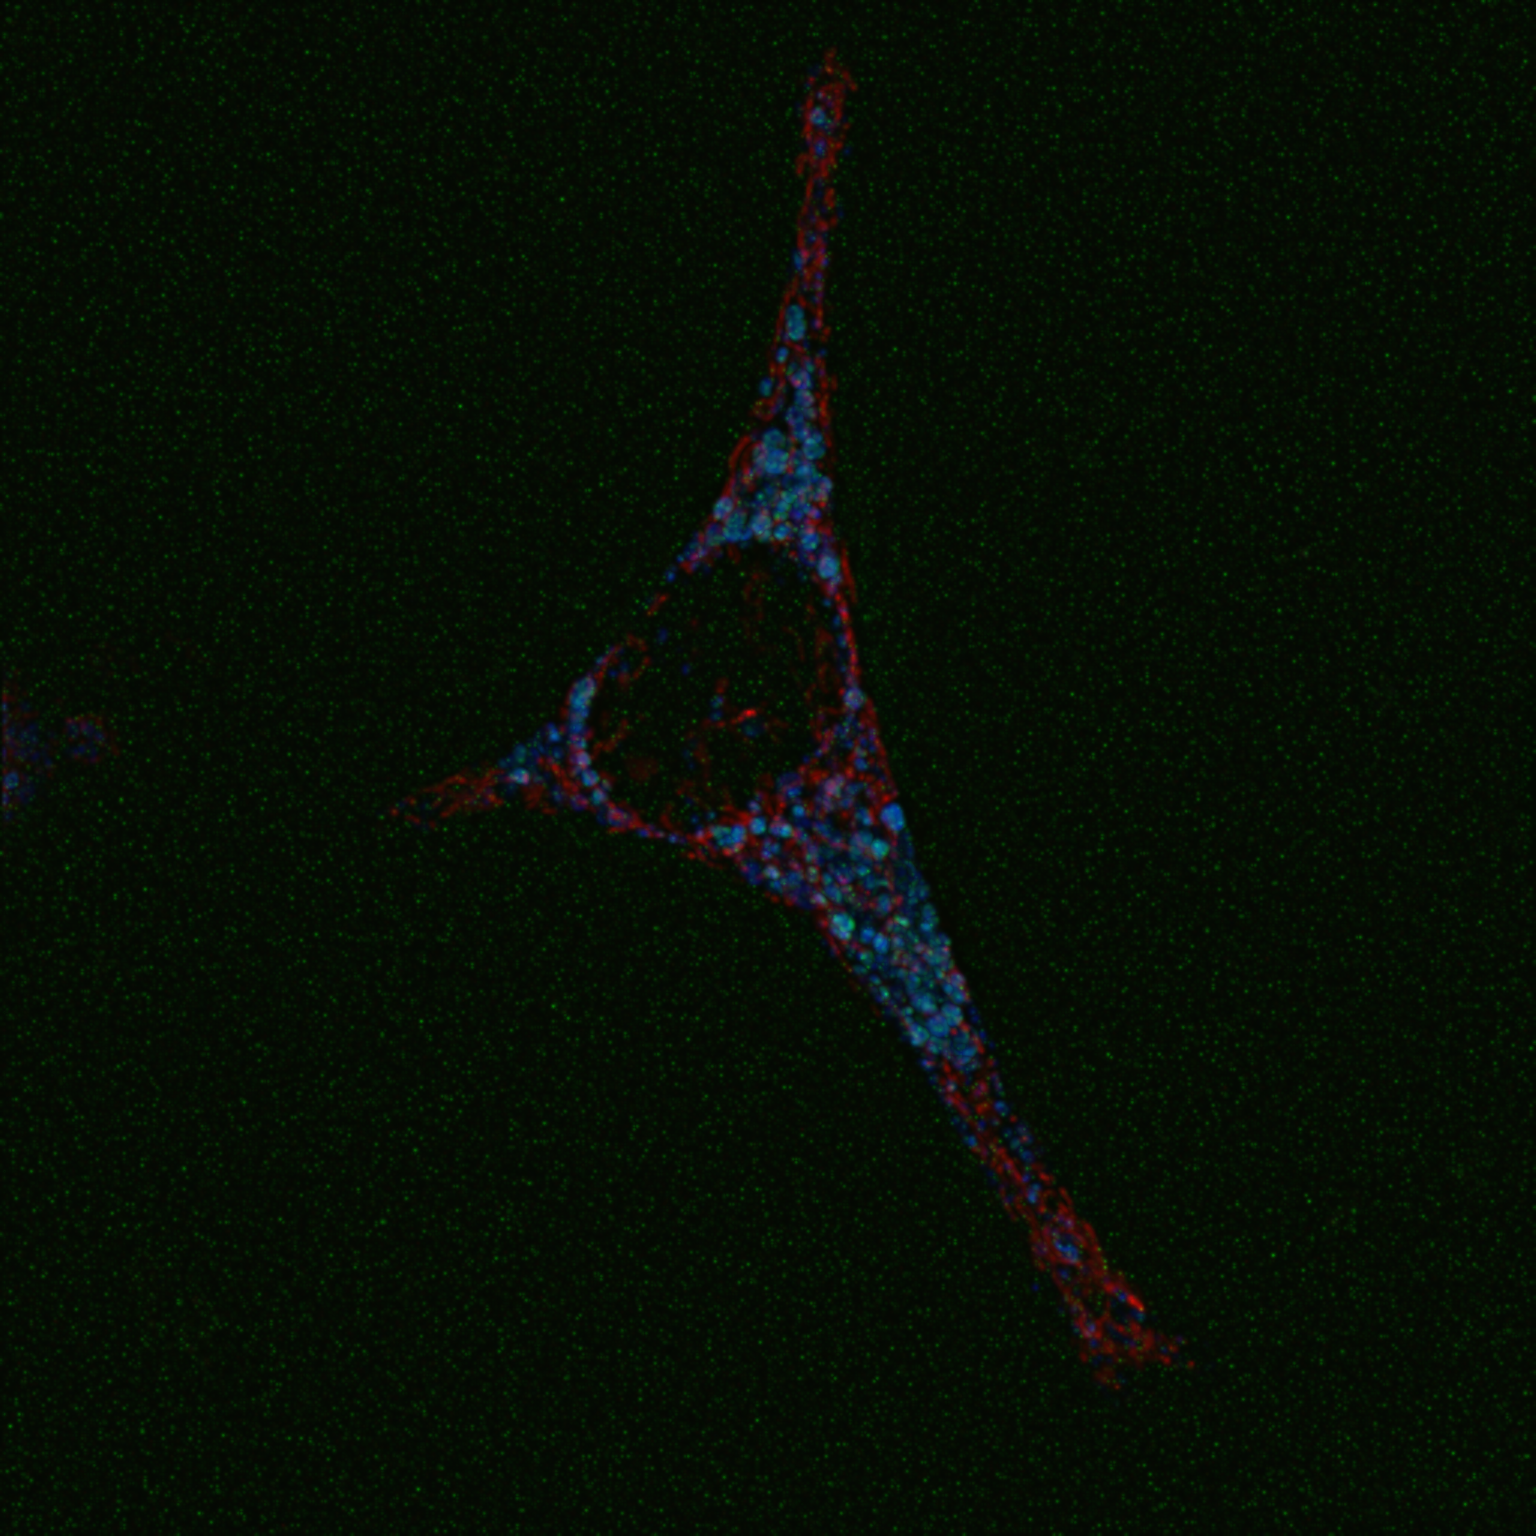
\includegraphics[width=0.32\textwidth]{figs/ch4figs/visual_analysis/raw_samples/RGB_LML_3C=0.png}}
	\subcaptionbox{Sample C}{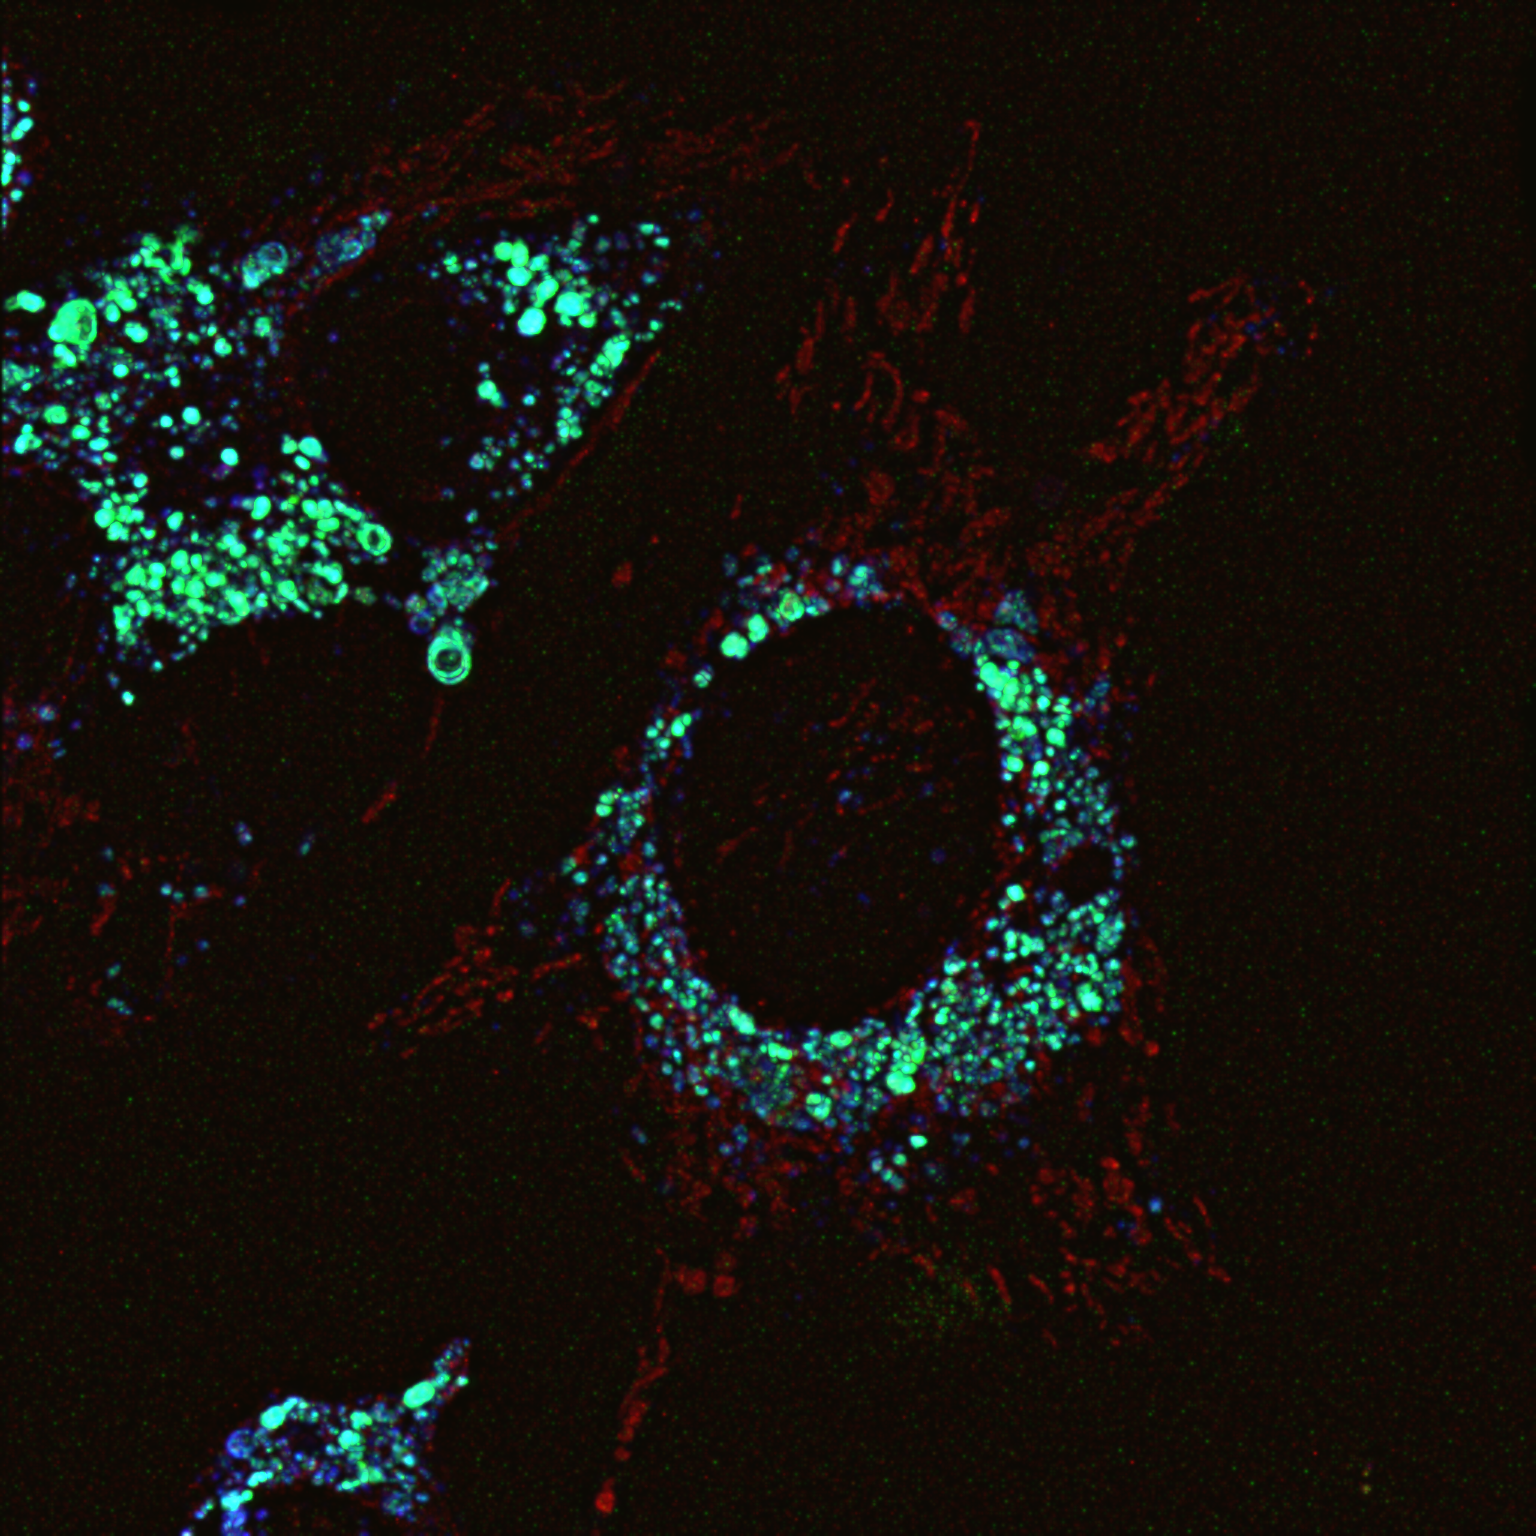
\includegraphics[width=0.32\textwidth]{figs/ch4figs/visual_analysis/raw_samples/RGB_LML_4C=1.png}}
	\caption[MIP sample images for the samples A-C where the organelle colour channels have been overlaid.]{MIP sample images for the samples A-C where the organelle colour channels have been overlaid. The lysosomes are represented by the blue channel, the autophagosomes are represented by the green channel, and the mitochondria are represented by the red channel.}
	\label{fig:raw_samples_rgb}
\end{figure}
\FloatBarrier
\subsection{Lysosome structures}
The lysosome structure images are presented in Figure \ref{fig:lysosome_raw} where the original MIP intensity images are shown along with the binary Hysteresis images for each sample. For each of these sample images, the accompanying Hysteresis threshold images are the foreground structures approximated through manual parameter tuning. \paragraph{Sample A:} Showcases foreground structures with high intensities that strongly contrast against the background but said background contains a large quantity of non-zero intensity noise and artefacts that could disrupt certain methods. \paragraph{Sample B:} Showcases foreground structures against a background containing little to no noise and, despite the maximum intensities for the majority of these structures being less than that of Sample A, the high contrast due to the low presence of noise could be ideal for many thresholding methods.\paragraph{Sample C:} Balanced between Sample A and Sample B, this sample possesses relatively high intensities for the foreground structures but with the presence of overlapping lower-intensity structure volumes, either belonging to out-of-focus structures or the structural volumes with low fluorophore concentrations, presents a challenge for confident differentiation for both manual and automatic thresholding methods.

\begin{figure}[ht!]
	\subcaptionbox{Sample A in Viridis}{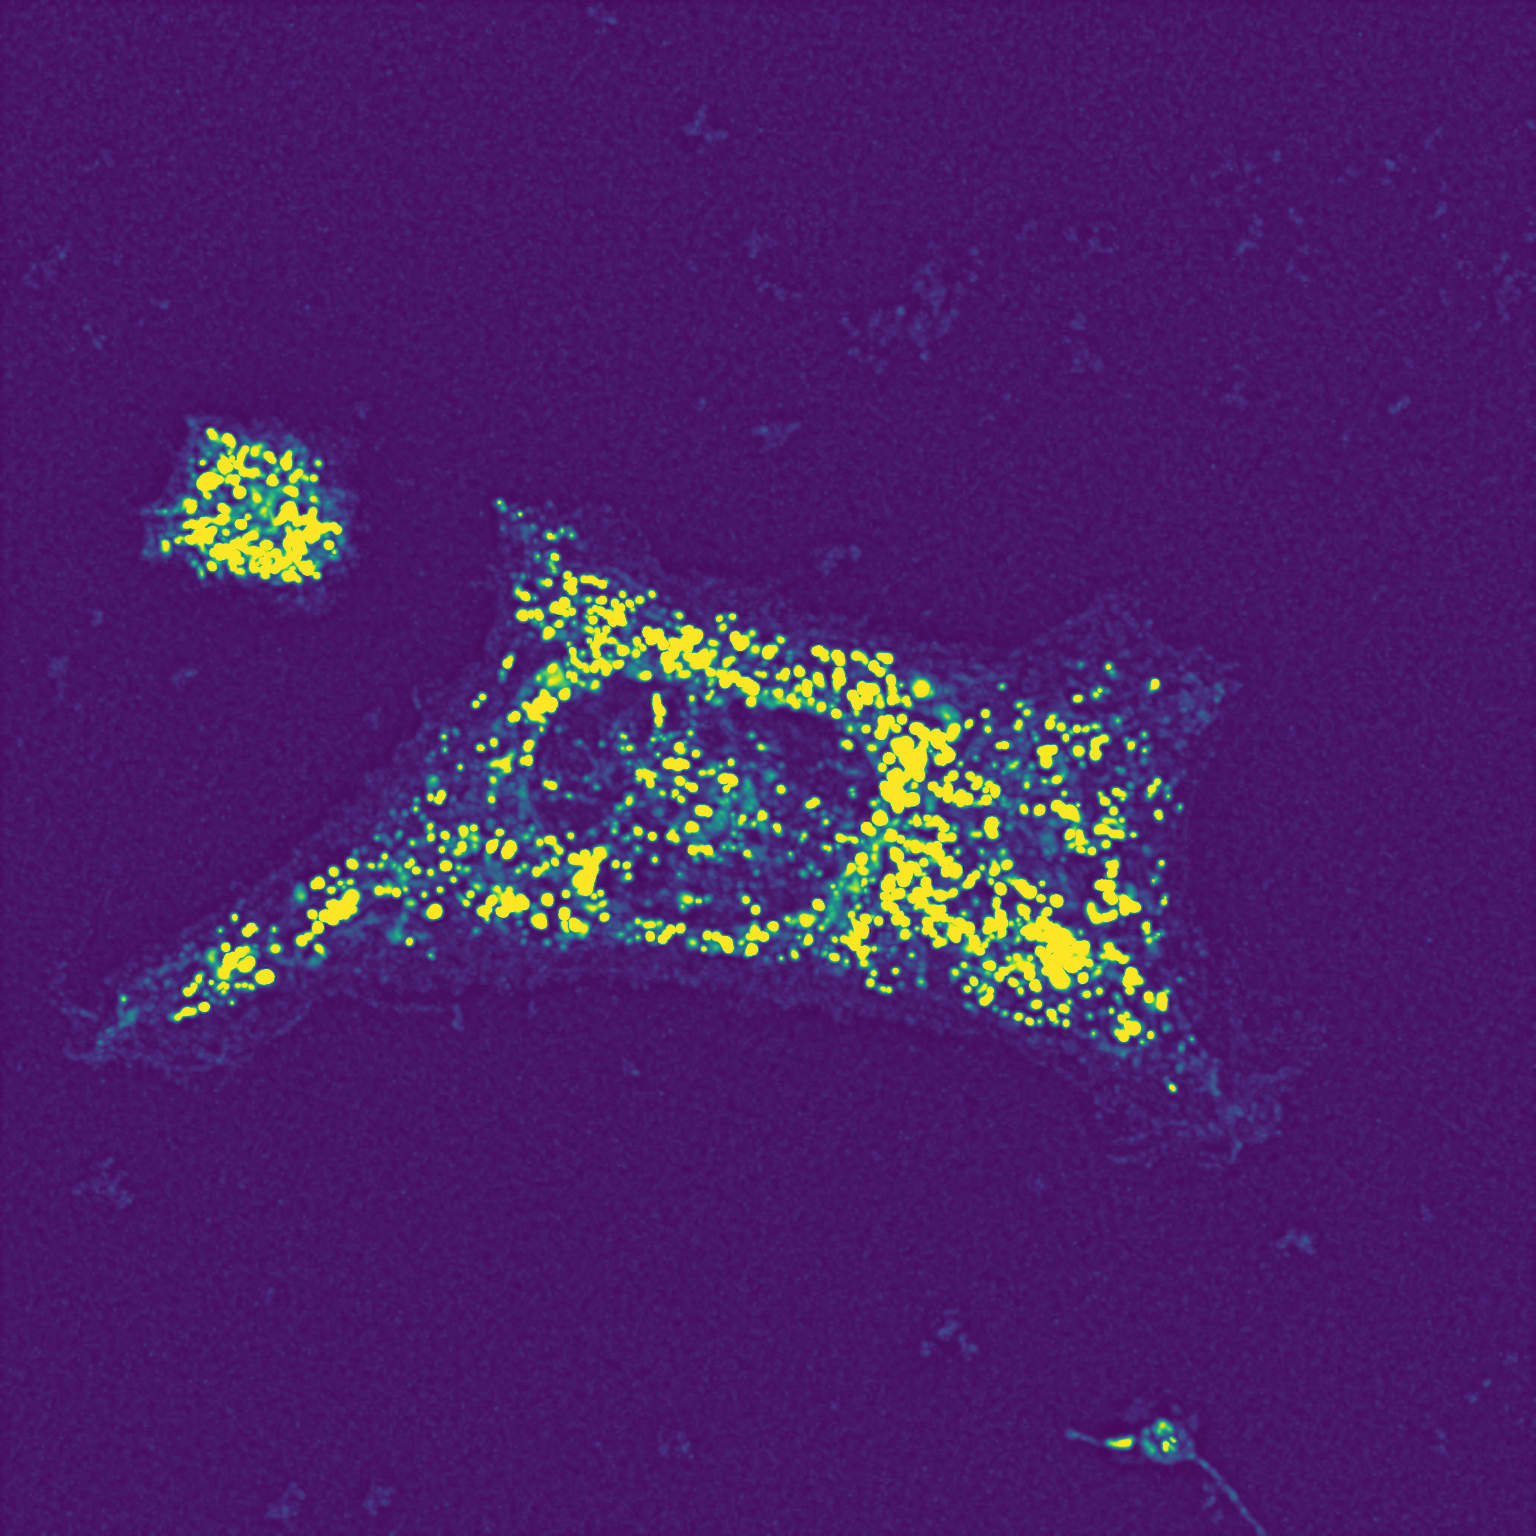
\includegraphics[width=0.32\textwidth]{figs/ch4figs/visual_analysis/raw_samples/MAX_Con_2C=0.png}}
	\subcaptionbox{Sample B in Viridis}{
\includegraphics[width=0.32\textwidth]{figs/ch4figs/visual_analysis/raw_samples/MAX_LML_3C=0.png}}
	\subcaptionbox{Sample C in Viridis}{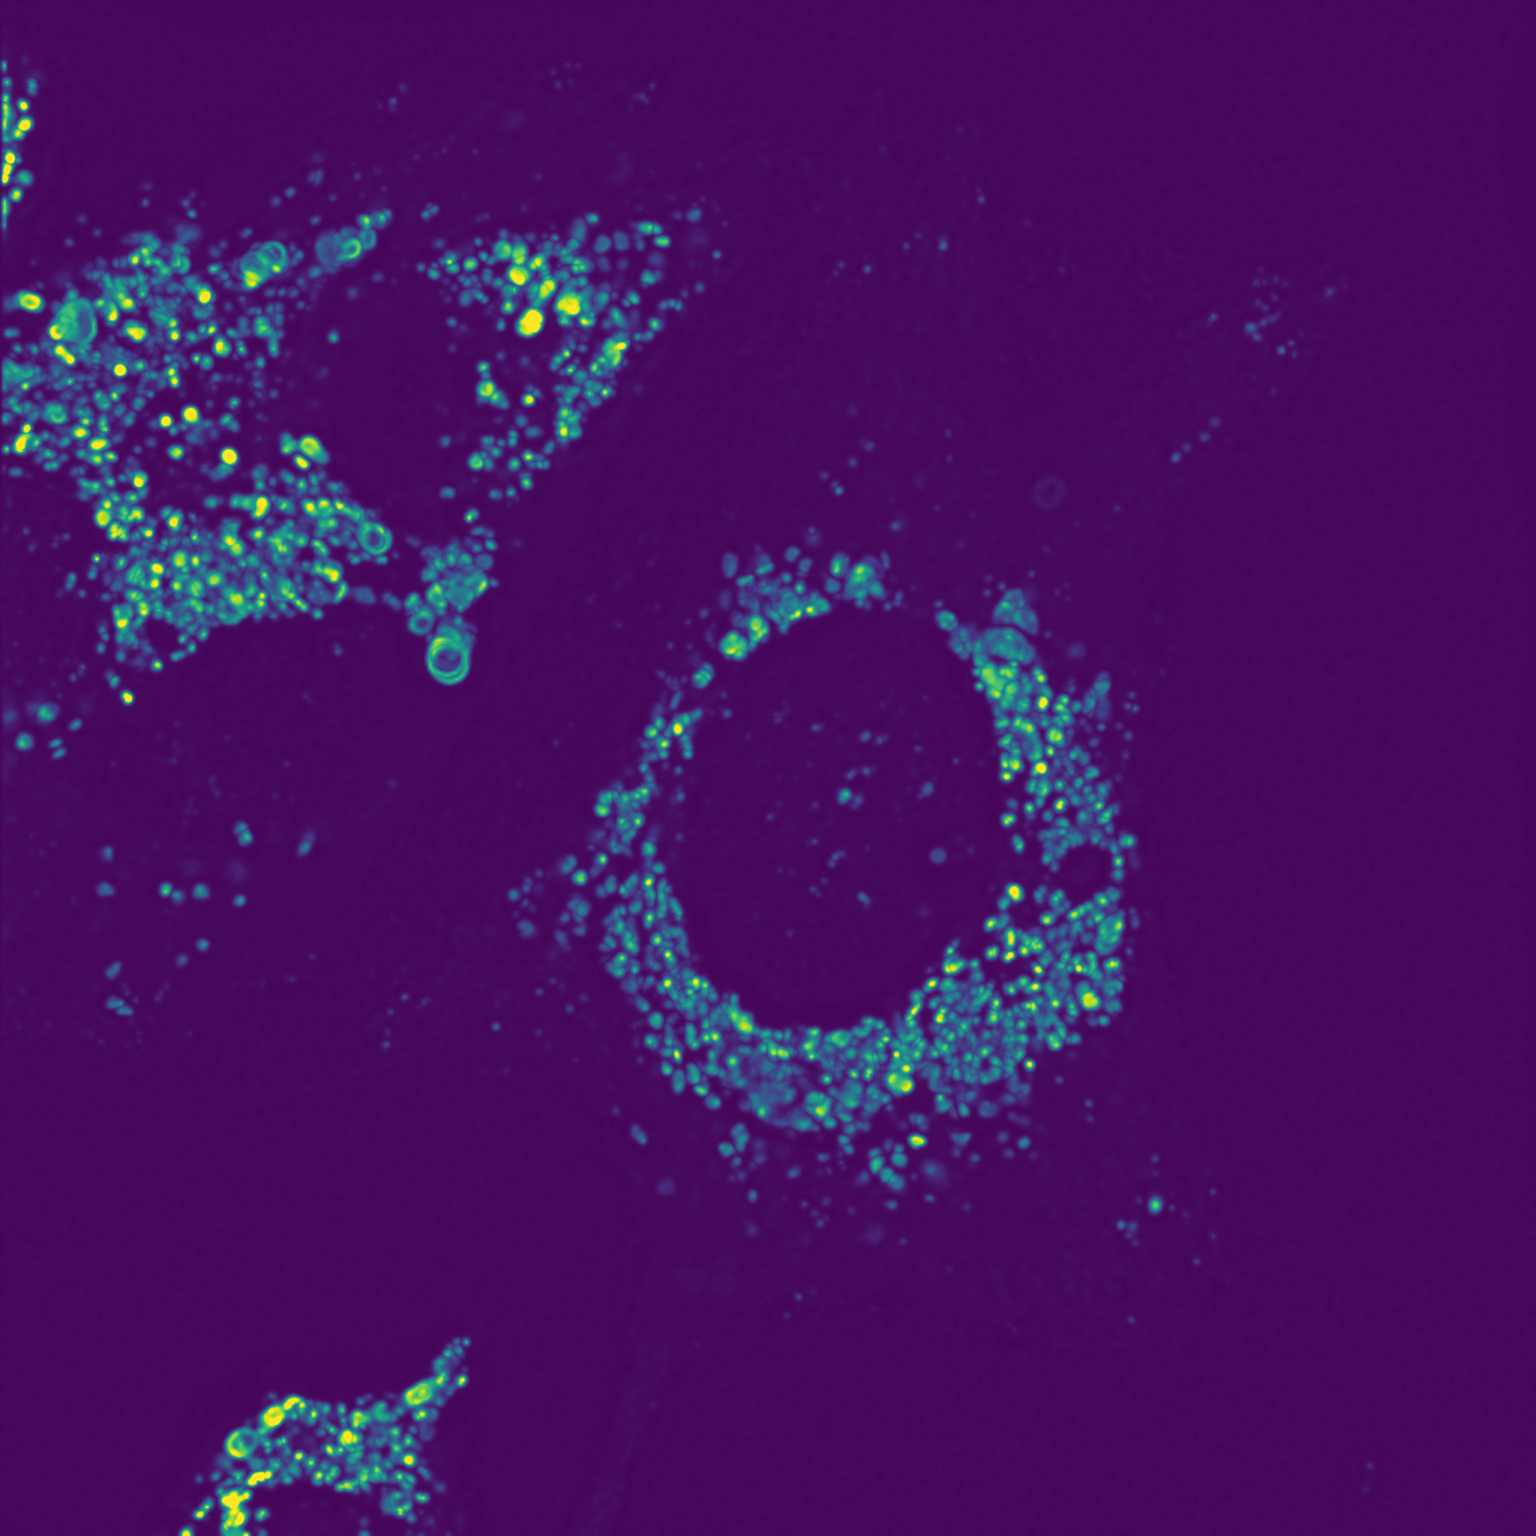
\includegraphics[width=0.32\textwidth]{figs/ch4figs/visual_analysis/raw_samples/MAX_LML_4C=0.png}}
	\subcaptionbox{Sample A Hysteresis thresholding}{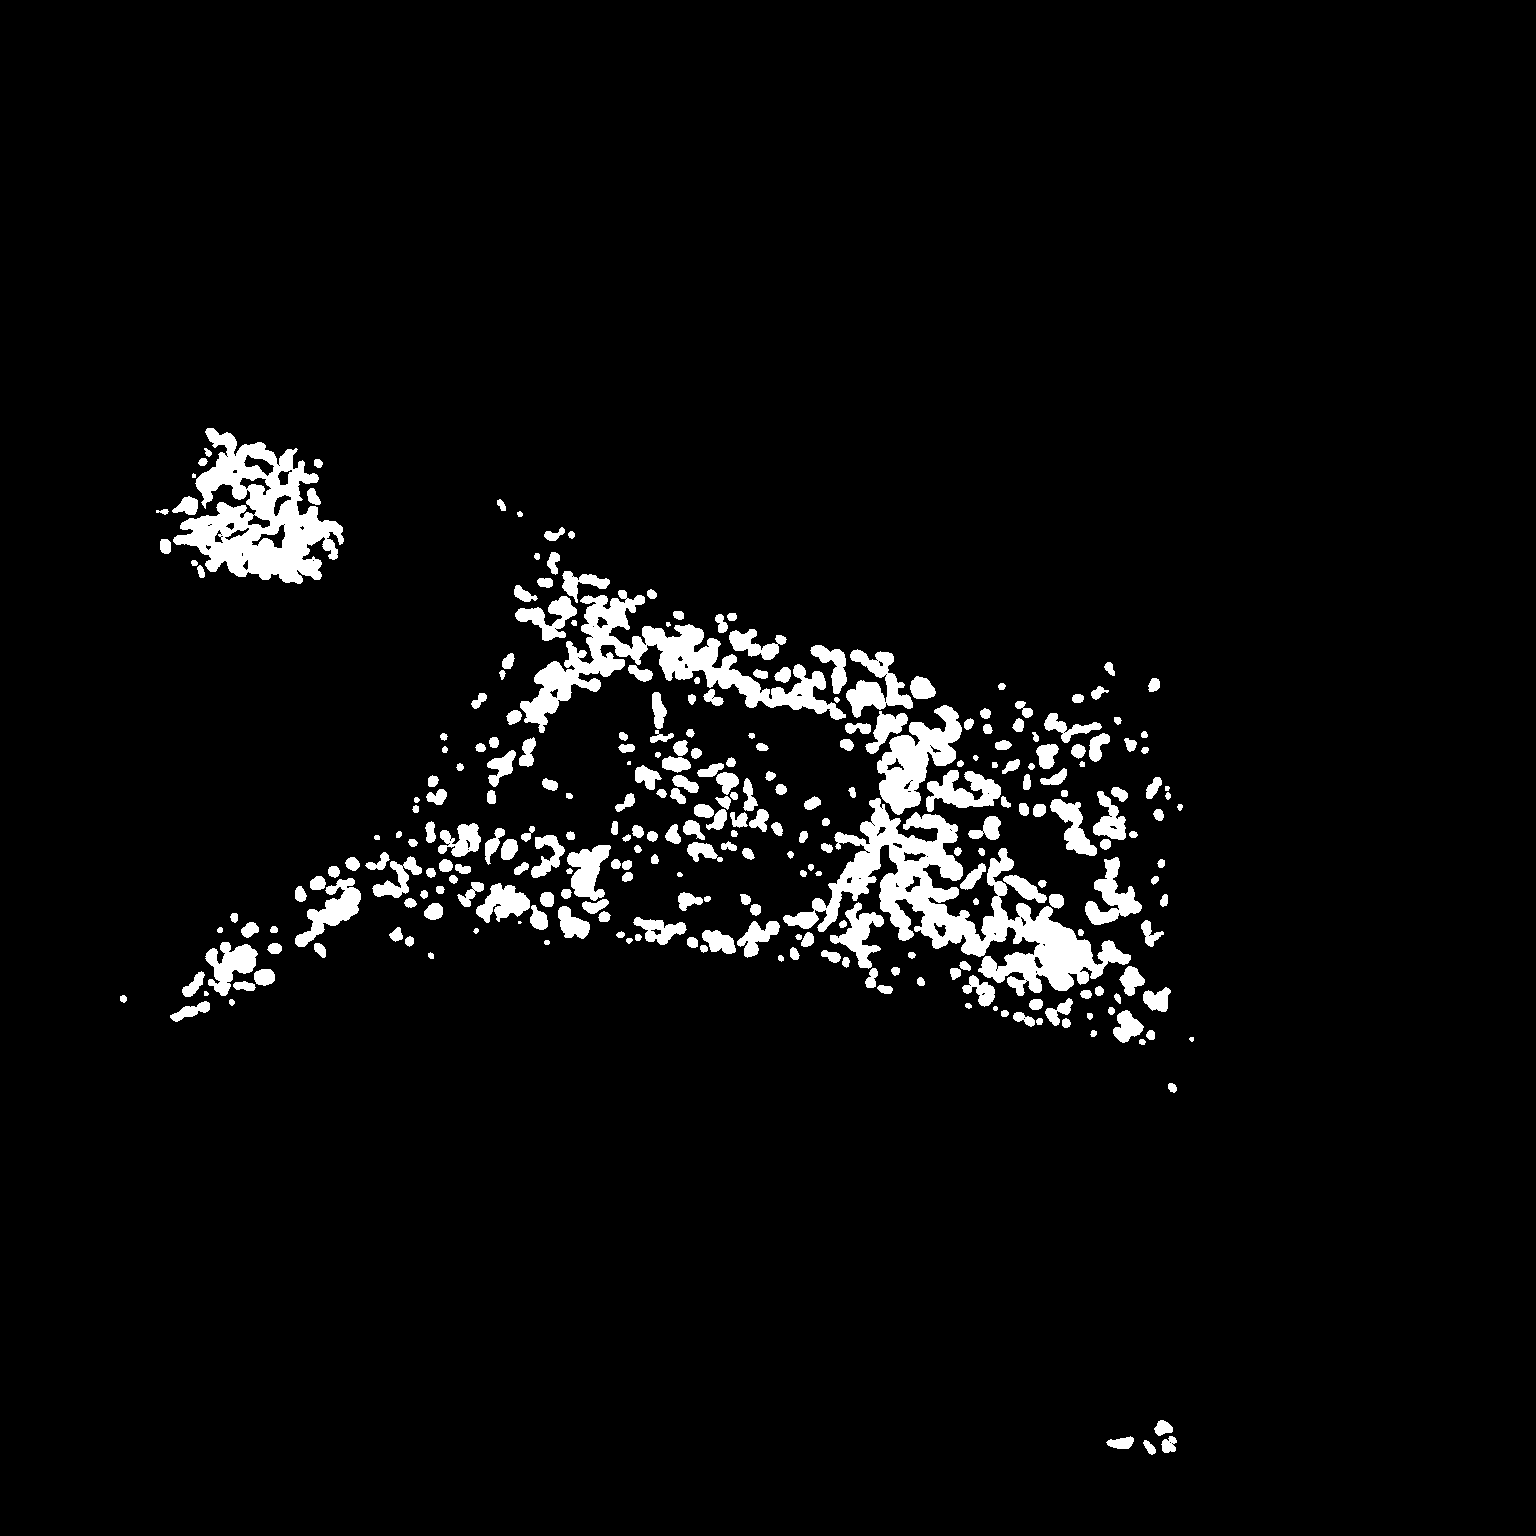
\includegraphics[width=0.32\textwidth]{figs/ch4figs/visual_analysis/raw_samples/Hyst_Con_2C=0.png}}
	\subcaptionbox{Sample B Hysteresis thresholding}{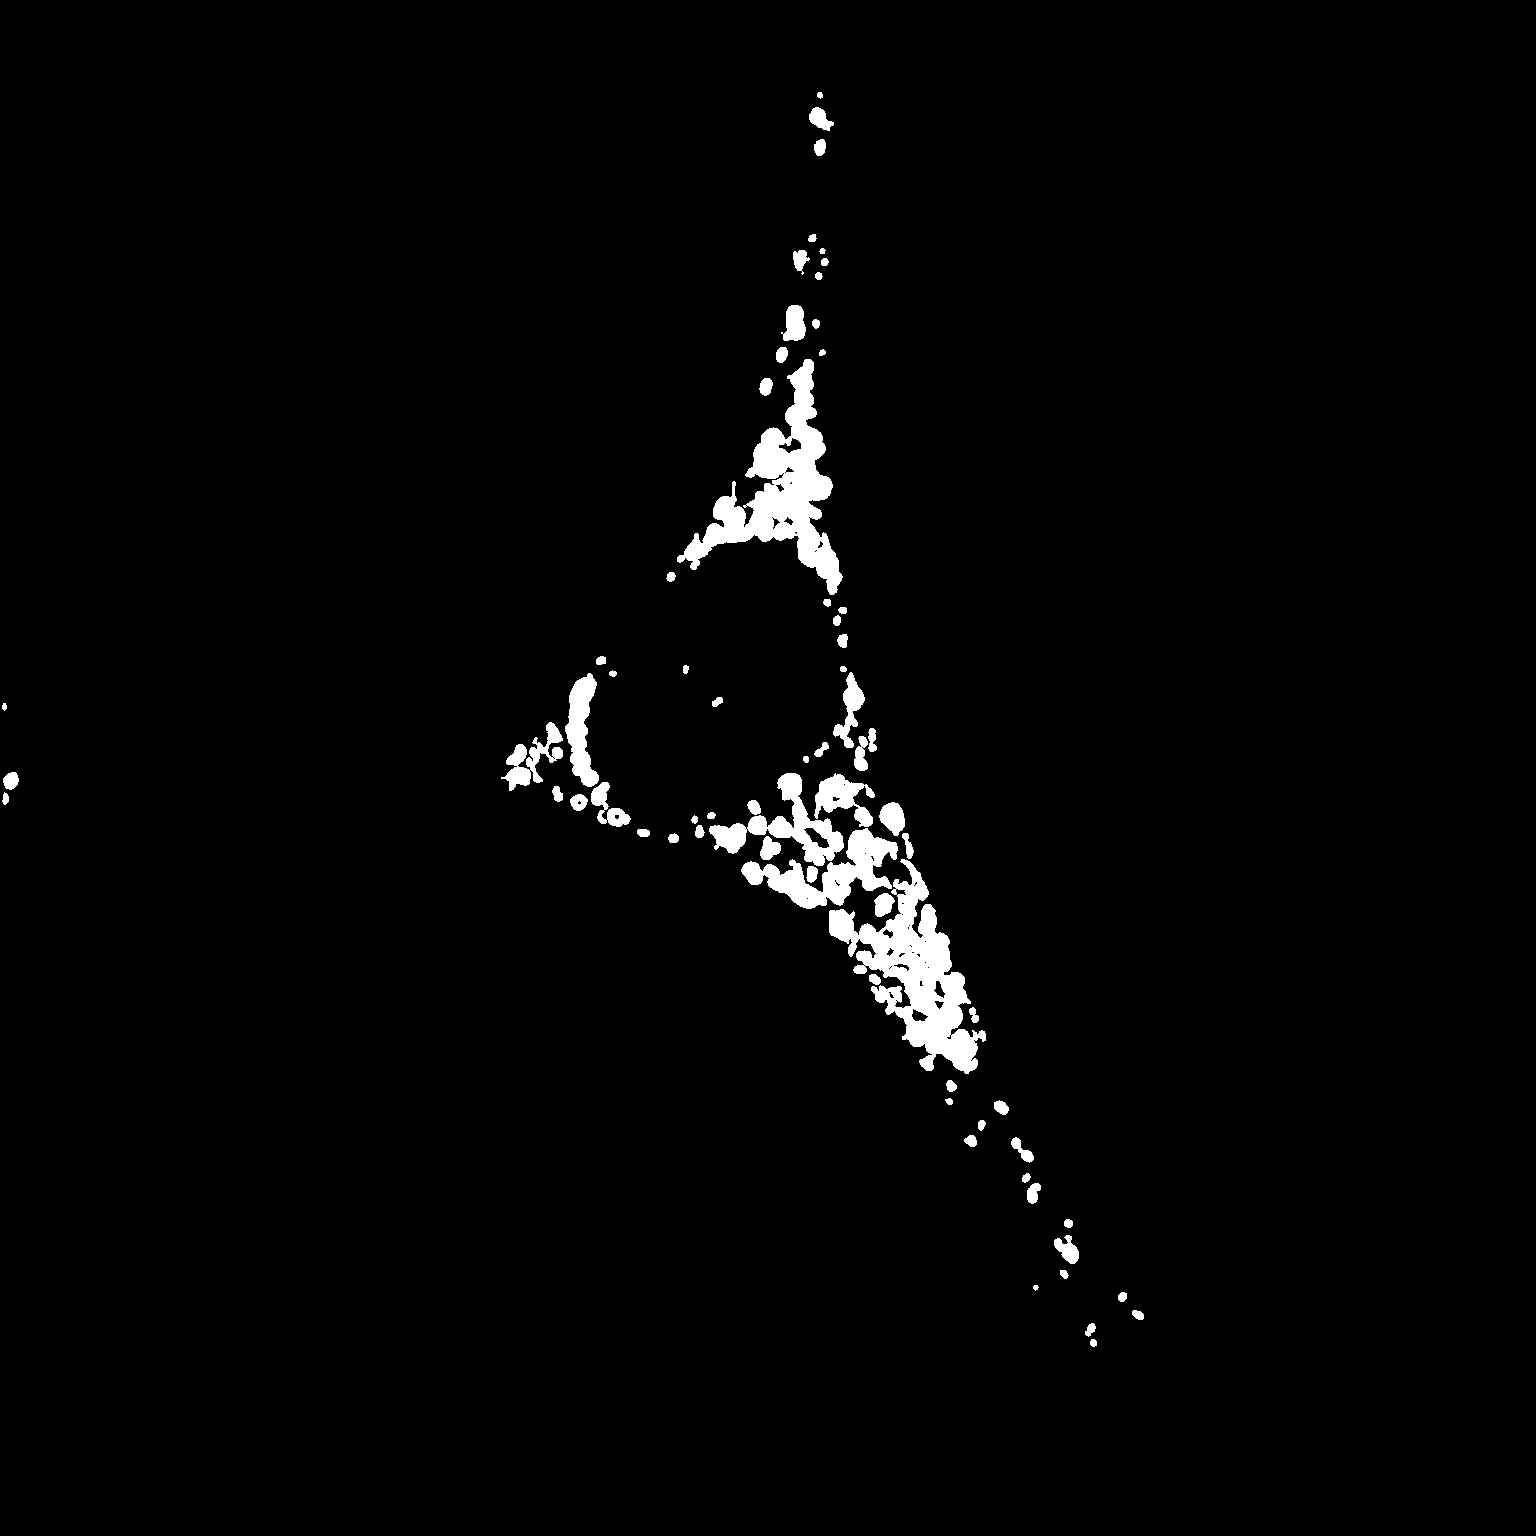
\includegraphics[width=0.32\textwidth]{figs/ch4figs/visual_analysis/raw_samples/Hyst_LML_3C=0.png}}
	\subcaptionbox{Sample C Hysteresis thresholding}{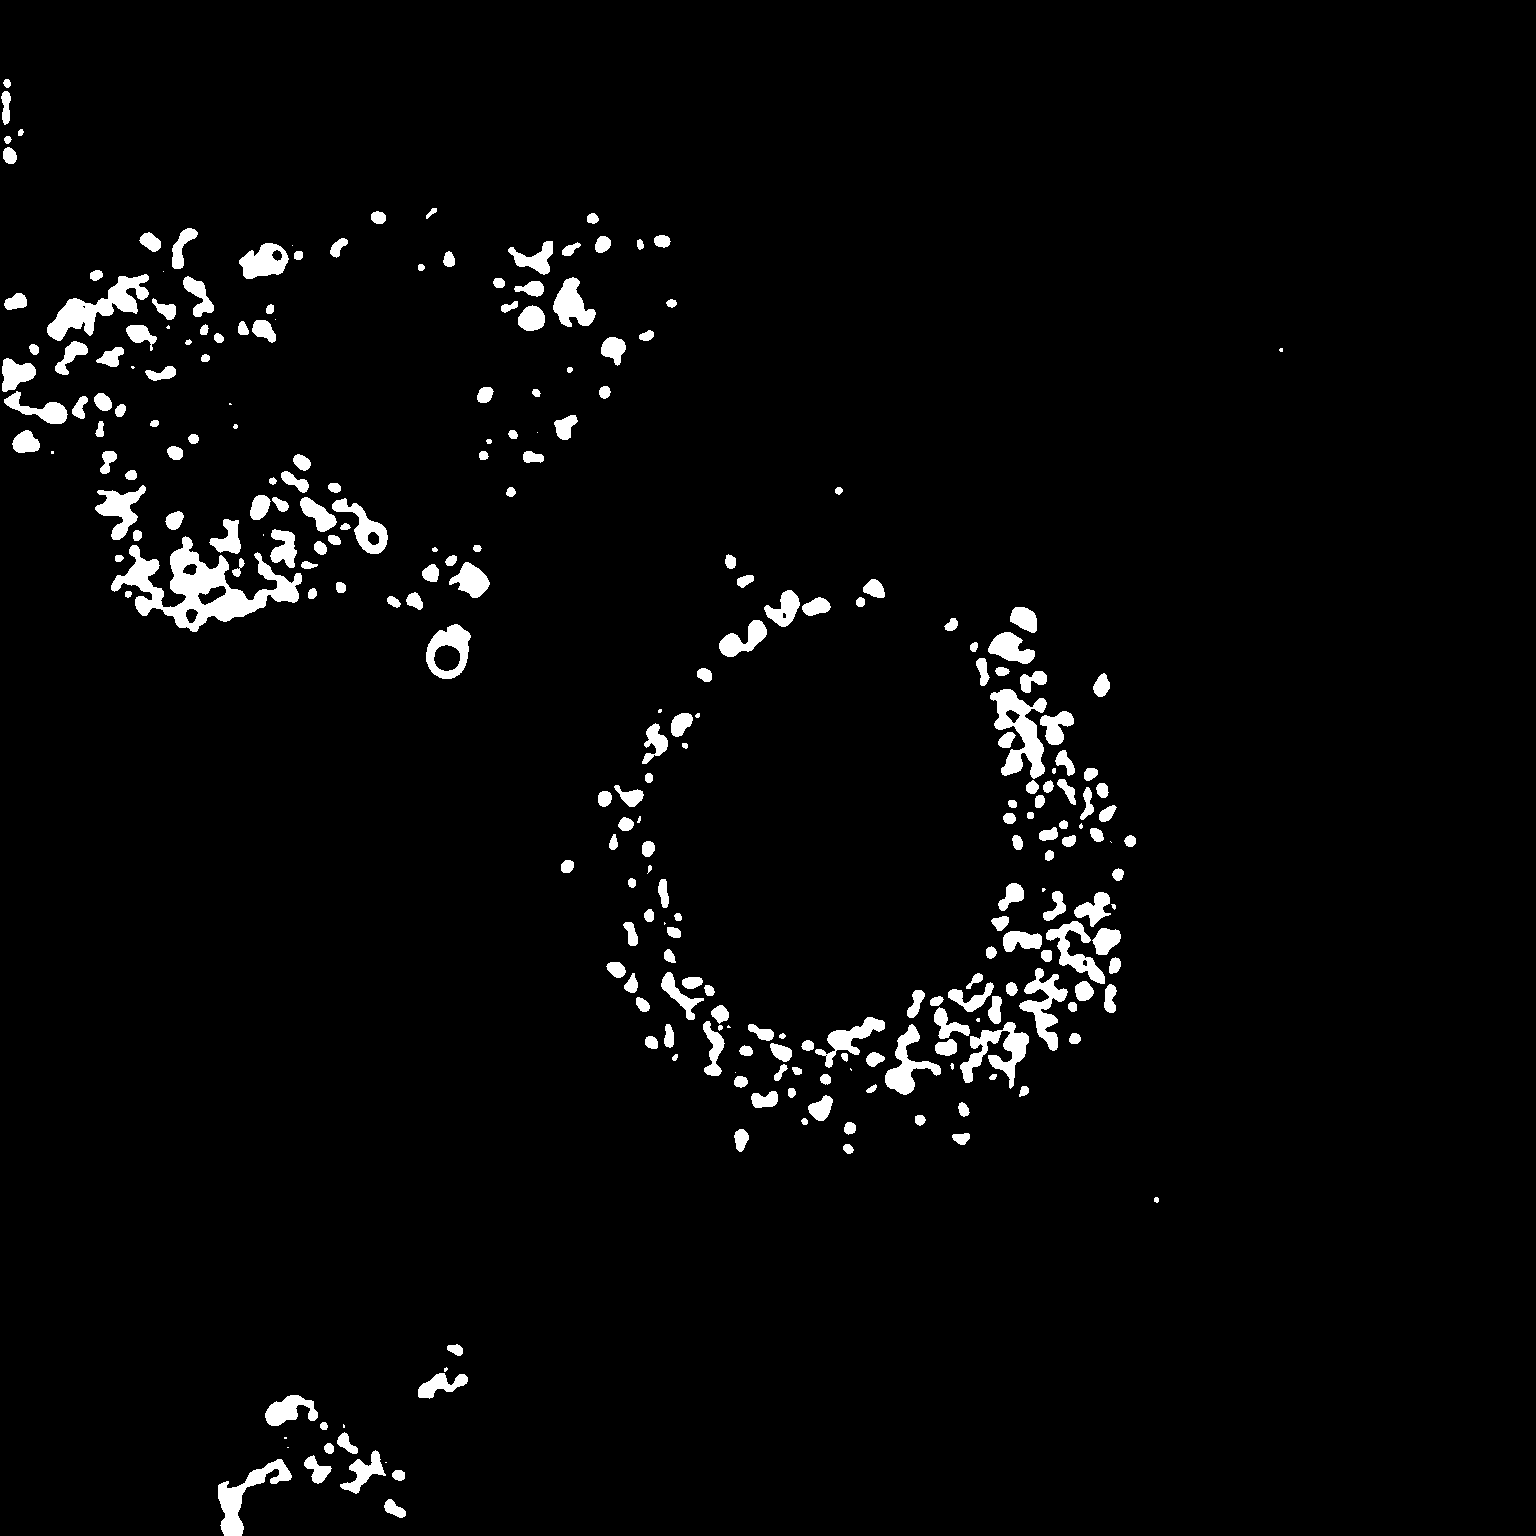
\includegraphics[width=0.32\textwidth]{figs/ch4figs/visual_analysis/raw_samples/Hyst_LML_4C=0.png}}
	\caption[Showcase of the lysosome evaluation samples as MIP images.]{Showcase of the lysosome evaluation samples as MIP images. The first row shows the pre-processed images, prior to any thresholding, in the viridis colourmap. The second row shows the same samples after manually tuned Hysteresis thresholding has been applied.}
	\label{fig:lysosome_raw}
\end{figure}
\FloatBarrier
\subsubsection{Global thresholding methods}
For the lysosome structures the top three global thresholding methods are Moments, IsoData and Otsu based on the mean rankings in Table \ref{tab:lyso_global_ranks}.
\begin{table}[hb!]
	\centering
	\begin{tabular}{|c|c|c|c|c|}
		\hline
		\textbf{Method} & \textbf{Sample A} & \textbf{Sample B} & \textbf{Sample C} & \textbf{Mean Rank} \\
		\hline
		Huang2 & 1 & 2 & 2 & 1.6 \\
		\hline
		IsoData & 4 & 3 & 3 & 3.3 \\
		\hline
		Li & 1 & 1 & 1 & 1 \\
		\hline
		MaxEntropy & 1 & 3 & 2 & 2 \\
		\hline
		Moments & 3 & 3 & 5 & 3.6 \\
		\hline
		Otsu & 4 & 3 & 3 & 3.3 \\
		\hline
		RenyiEntropy & 1 & 3 & 5 & 3 \\
		\hline
		Triangle & 1 & 2 & 2 & 1.6 \\
		\hline
		Yen & 1 & 3 & 5 & 3 \\
		\hline
	\end{tabular}
	\caption{Rankings for each of the global thresholding methods for the lysosome sample images}
	\label{tab:lyso_global_ranks}
\end{table}

\FloatBarrier
\paragraph{Moments}
The showcase of the Moments threshold outcomes is shown in Figure \ref{fig:lyso_moments} with the Moments threshold outcomes compared against the Hysteresis threshold outcomes in a red-green image for each sample. There are also binarized images for each sample of only the Moments threshold outcomes which matches the red colour channel in the red-green images. From this figure, it is observed that the Moments threshold and Hysteresis threshold outcomes for both samples A and B are very similar save for Moments having a few more foreground structures. Considering the greater low-intensity noise present in sample A, compared to the other samples, and the low average structural intensities for sample B this difference of a few structures is negligible since the Hysteresis thresholding baseline compared against is an imperfect ground truth due to the bias involved in it. The biggest deviation is for sample C where Moments separates structures that are joined in the Hysteresis threshold outcome but this joining is likely false, a flaw of Hysteresis thresholding, based on the intensity image of sample C in Figure \ref{fig:lysosome_raw}. For this reason, it is deemed that Moments thresholding outperforms Hysteresis thresholding for sample C.
\begin{figure}[h!]
	\subcaptionbox{Sample A overlay}{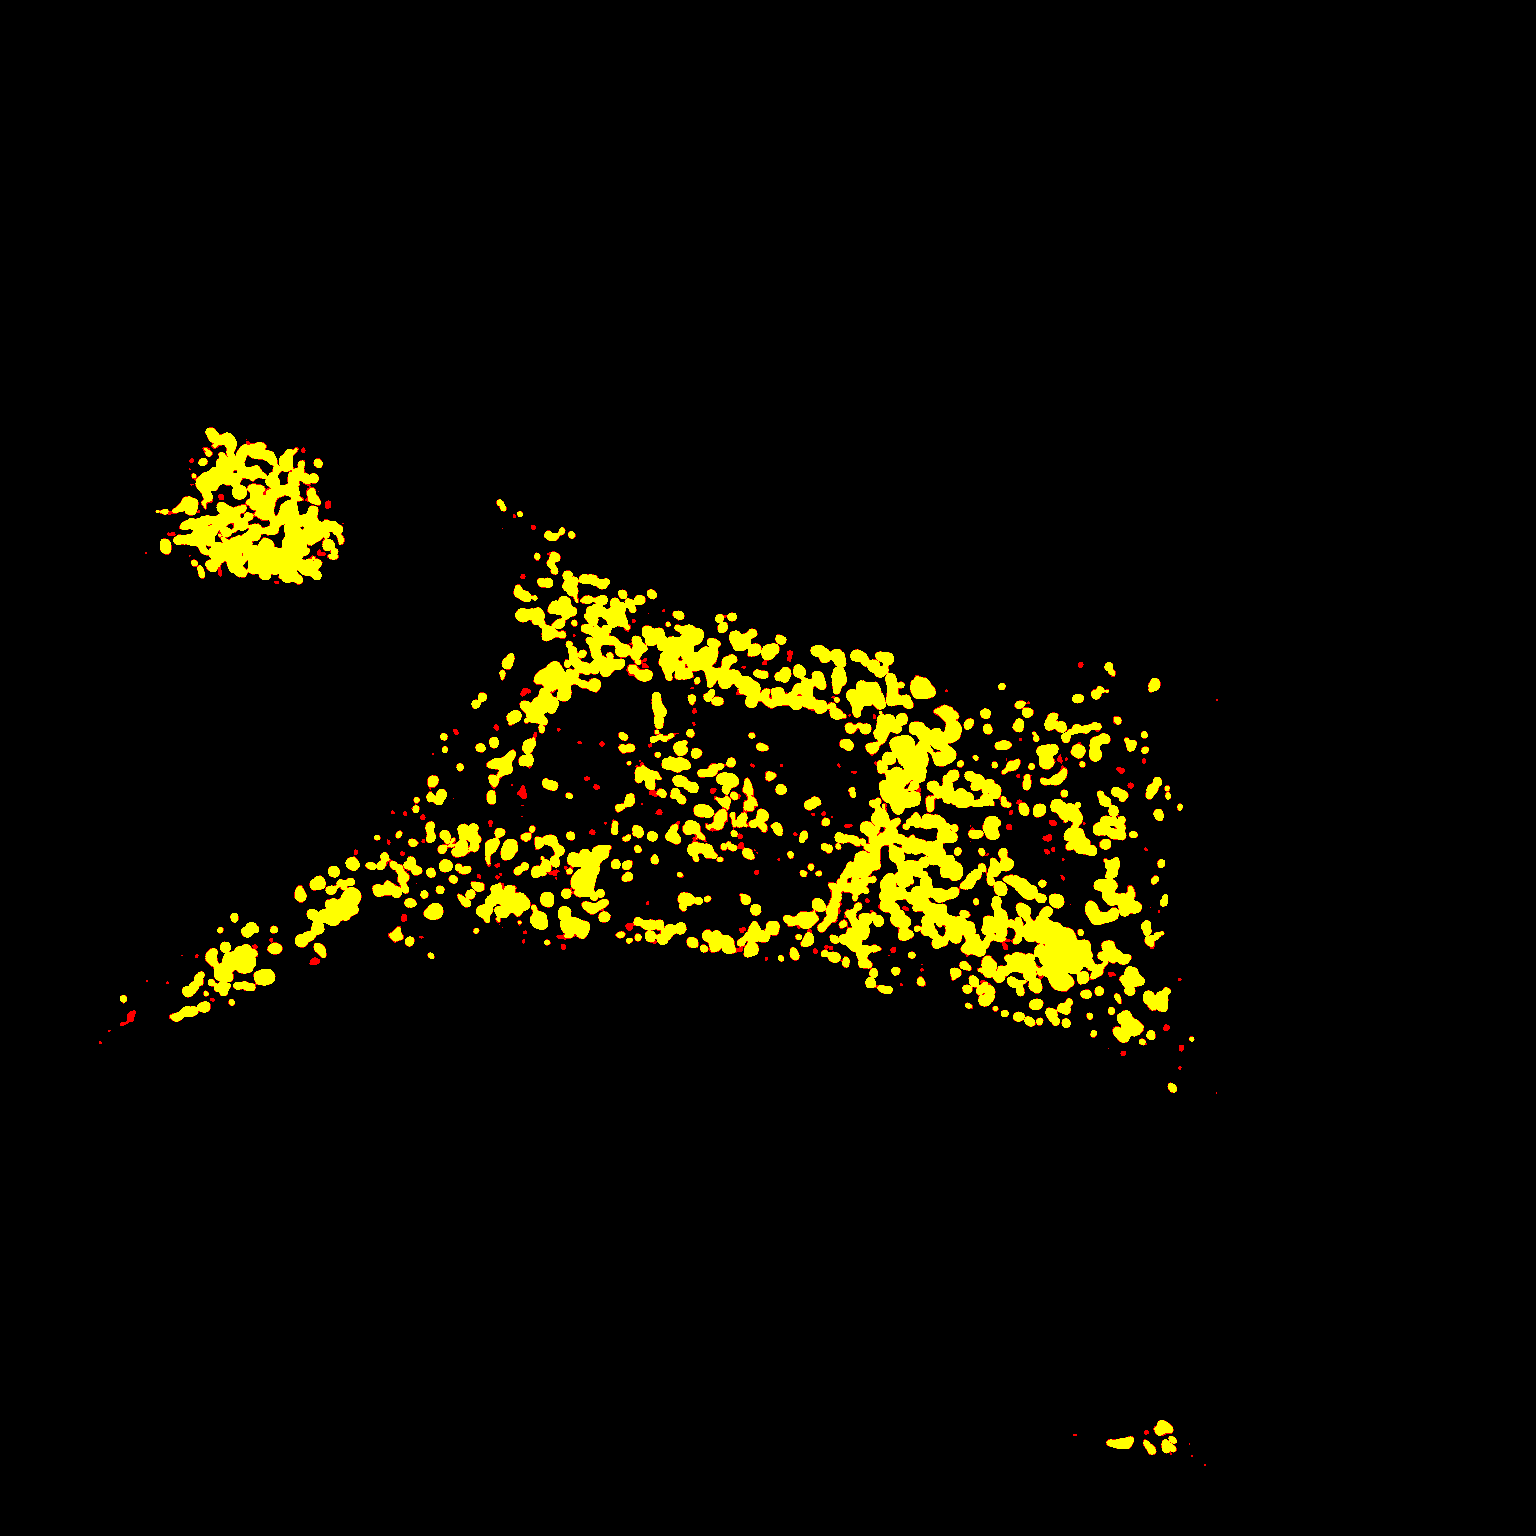
\includegraphics[width=0.32\textwidth]{figs/ch4figs/visual_analysis/global_outcomes/lyso/Moments_Con_2C=0.png}}
	\subcaptionbox{Sample B overlay}{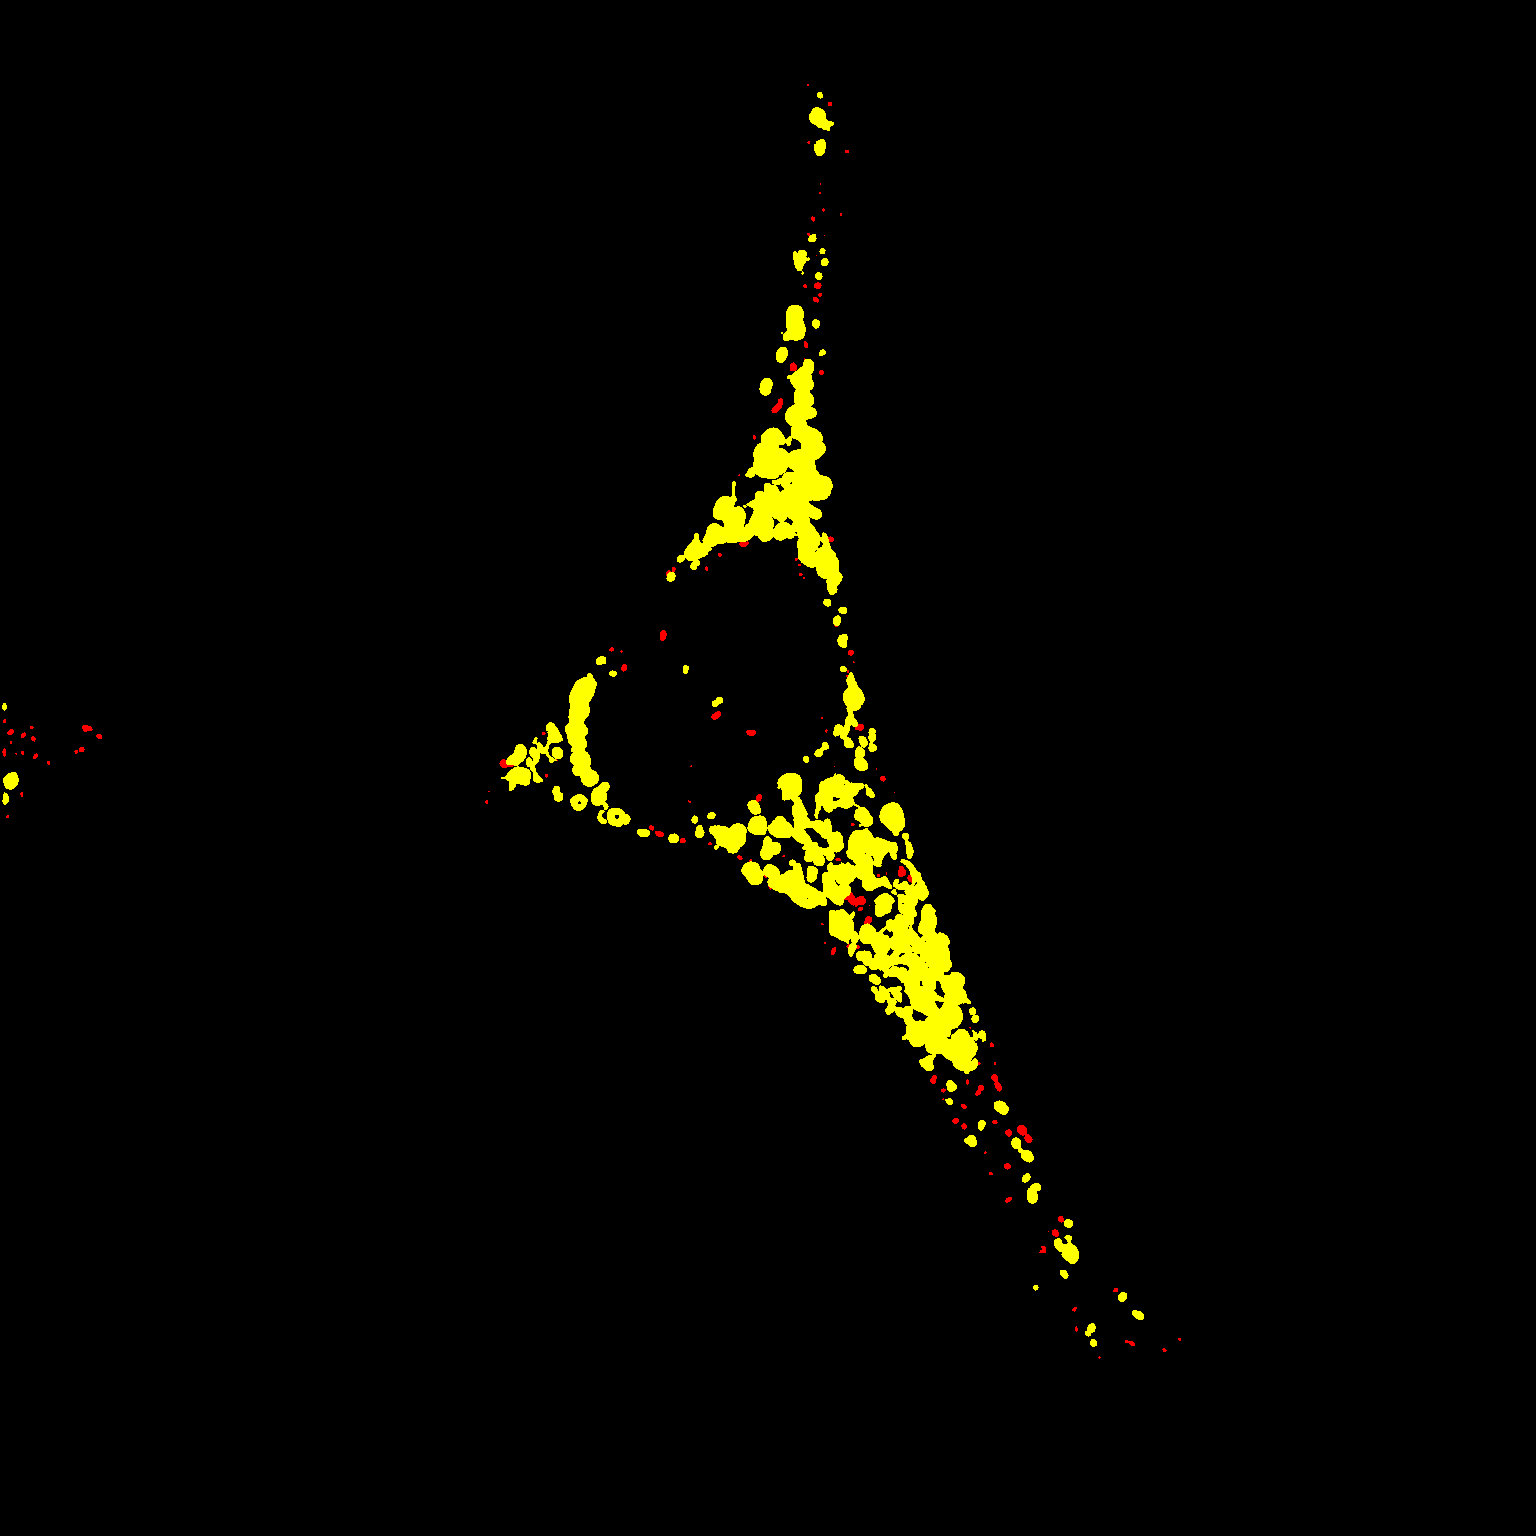
\includegraphics[width=0.32\textwidth]{figs/ch4figs/visual_analysis/global_outcomes/lyso/Moments_LML_3C=0.png}}
	\subcaptionbox{Sample C overlay}{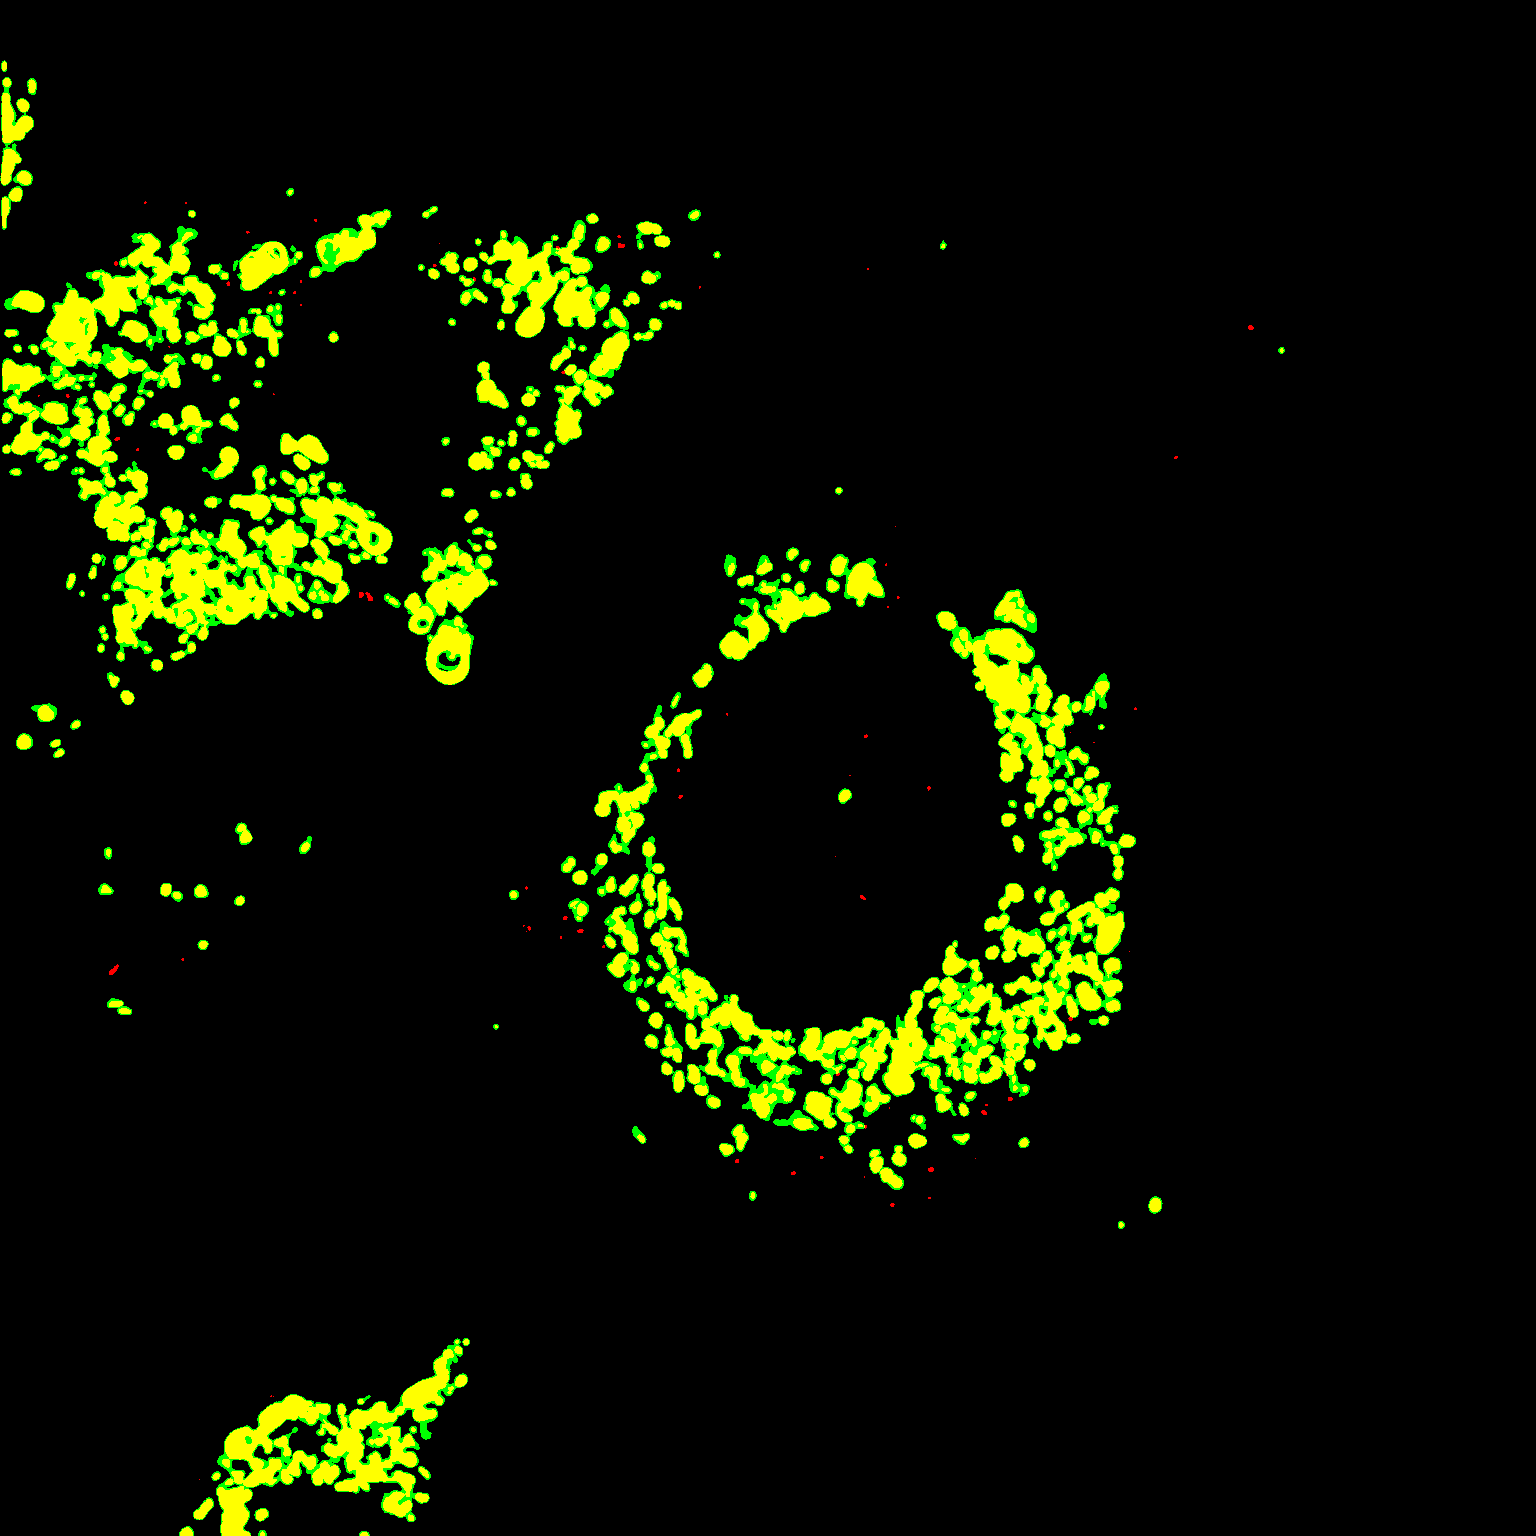
\includegraphics[width=0.32\textwidth]{figs/ch4figs/visual_analysis/global_outcomes/lyso/Moments_LML_4C=0.png}}
	
	\subcaptionbox{Sample A Moments only}{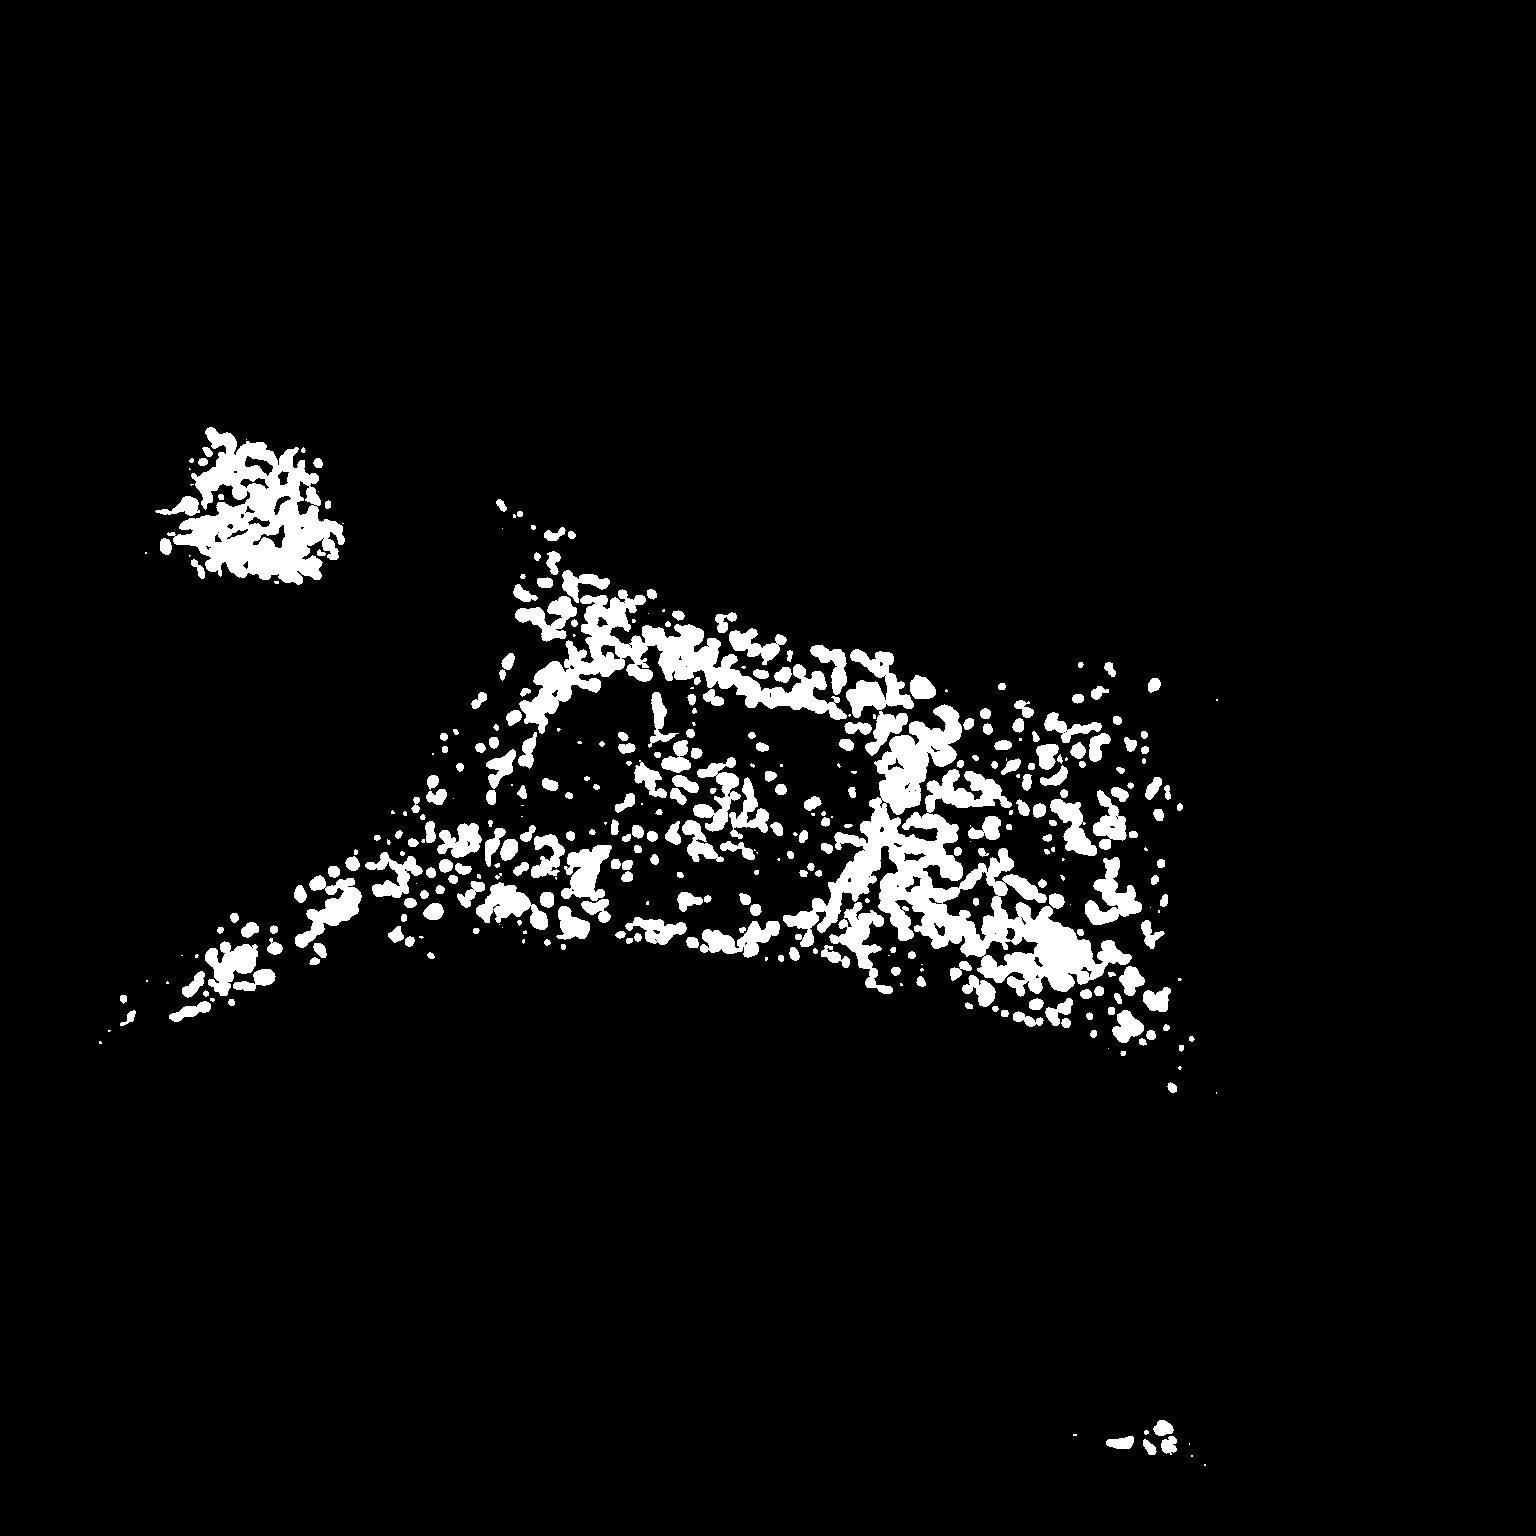
\includegraphics[width=0.32\textwidth]{figs/ch4figs/visual_analysis/global_outcomes/lyso/Flat_Con_2C=0_Moments.png}}
	\subcaptionbox{Sample B Moments only}{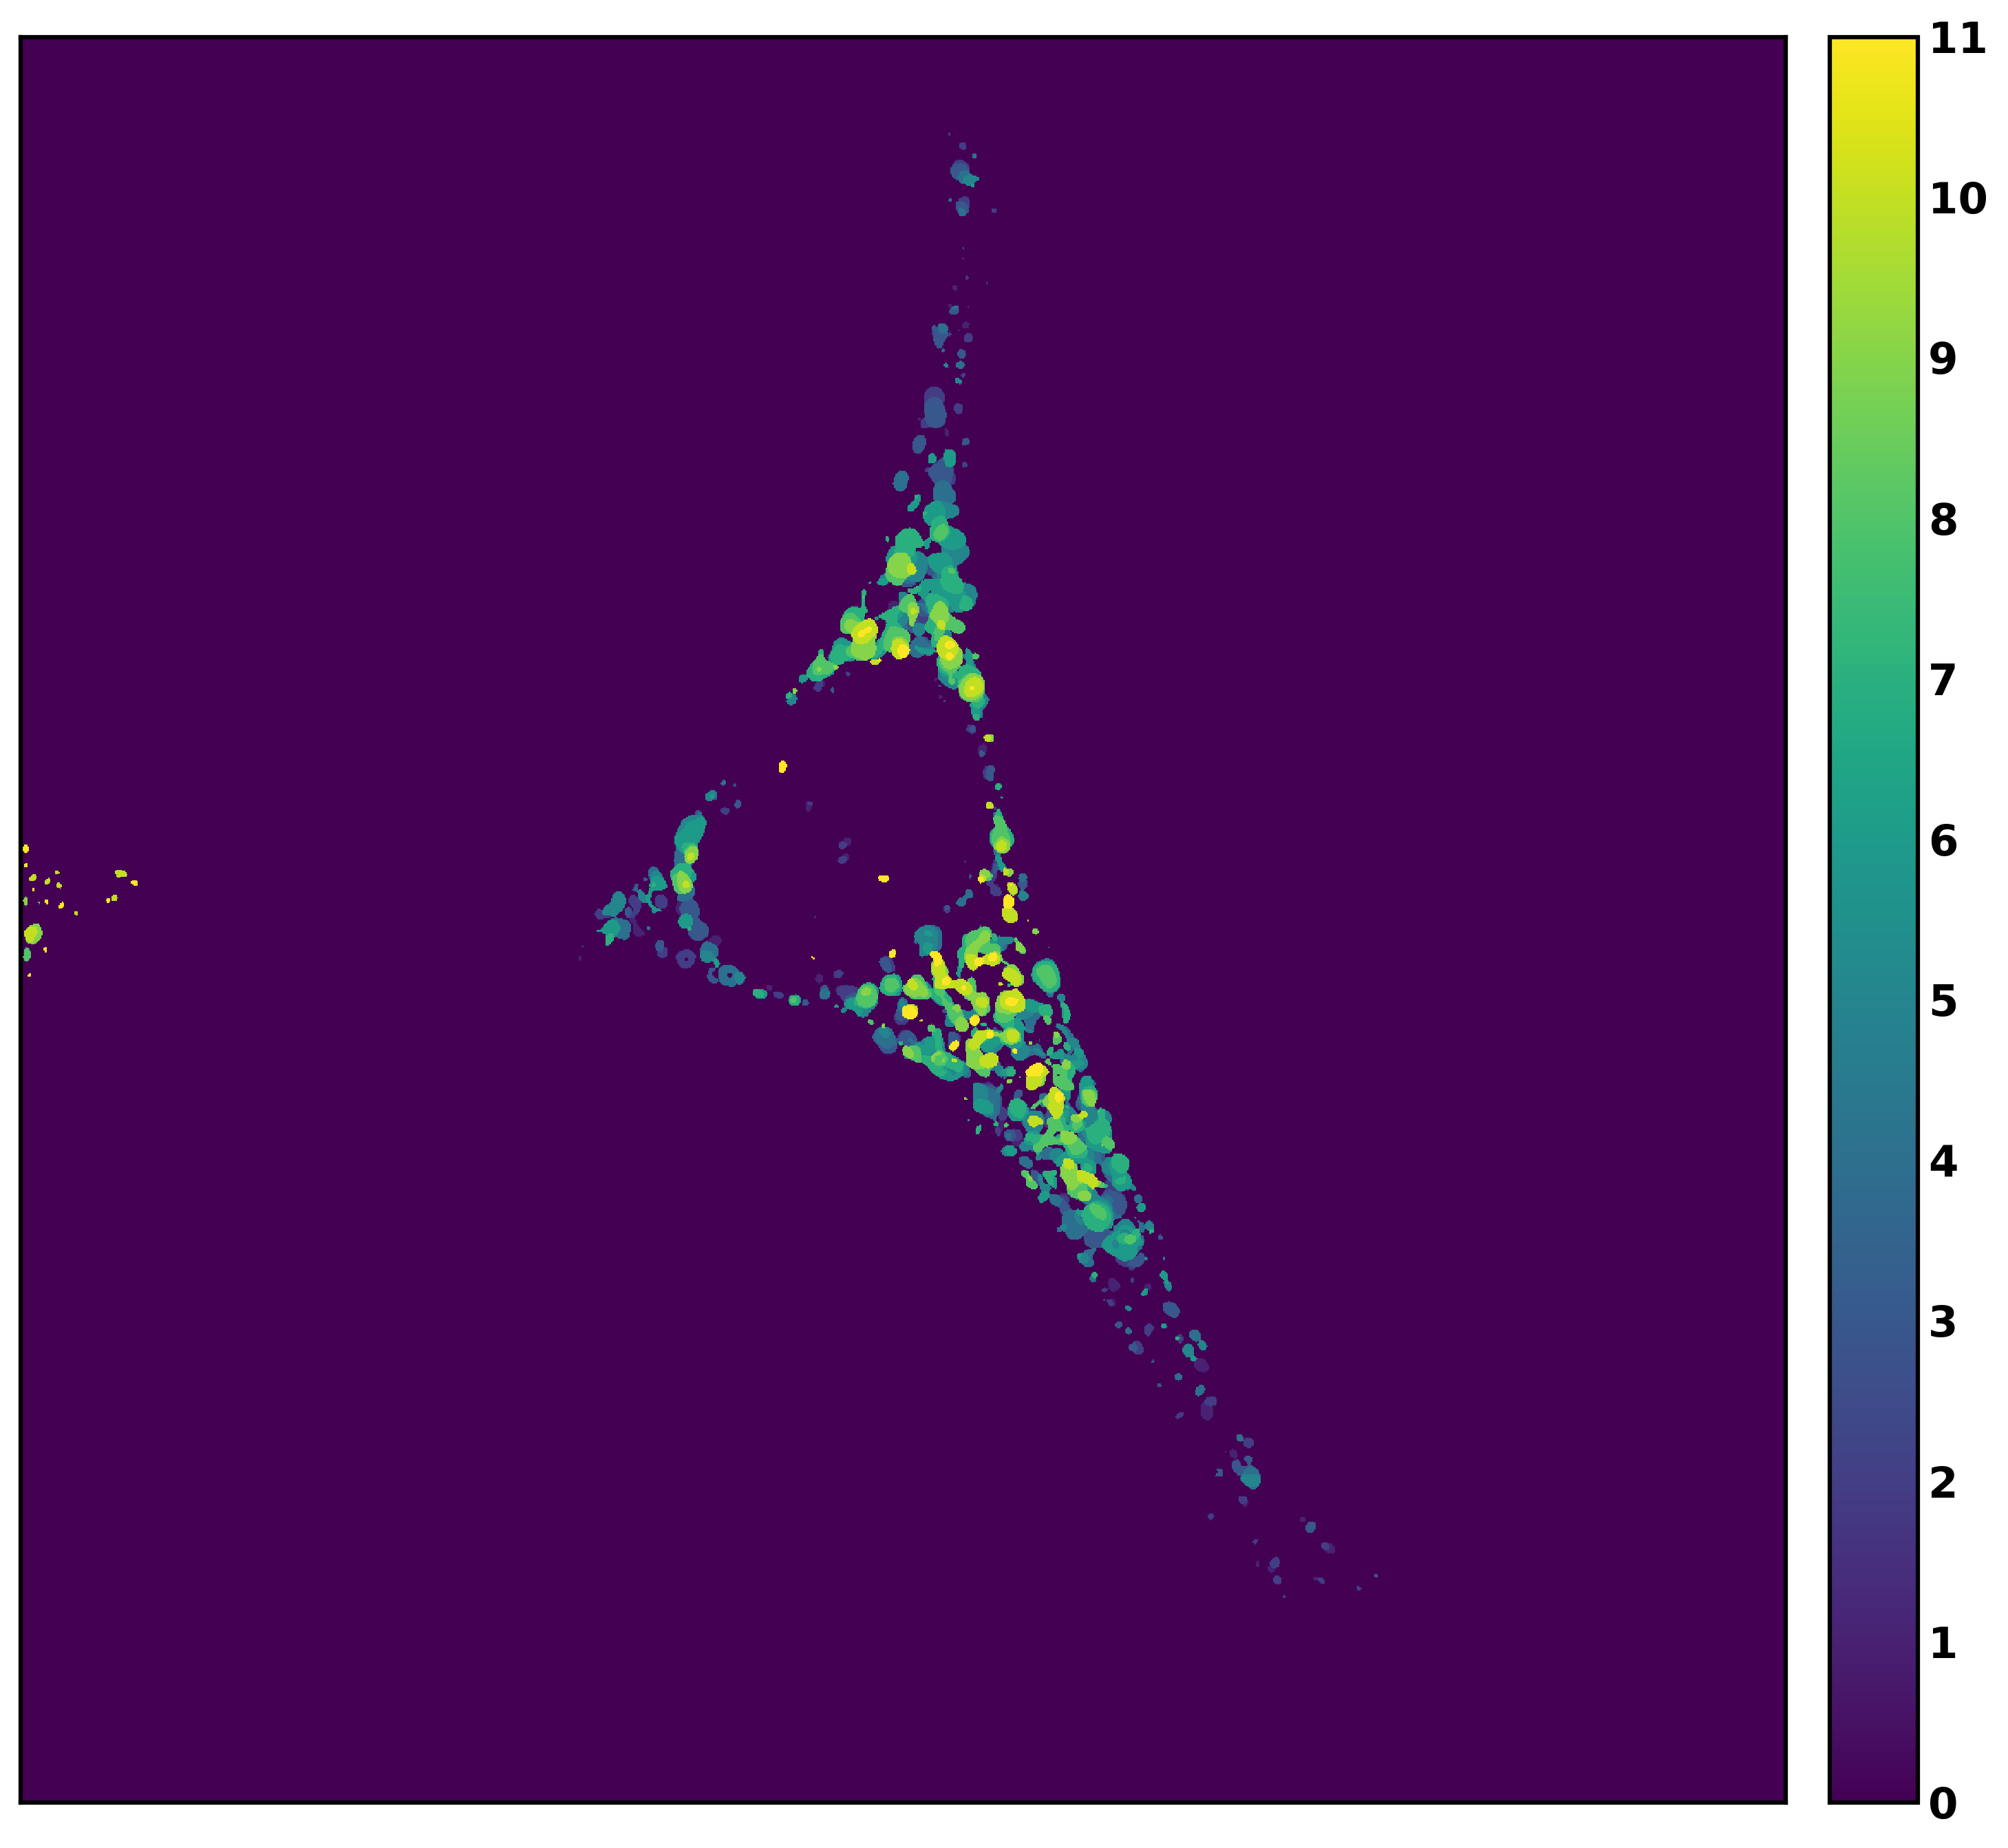
\includegraphics[width=0.32\textwidth]{figs/ch4figs/visual_analysis/global_outcomes/lyso/Flat_LML_3C=0_Moments.png}}
	\subcaptionbox{Sample C Moments only}{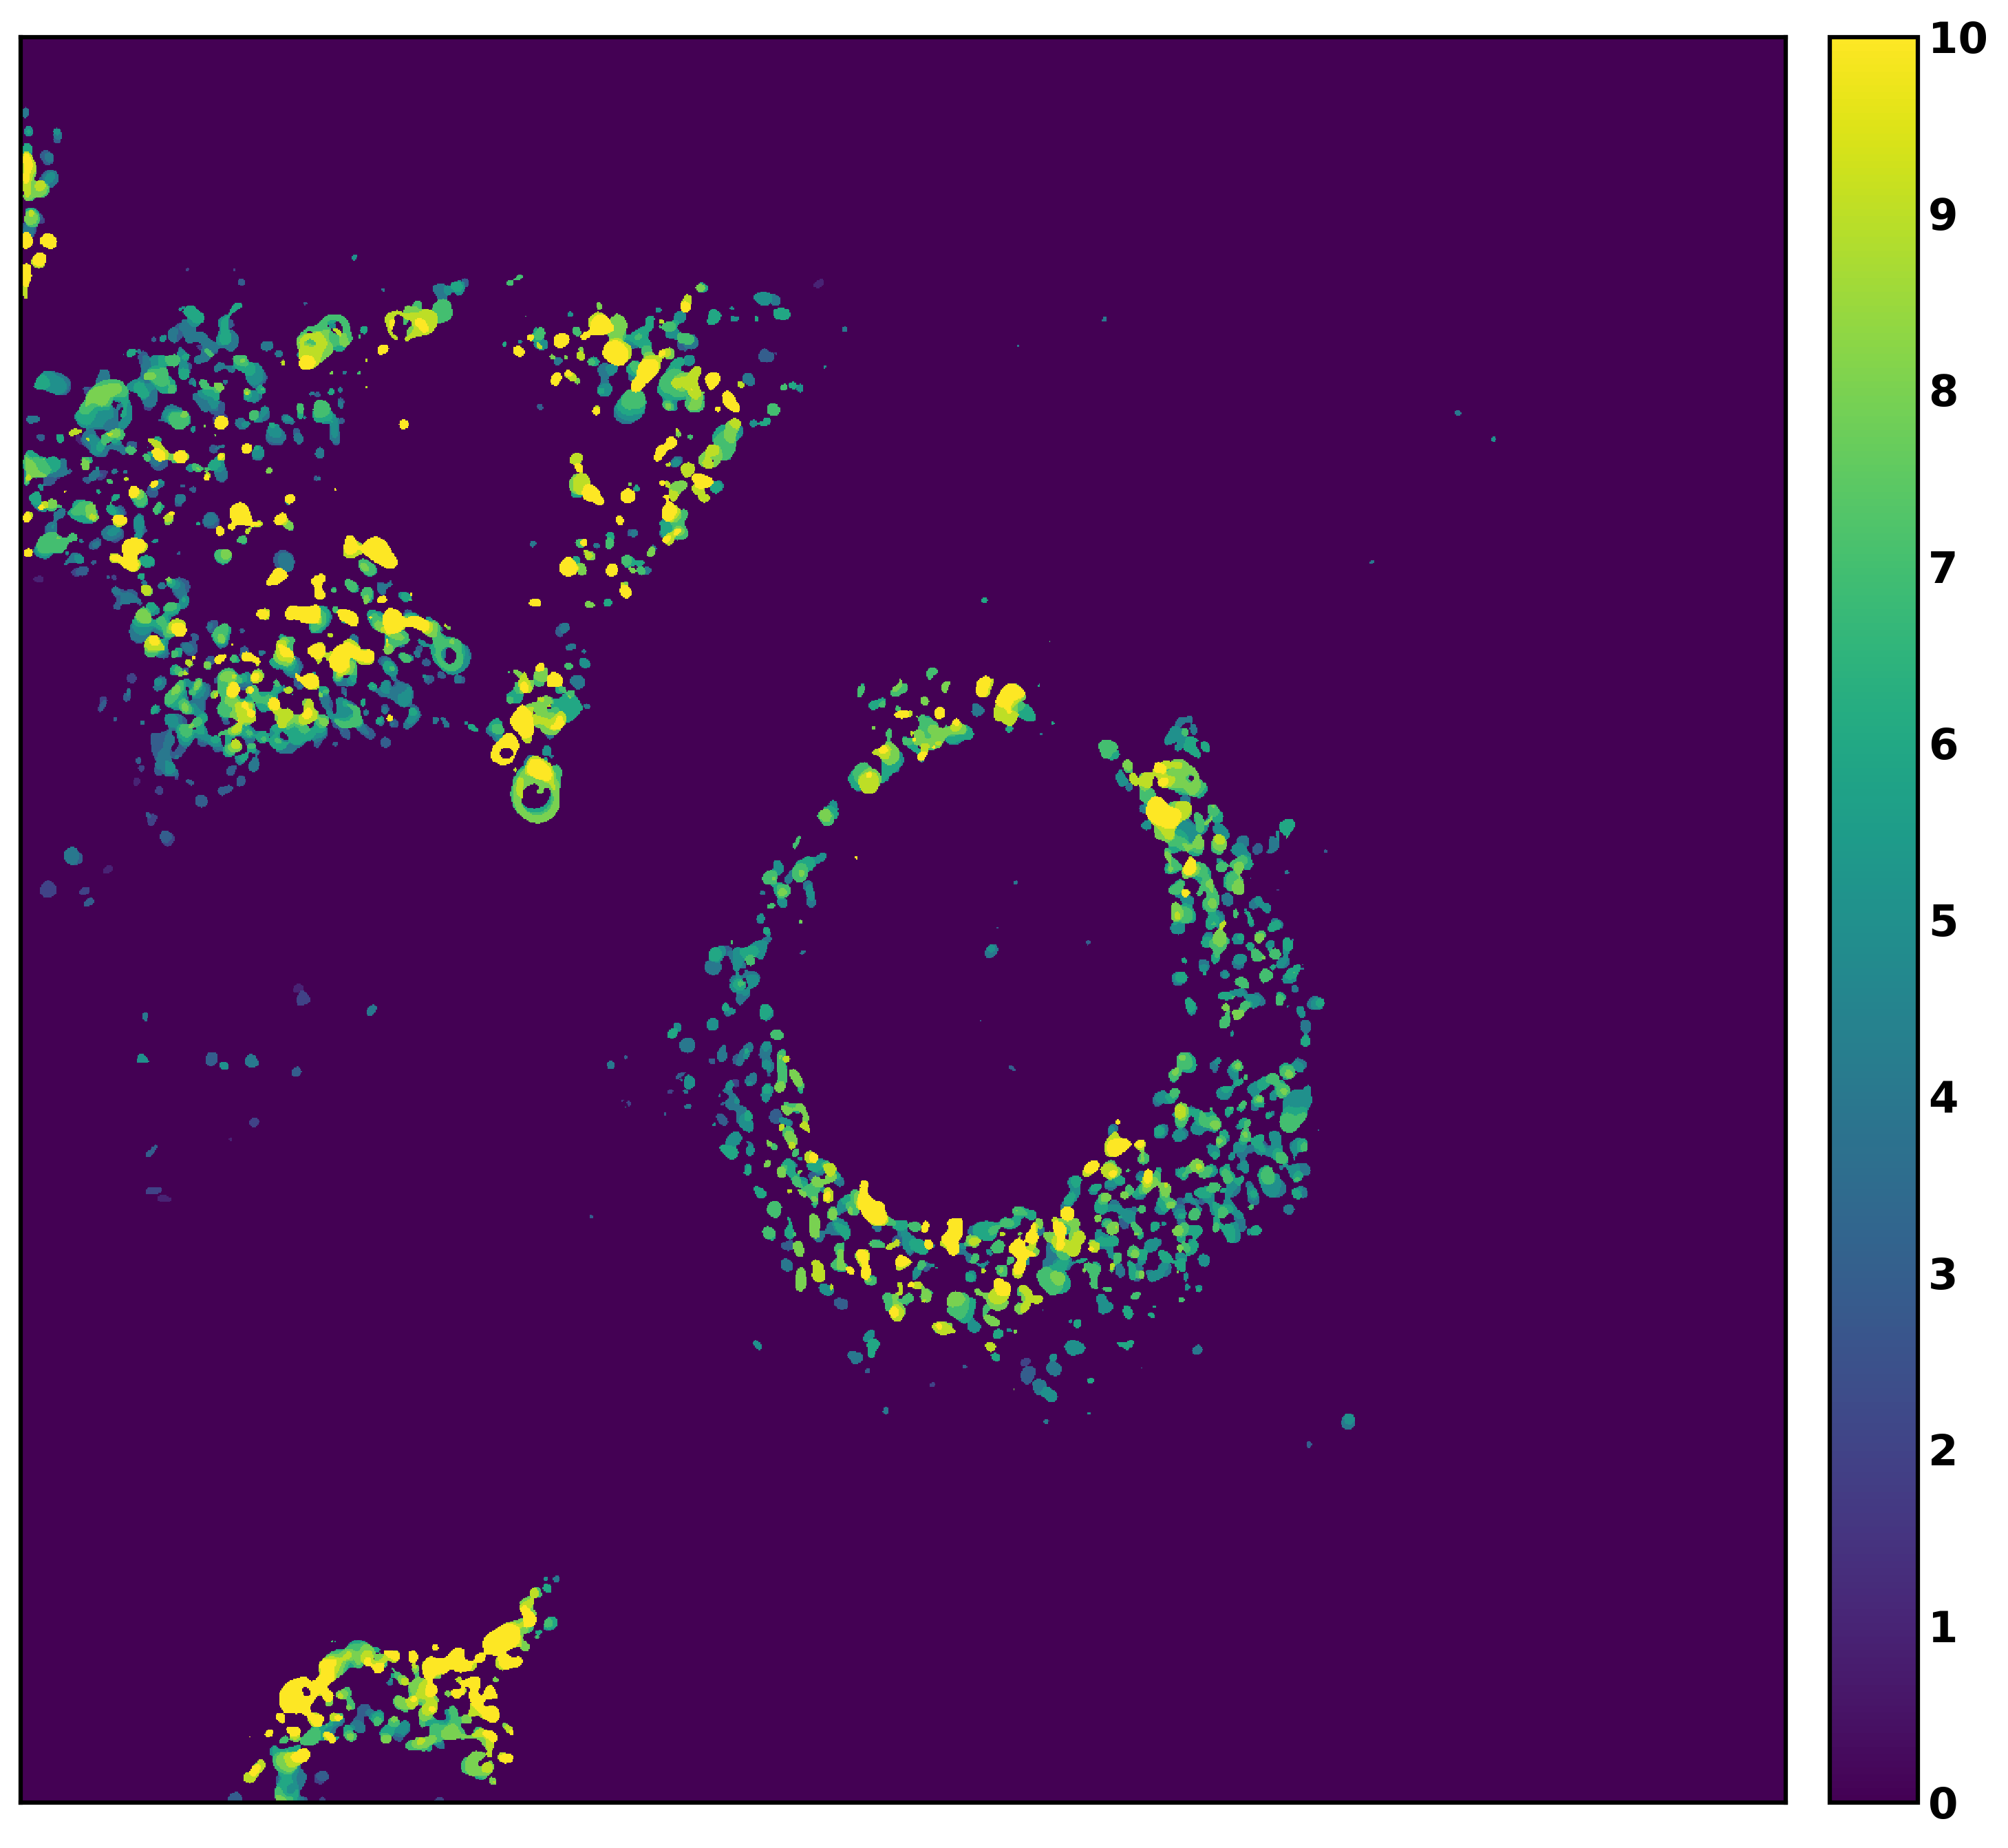
\includegraphics[width=0.32\textwidth]{figs/ch4figs/visual_analysis/global_outcomes/lyso/Flat_LML_4C=0_Moments.png}}
	
	\caption[Showcase of the Moments threshold outcomes with respect to the manual Hysteresis outcomes.]{Showcase of the Moments thresholds outcomes with the top row being red-green overlay images with the Moments outcomes in red, the Hysteresis thresholding outcomes in green, and overlaps of both outcomes in yellow. The bottom row showcases only the Moments thresholding outcomes for improved clarity.}
	\label{fig:lyso_moments}
\end{figure}

\FloatBarrier
\paragraph{IsoData} The showcase of the IsoData threshold outcomes is shown in Figure \ref{fig:lyso_isodata} with the IsoData threshold outcomes compared against the Hysteresis threshold outcomes in a red-green image for each sample. There are also binarized images for each sample of only the IsoData threshold outcomes which matches the red colour channel in the red-green images. The IsoData outcomes for all of the lysosome samples are quite similar to the Hysteresis thresholding outcomes although each expresses a minor degree of under-thresholding. This is observed to be a highly effective lysosome structure thresholding method as the extra structures captured by IsoData, that are not present in the Hysteresis threshold outcomes, are for structures with a mean intensity closer to the Hysteresis thresholding labelled foreground structures than the background.

\begin{figure}[h!]
	\subcaptionbox{Sample A overlayed}{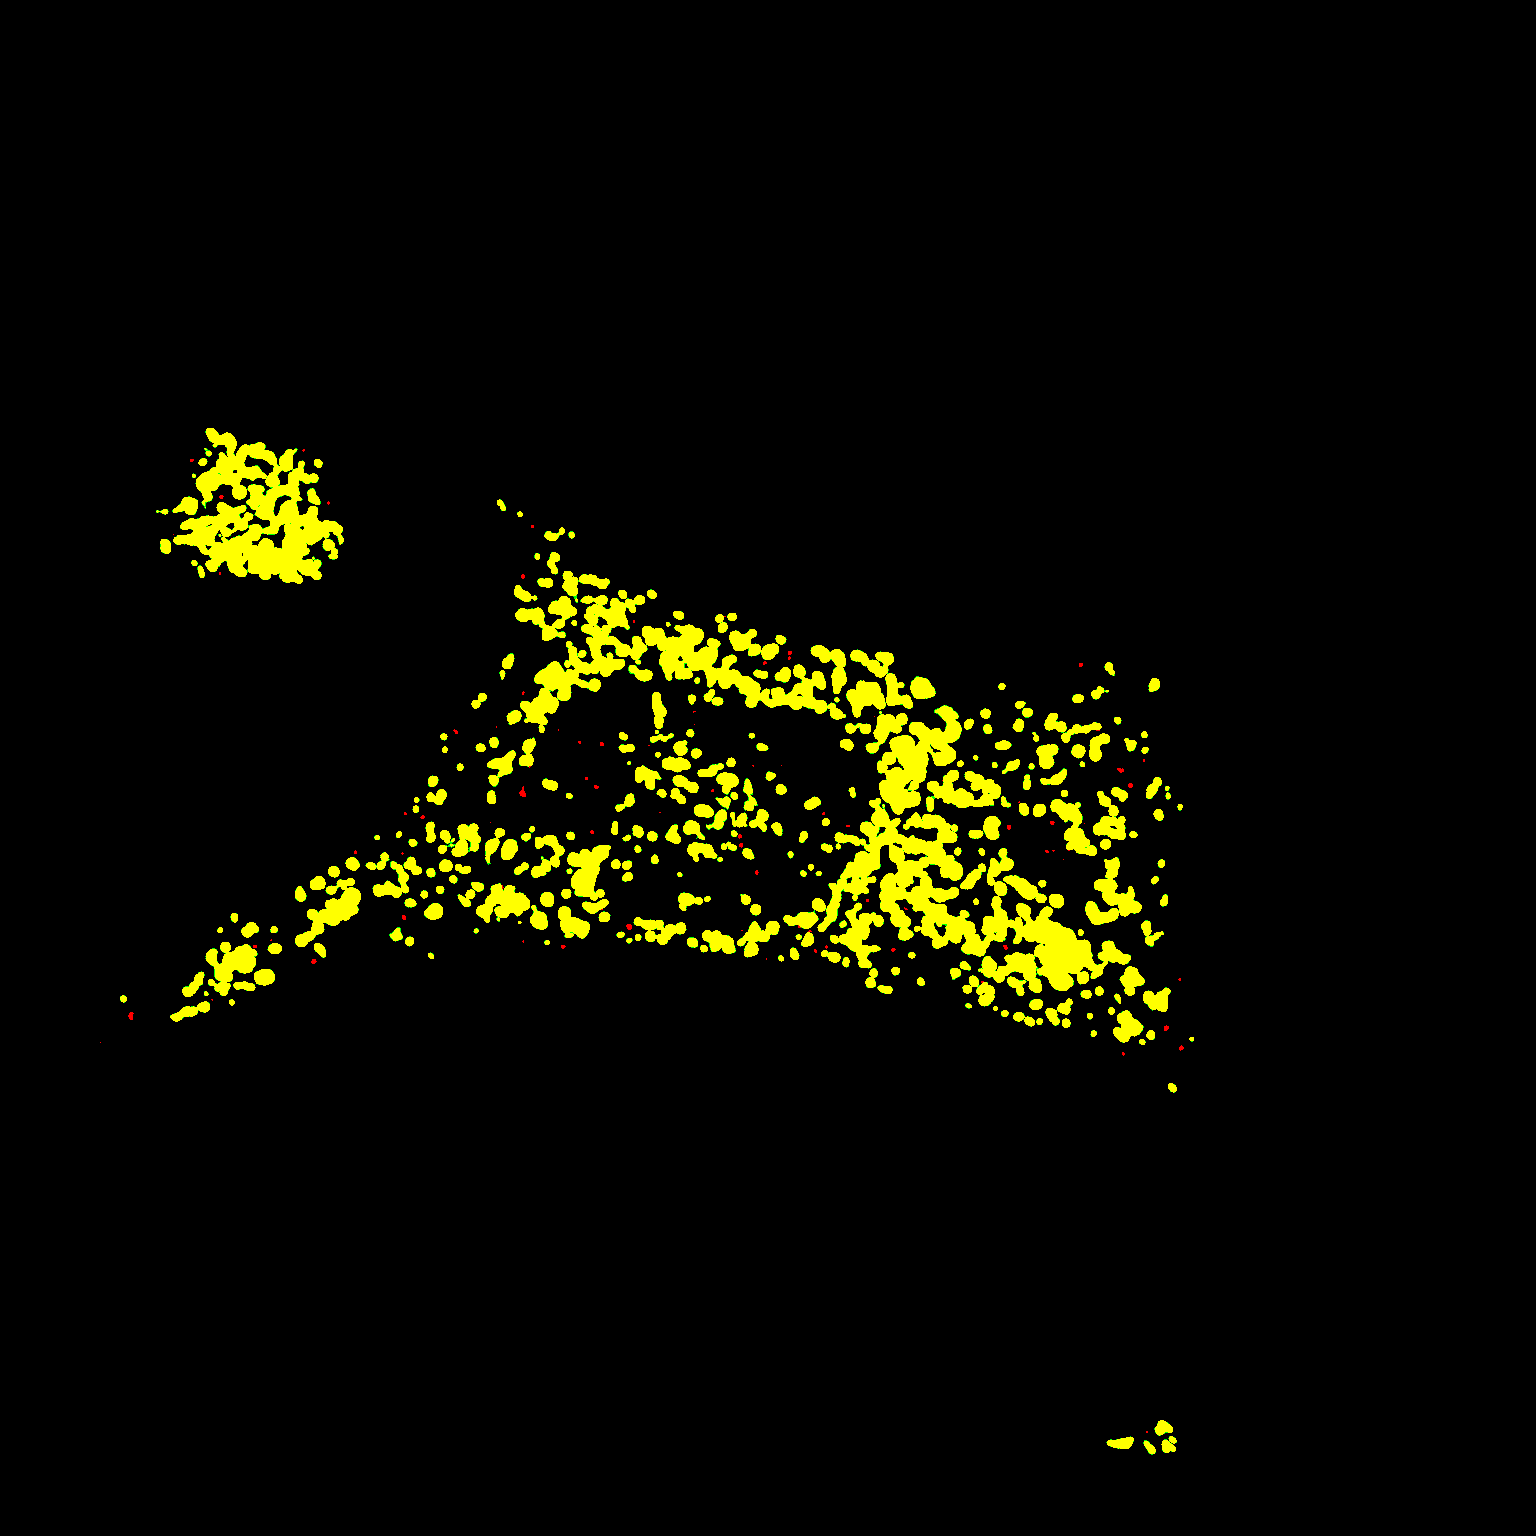
\includegraphics[width=0.32\textwidth]{figs/ch4figs/visual_analysis/global_outcomes/lyso/IsoData_Con_2C=0.png}}
	\subcaptionbox{Sample B overlayed}{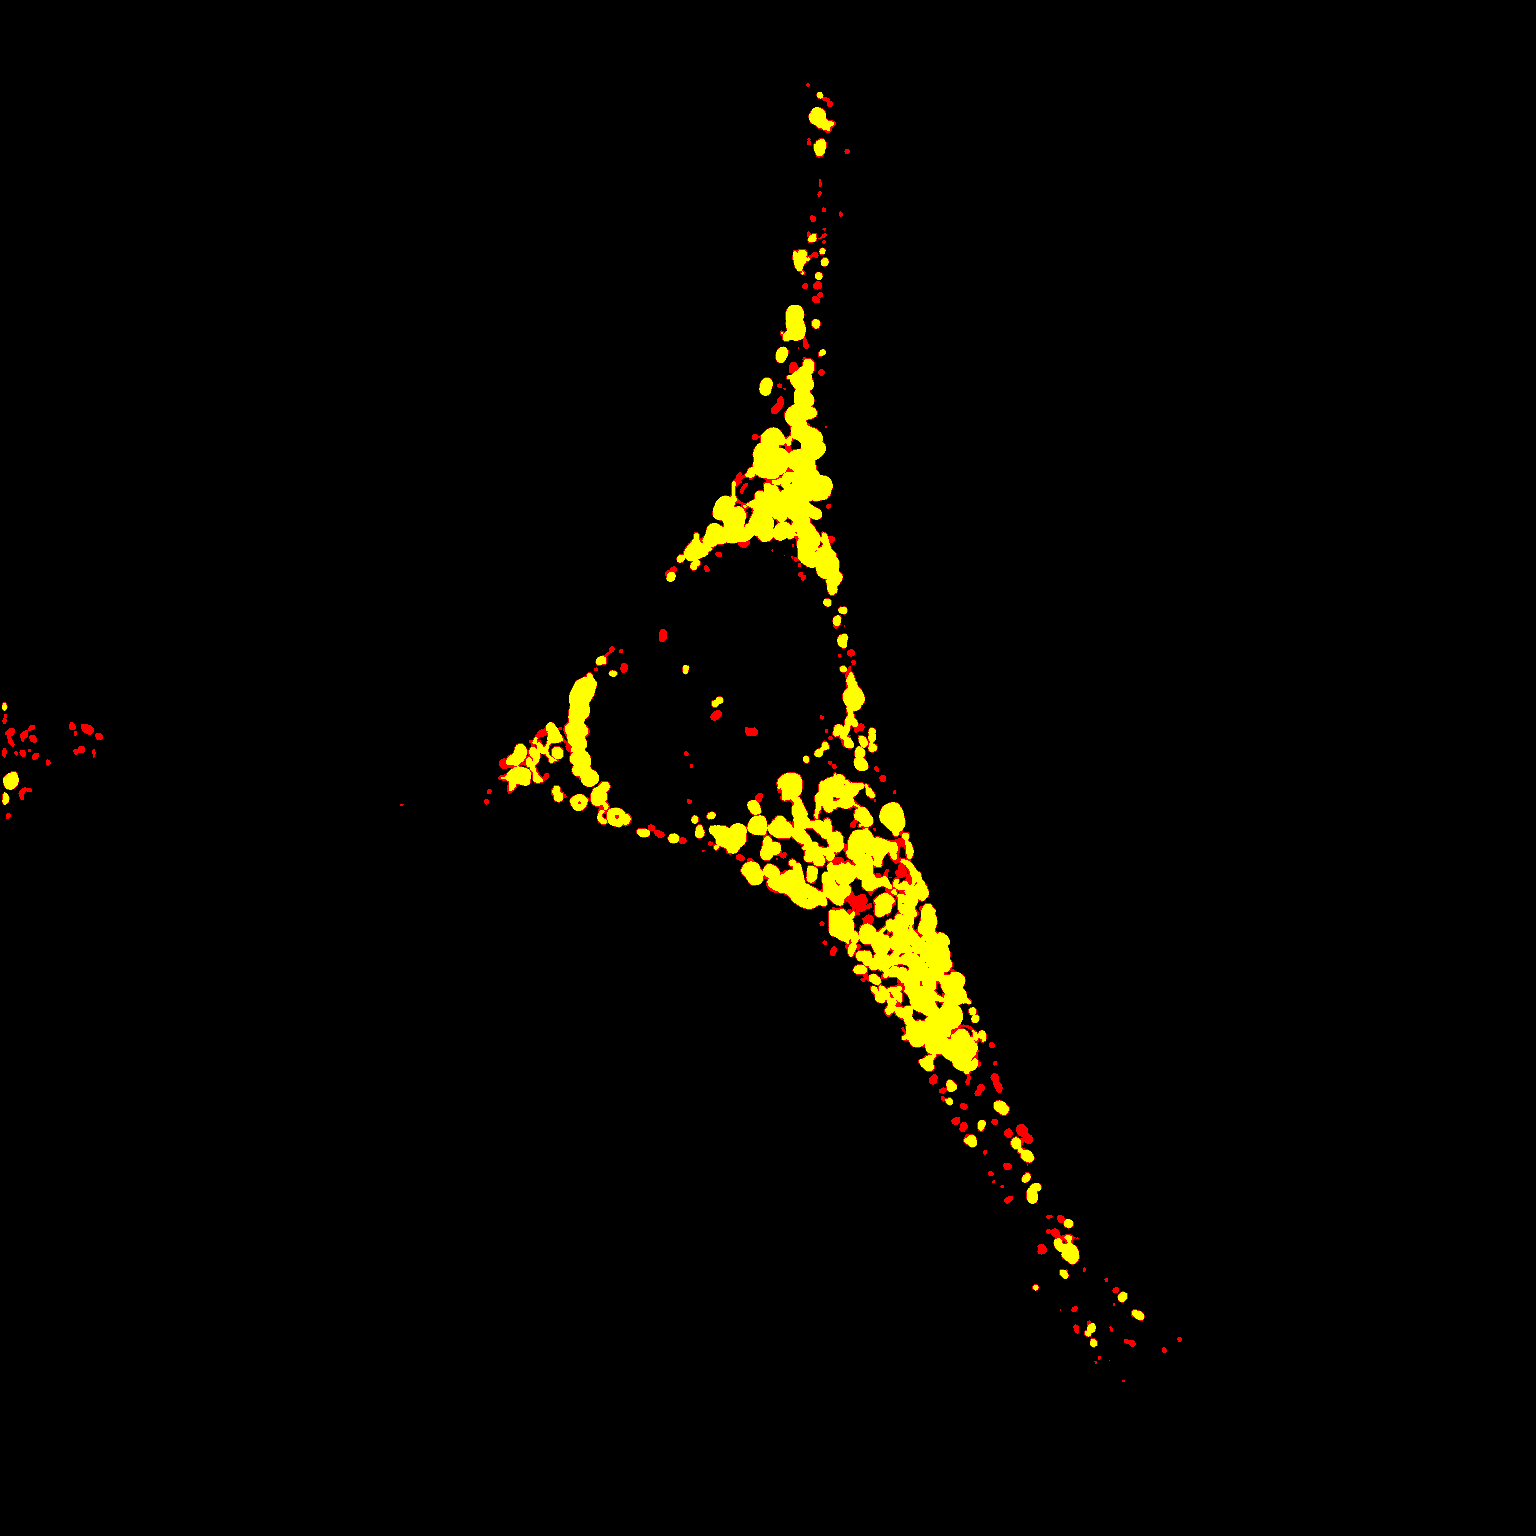
\includegraphics[width=0.32\textwidth]{figs/ch4figs/visual_analysis/global_outcomes/lyso/IsoData_LML_3C=0.png}}
	\subcaptionbox{Sample C overlayed}{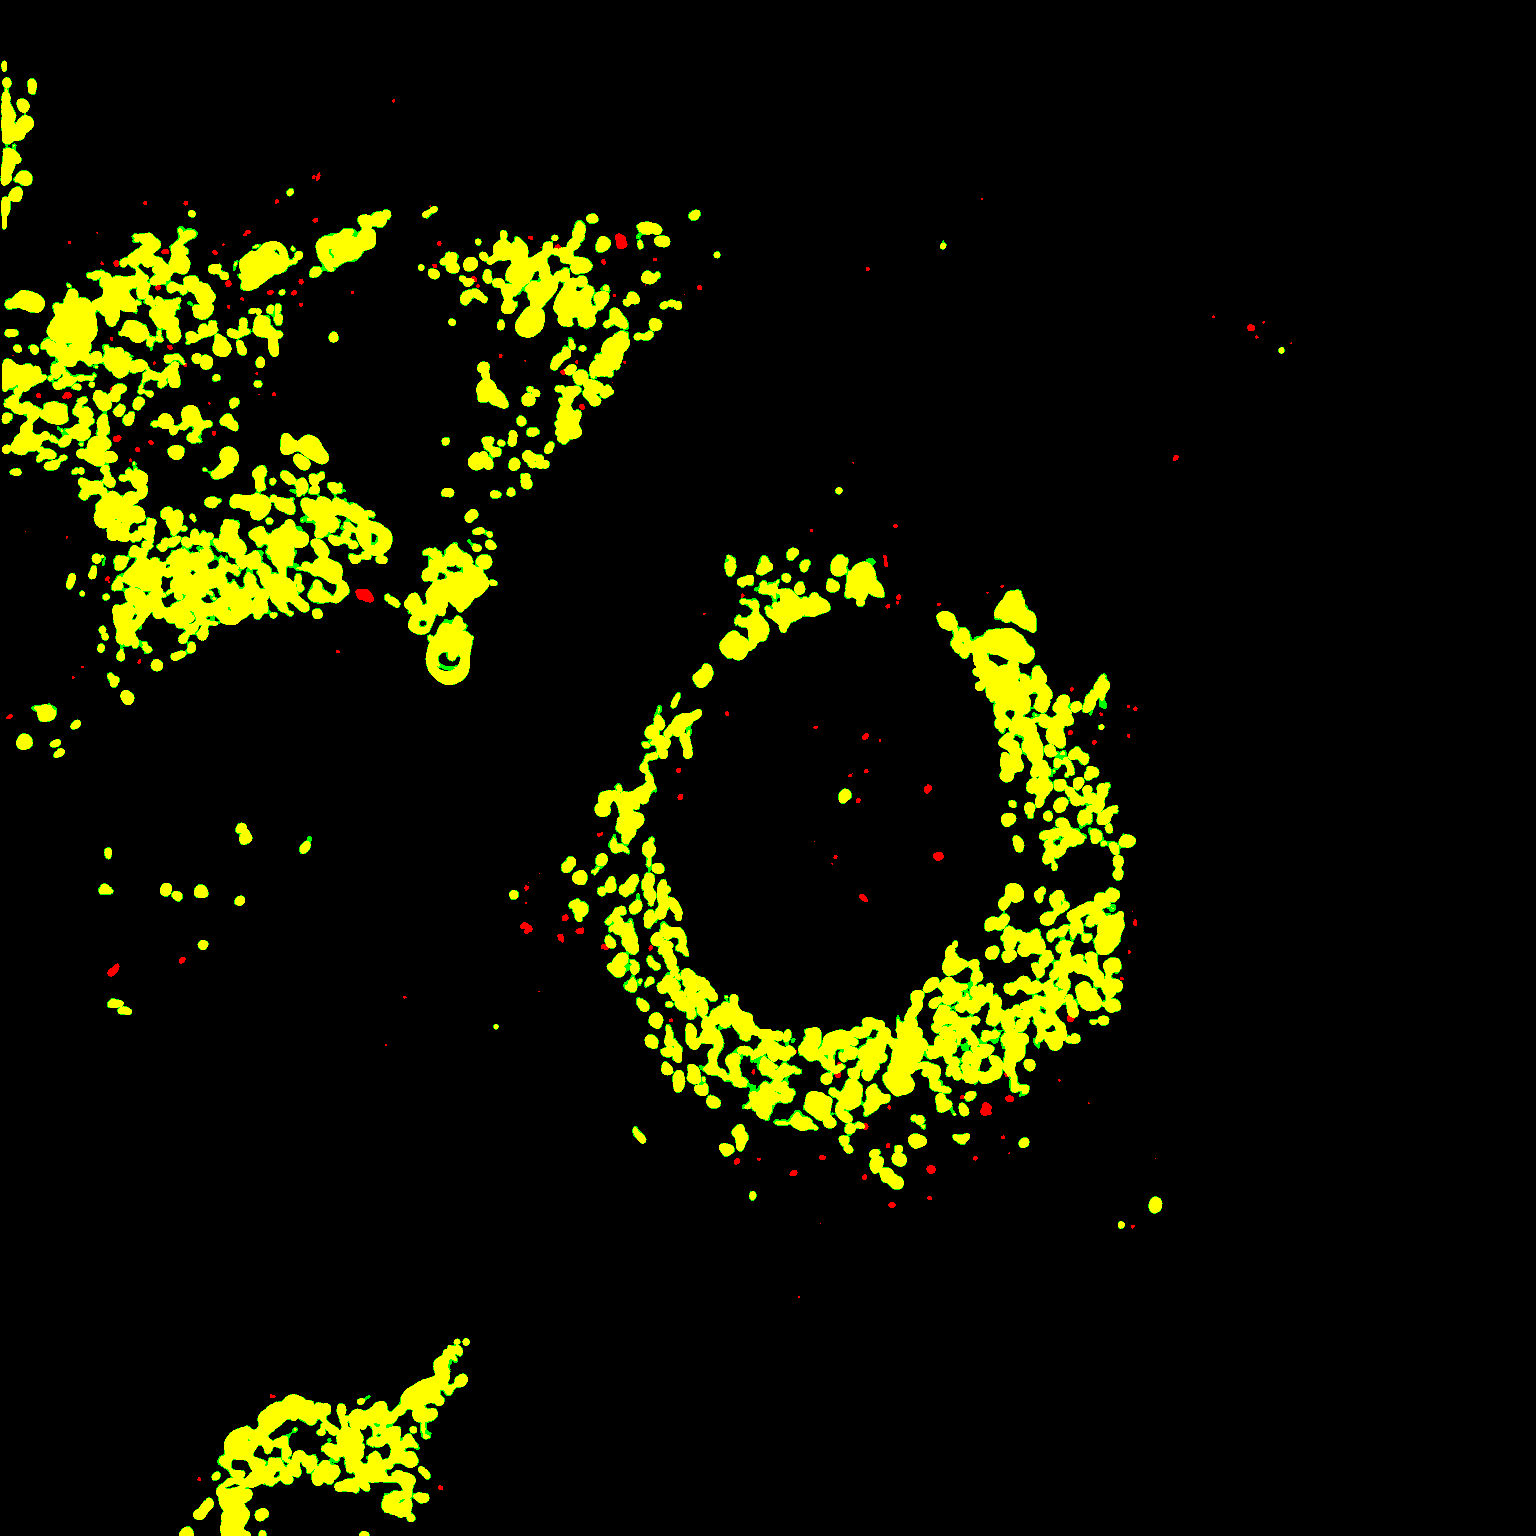
\includegraphics[width=0.32\textwidth]{figs/ch4figs/visual_analysis/global_outcomes/lyso/IsoData_LML_4C=0.png}}
	
	\subcaptionbox{Sample A IsoData only}{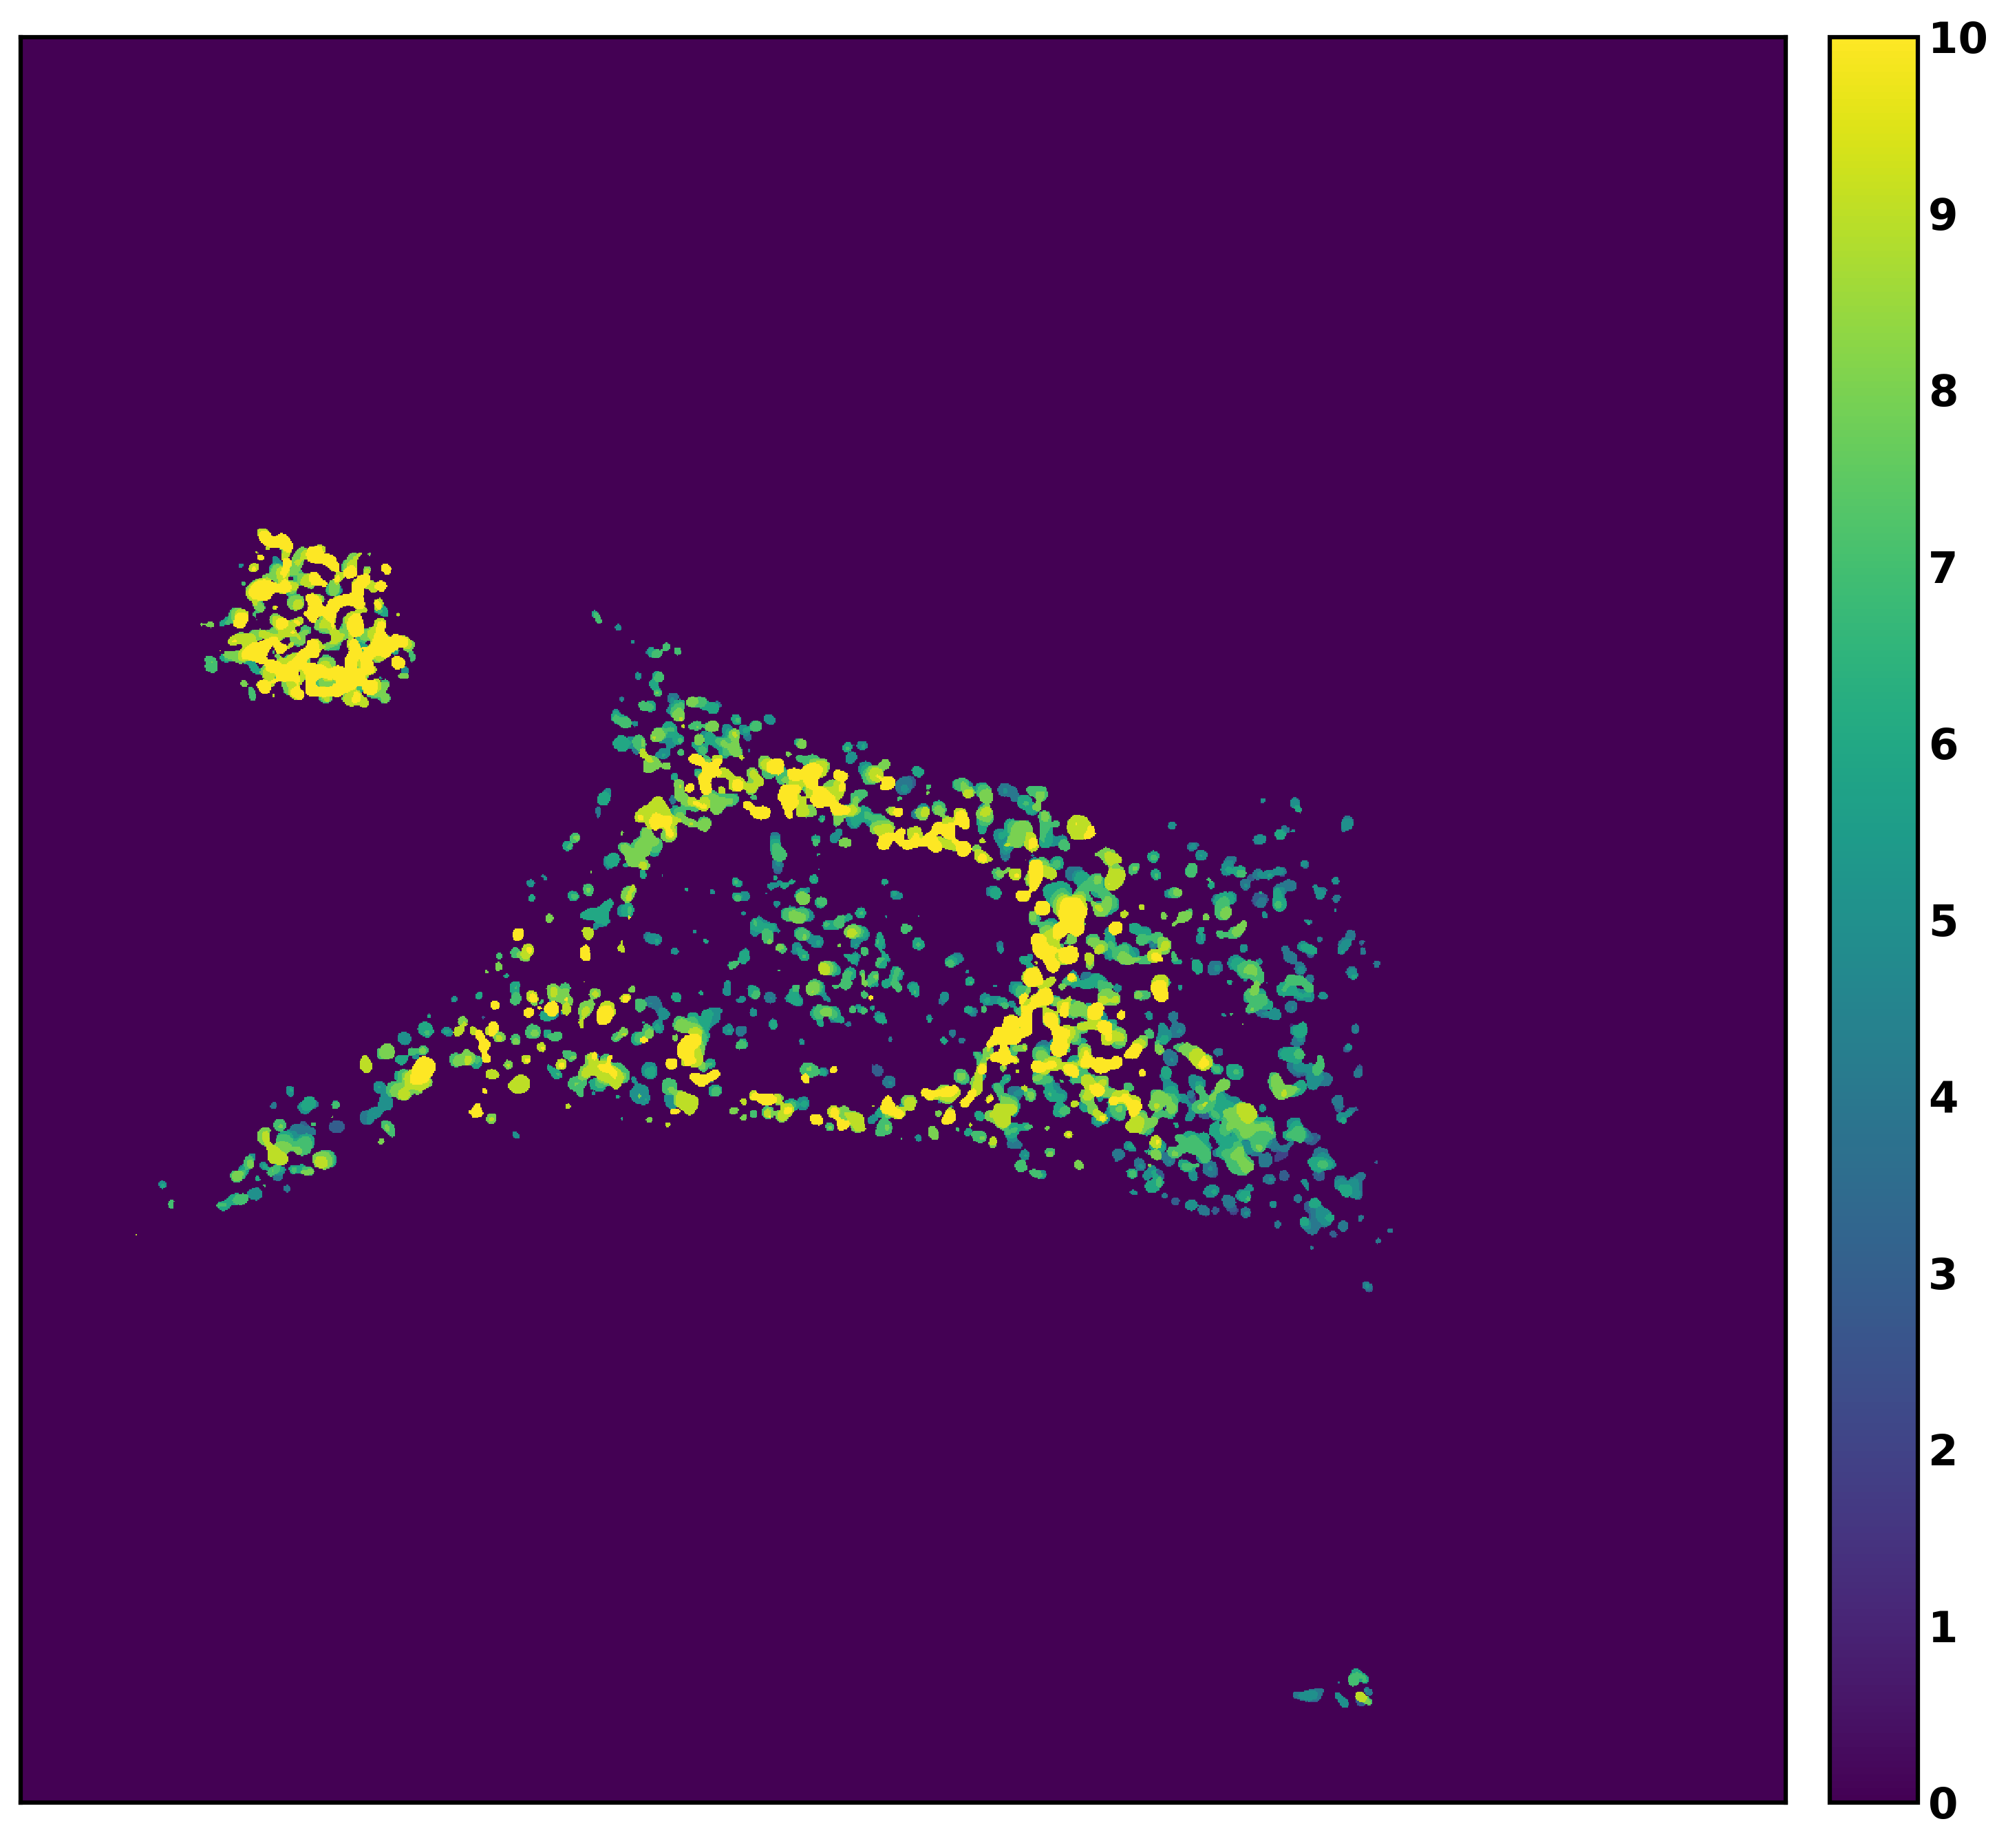
\includegraphics[width=0.32\textwidth]{figs/ch4figs/visual_analysis/global_outcomes/lyso/Flat_Con_2C=0_IsoData.png}}
	\subcaptionbox{Sample B IsoData only}{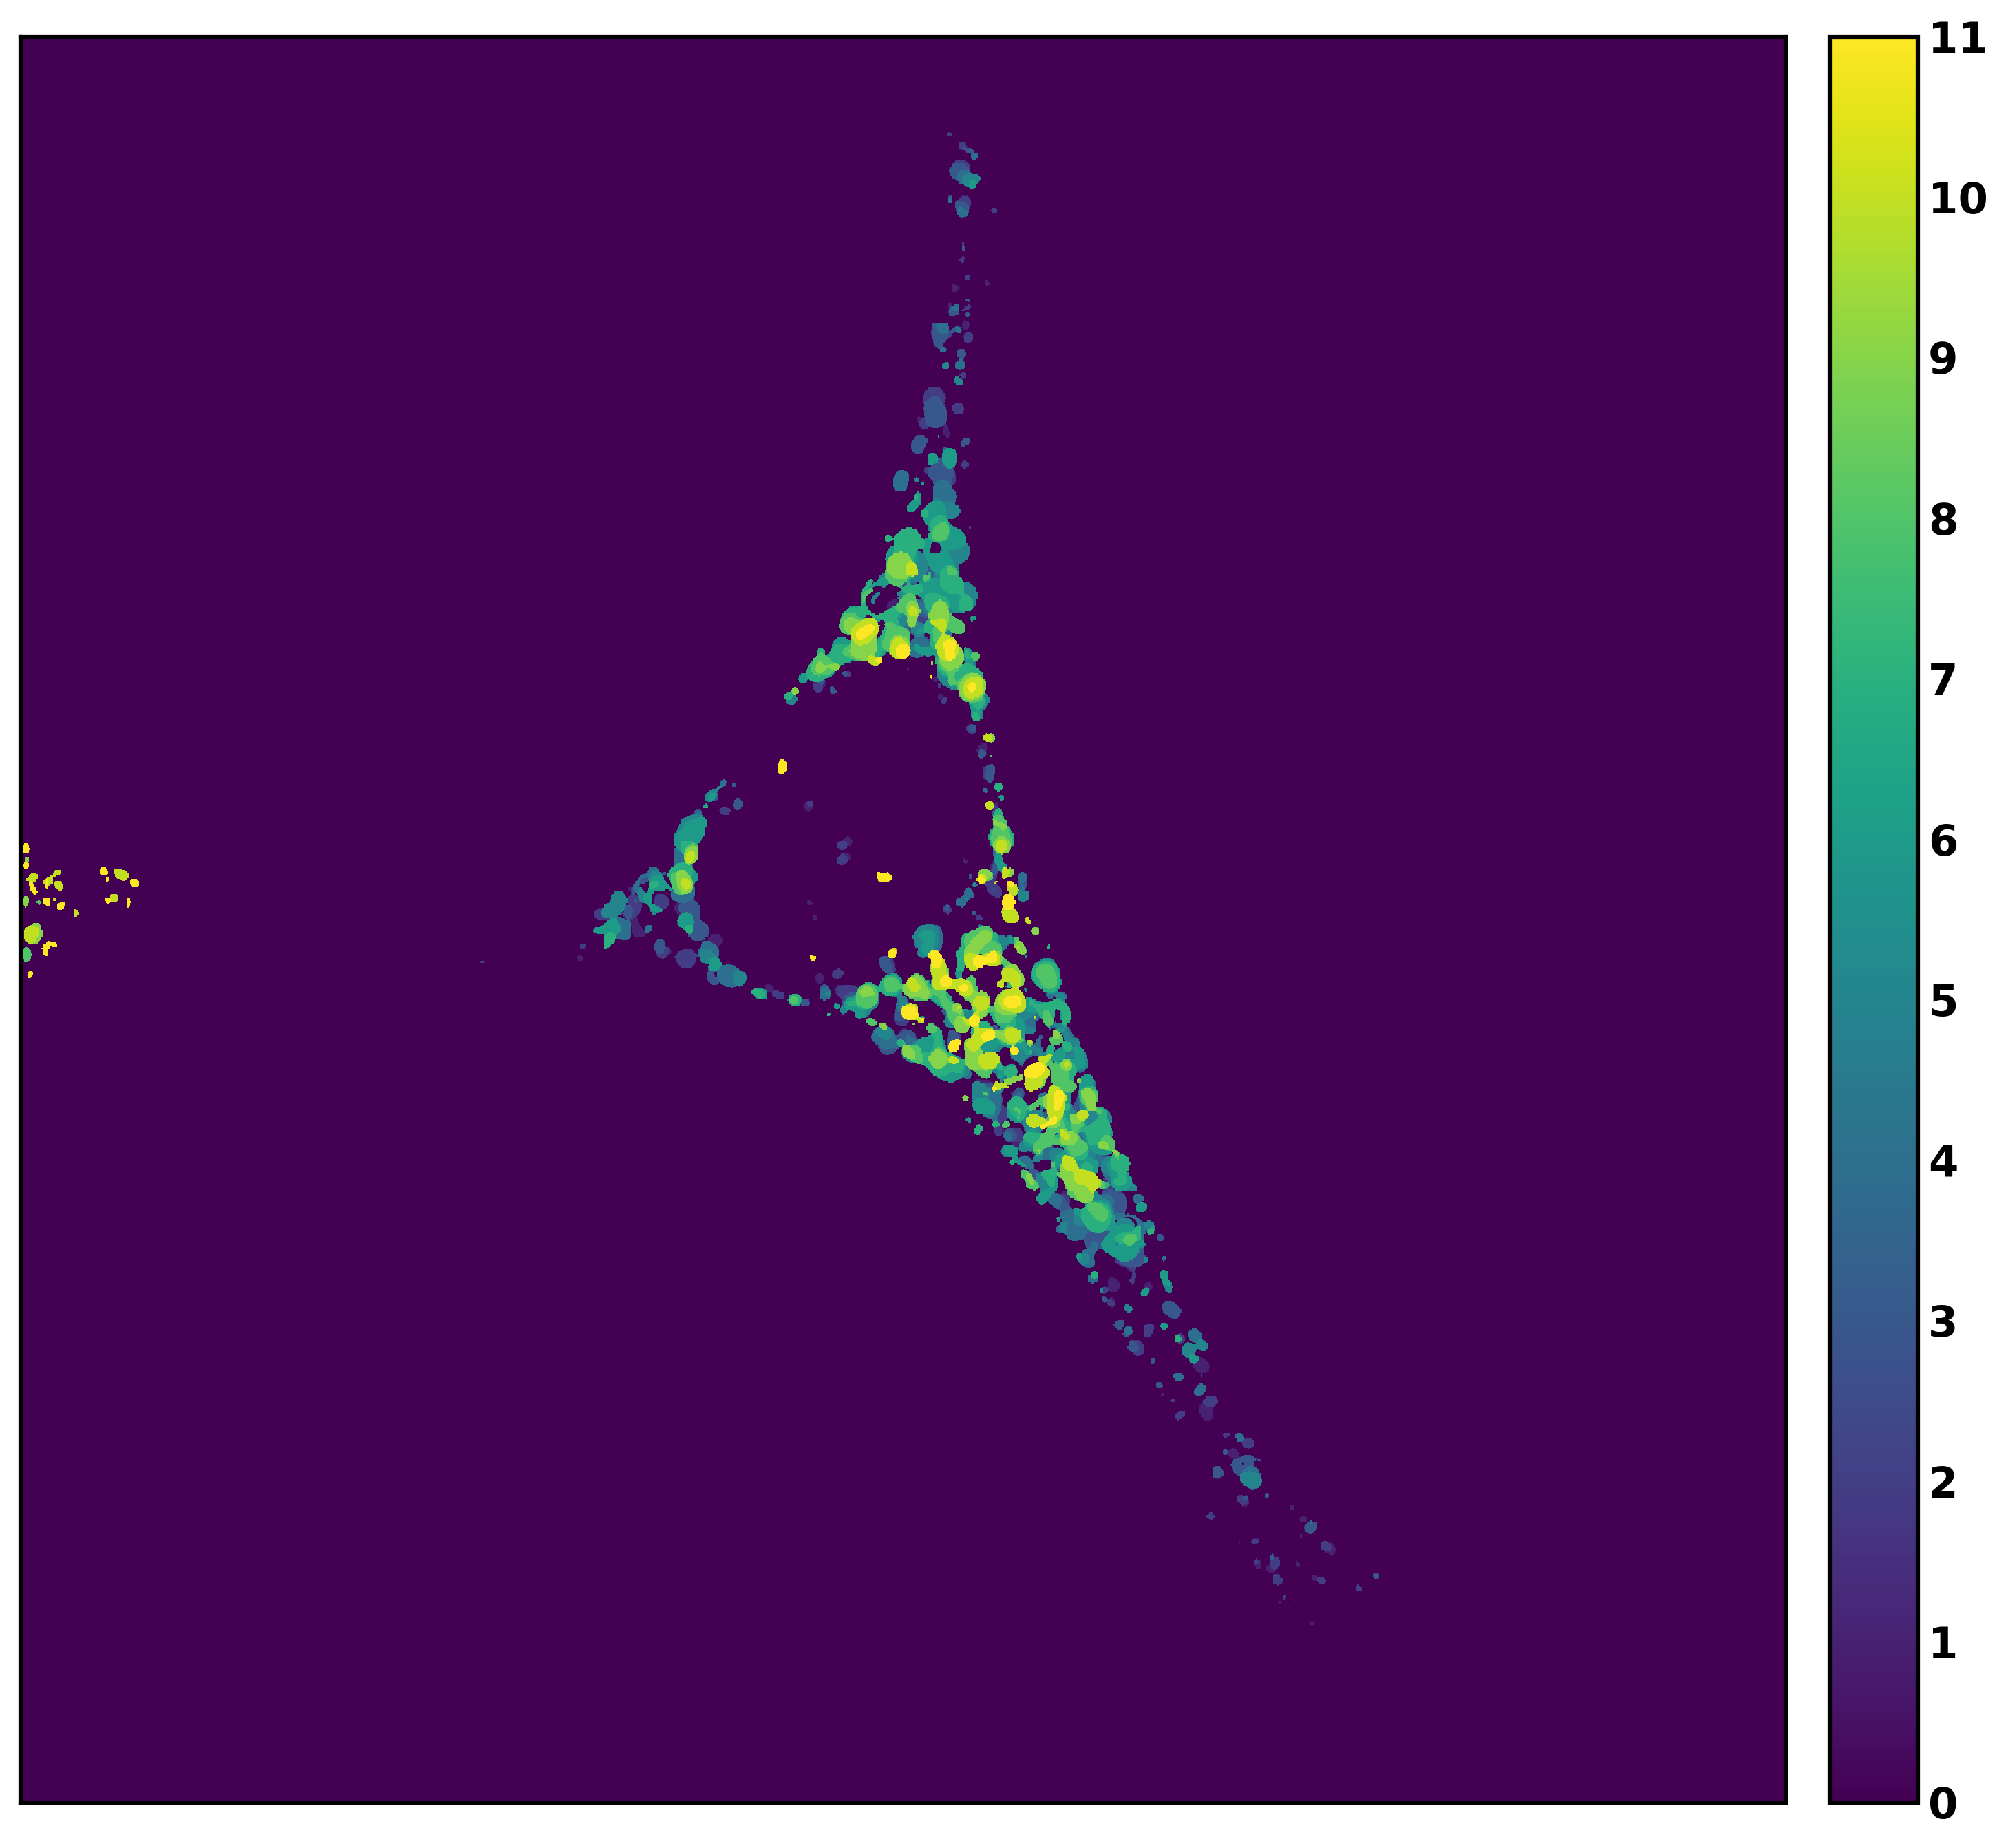
\includegraphics[width=0.32\textwidth]{figs/ch4figs/visual_analysis/global_outcomes/lyso/Flat_LML_3C=0_IsoData.png}}
	\subcaptionbox{Sample C IsoData only}{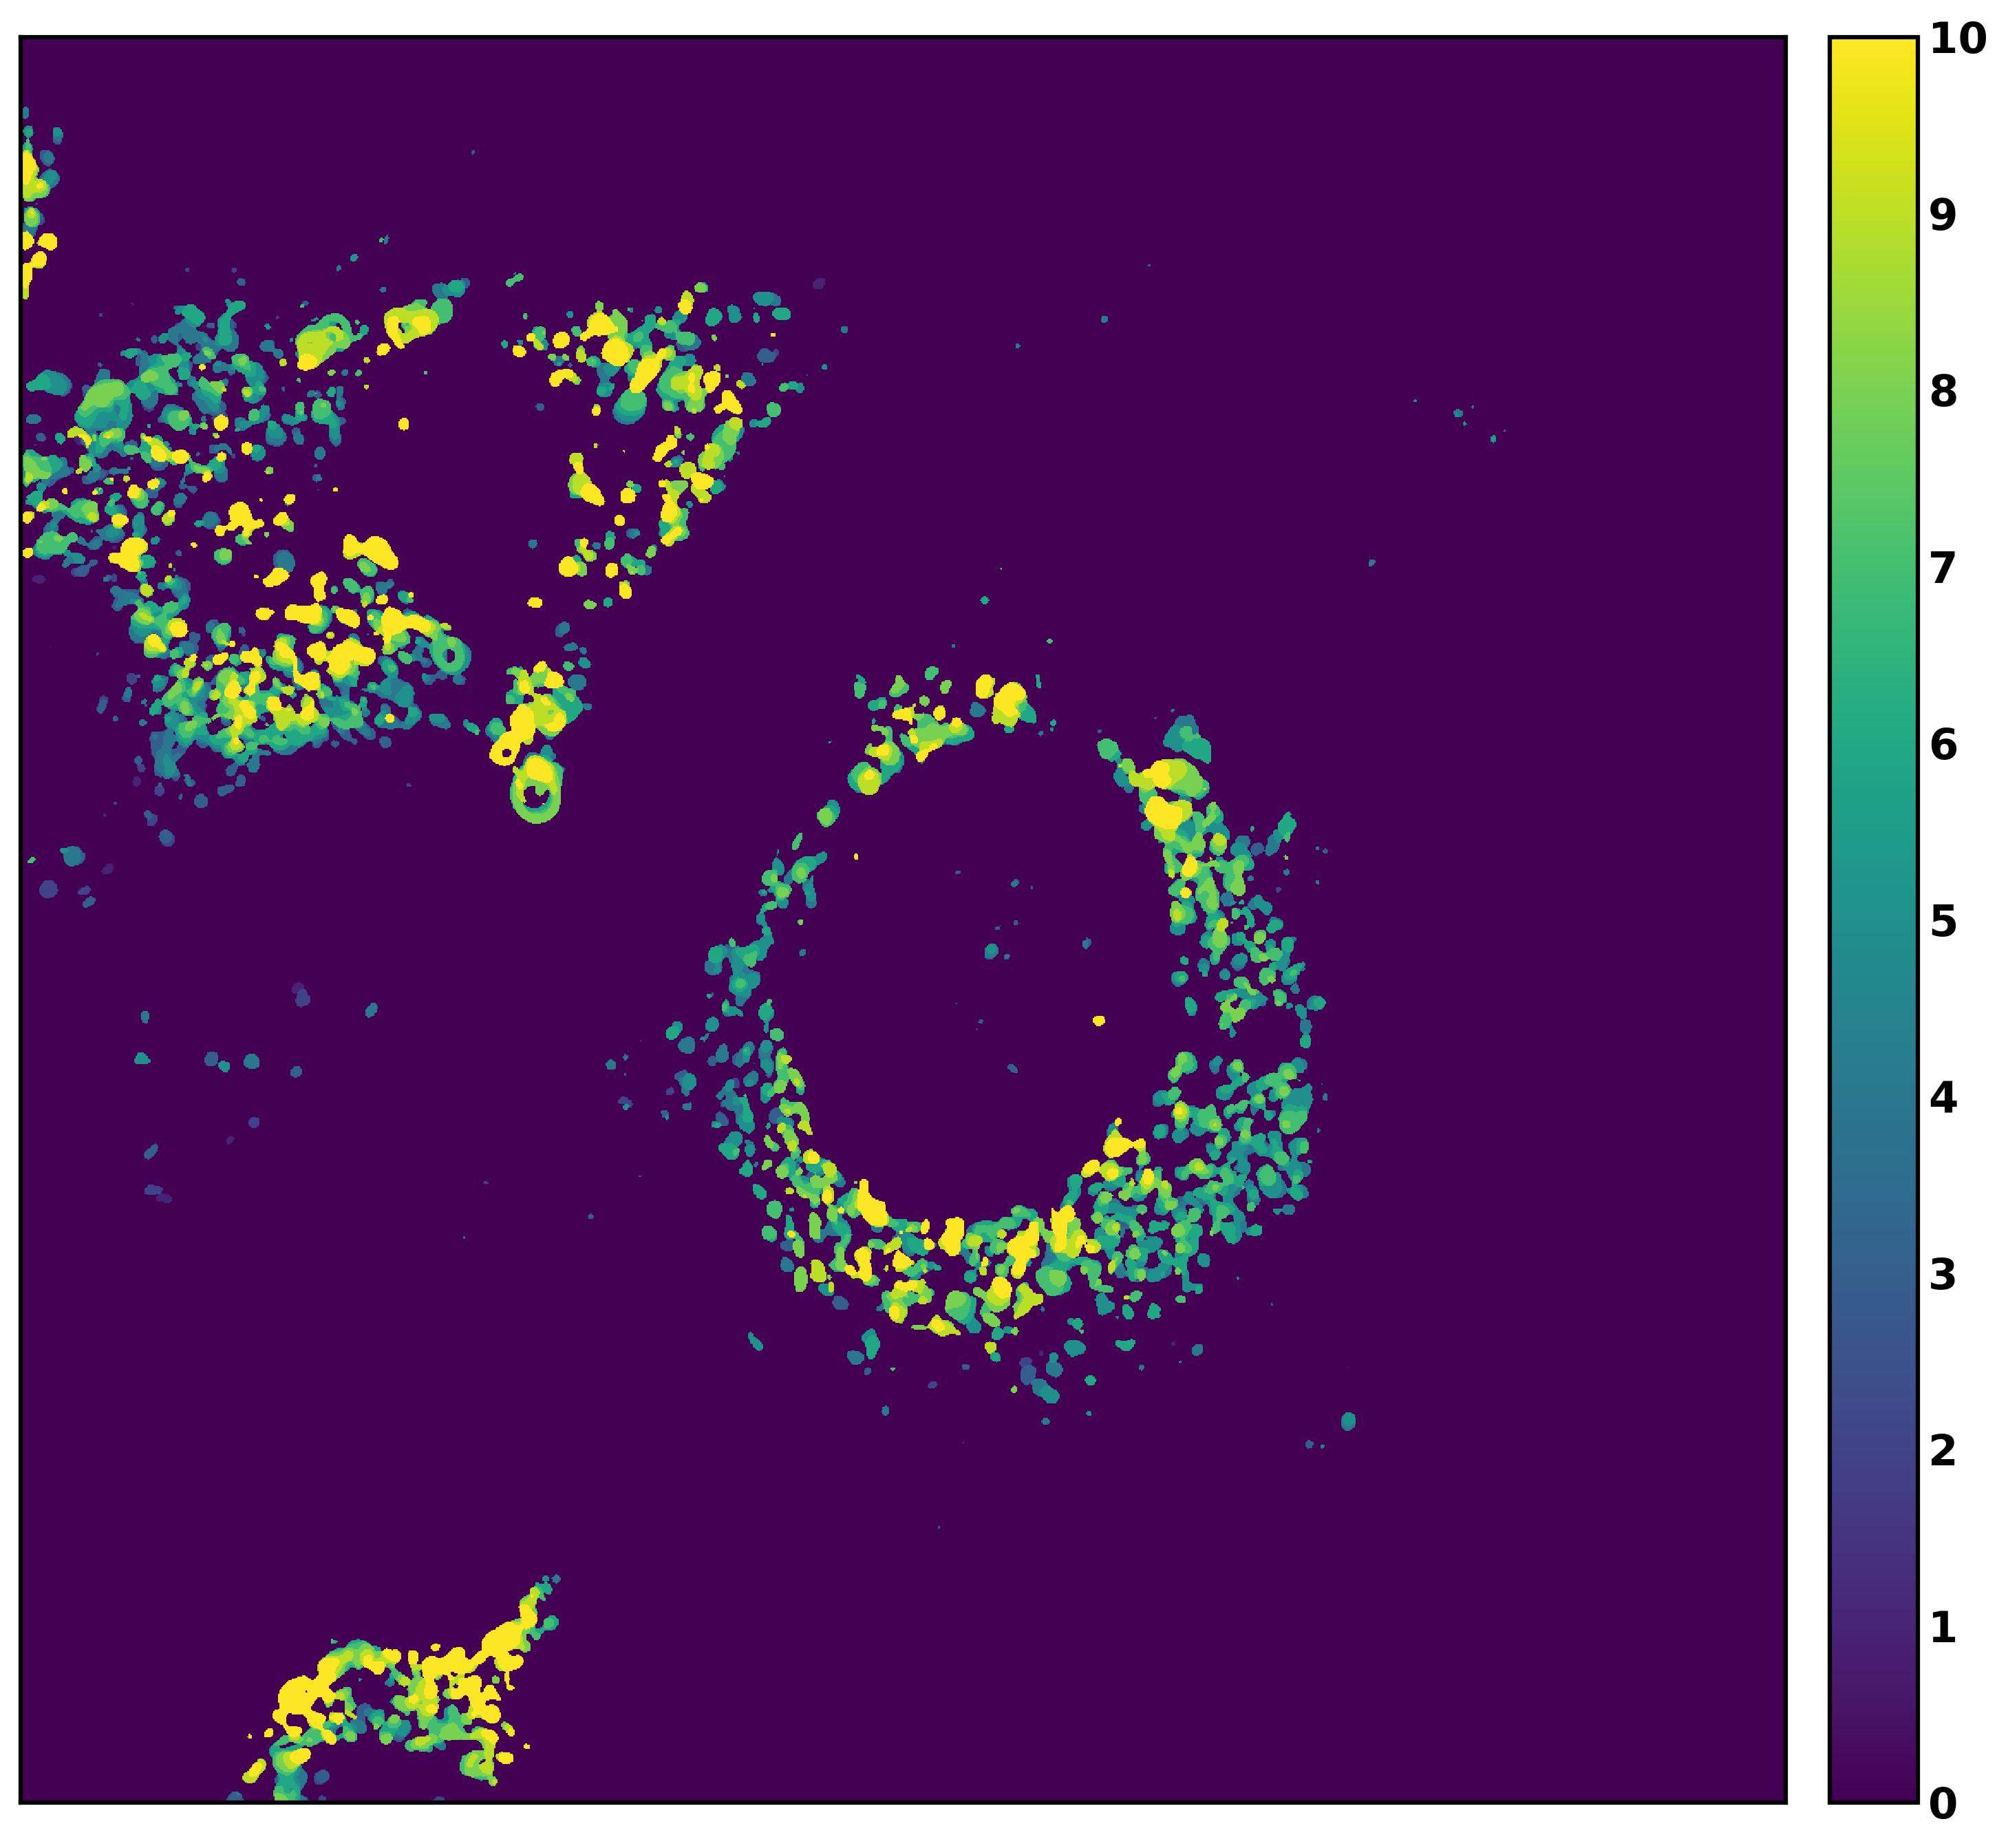
\includegraphics[width=0.32\textwidth]{figs/ch4figs/visual_analysis/global_outcomes/lyso/Flat_LML_4C=0_IsoData.png}}
	
	\caption[Showcase of the IsoData threshold outcomes with respect to the manual Hysteresis outcomes.]{Showcase of the IsoData thresholds outcomes with the top row being red-green overlay images with the IsoData outcomes in red, the Hysteresis thresholding outcomes in green, and overlaps of both outcomes in yellow. The bottom row showcases only the IsoData thresholding outcomes for improved clarity.}
	\label{fig:lyso_isodata}
\end{figure}
\FloatBarrier
\paragraph{Otsu} The showcase of the Otsu threshold outcomes is shown in Figure \ref{fig:lyso_otsu} with the Otsu threshold outcomes compared against the Hysteresis threshold outcomes in a red-green image for each sample. There are also binarized images for each sample of only the Otsu threshold outcomes which matches the red colour channel in the red-green images.
For sample A it is observed that the thresholding outcomes for both Otsu and Hysteresis thresholding are similar with an arguably negligible number of extra structures present in the Otsu threshold outcome but not at a scale that could imply under-thresholding. Given the greater presence of noise in sample A than in the other samples this could imply that Otsu has some noise resilience but this might be dependent on the presence of high average intensities for foreground structures. Sample B presents structures with greater volume than in the Hysteresis threshold outcomes resulting in the increased joining of structures. While the lower average structural intensities in sample B reduces the definition of structure edges this is still quite problematic and shows that Otsu might be too lenient for lower contrast structures. Sample C presents a few extra structures for the Otsu thresholding but with some of these foreground labelled structures being quite dim, compared relative to the other structure intensities, there may be a minor degree of noise or artefacts being incorrectly labelled as foreground.
\begin{figure}[h!]
	\subcaptionbox{Sample A overlayed}{\includegraphics[width=0.32\textwidth]{figs/ch4figs/visual_analysis/global_outcomes/lyso/Otsu_Con_2C=0.png}}
	\subcaptionbox{Sample B overlayed}{\includegraphics[width=0.32\textwidth]{figs/ch4figs/visual_analysis/global_outcomes/lyso/Otsu_LML_3C=0.png}}
	\subcaptionbox{Sample C overlayed}{\includegraphics[width=0.32\textwidth]{figs/ch4figs/visual_analysis/global_outcomes/lyso/Otsu_LML_4C=0.png}}
	
	\subcaptionbox{Sample A Otsu only}{\includegraphics[width=0.32\textwidth]{figs/ch4figs/visual_analysis/global_outcomes/lyso/Flat_Con_2C=0_Otsu.png}}
	\subcaptionbox{Sample B Otsu only}{\includegraphics[width=0.32\textwidth]{figs/ch4figs/visual_analysis/global_outcomes/lyso/Flat_LML_3C=0_Otsu.png}}
	\subcaptionbox{Sample C Otsu only}{\includegraphics[width=0.32\textwidth]{figs/ch4figs/visual_analysis/global_outcomes/lyso/Flat_LML_4C=0_Otsu.png}}
	
	\caption[Showcase of the Otsu threshold outcomes with respect to the manual Hysteresis outcomes.]{Showcase of the Otsu thresholds outcomes with the top row being red-green overlay images with the Otsu outcomes in red, the Hysteresis thresholding outcomes in green, and overlaps of both outcomes in yellow. The bottom row showcases only the Otsu thresholding outcomes for improved clarity.}
	\label{fig:lyso_otsu}
\end{figure}
\clearpage
\subsubsection{Local thresholding methods}
As there are only 4 local thresholding methods evaluated against only the top 2 performing methods will be explored further with these being the MidGrey and Bernsen thresold methods. An observation that can be made is that all of these thresholding outcomes are poor with all methods providing unusable results for sample A. This is likely due to the noise present in sample A being unfavourable to all of the local thresholding methods explored with performance varying for samples B and C.
\begin{table}[hb!]
	\centering
	\begin{tabular}{|c|c|c|c|c|}
		\hline
		\textbf{Method} & \textbf{Sample A} & \textbf{Sample B} & \textbf{Sample C} & \textbf{Mean Rank} \\
		\hline
		Bernsen & 1 & 3 & 2 & 2 \\
		\hline
		Mean & 1 & 2 & 2 & 1.6 \\
		\hline
		Median & 1 & 2 & 2 & 1.6 \\
		\hline
		MidGrey & 1 & 4 & 3 & 2.6 \\
		\hline
	\end{tabular}
	\caption{Rankings for each of the local thresholding methods for the lysosome sample images}
	\label{tab:lyso_local_ranks}
\end{table}
\FloatBarrier
\begin{figure}[h!]
	\subcaptionbox{Sample A overlayed}{\includegraphics[width=0.32\textwidth]{figs/ch4figs/visual_analysis/local_outcomes/lyso/MidGrey_Con_2C=0.png}}
	\subcaptionbox{Sample B overlayed}{\includegraphics[width=0.32\textwidth]{figs/ch4figs/visual_analysis/local_outcomes/lyso/MidGrey_LML_3C=0.png}}
	\subcaptionbox{Sample C overlayed}{\includegraphics[width=0.32\textwidth]{figs/ch4figs/visual_analysis/local_outcomes/lyso/MidGrey_LML_4C=0.png}}
	
	\subcaptionbox{Sample A MidGrey only}{\includegraphics[width=0.32\textwidth]{figs/ch4figs/visual_analysis/local_outcomes/lyso/Flat_Con_2C=0_MidGrey.png}}
	\subcaptionbox{Sample B MidGrey only}{\includegraphics[width=0.32\textwidth]{figs/ch4figs/visual_analysis/local_outcomes/lyso/Flat_LML_3C=0_MidGrey.png}}
	\subcaptionbox{Sample C MidGrey only}{\includegraphics[width=0.32\textwidth]{figs/ch4figs/visual_analysis/local_outcomes/lyso/Flat_LML_4C=0_MidGrey.png}}
	
	\caption[Showcase of the MidGrey threshold outcomes with respect to the manual Hysteresis outcomes.]{Showcase of the MidGrey thresholds outcomes with the top row being red-green overlay images with the MidGrey outcomes in red, the Hysteresis thresholding outcomes in green, and overlaps of both outcomes in yellow. The bottom row showcases only the MidGrey thresholding outcomes for improved clarity.}
	\label{fig:lyso_midgrey}
\end{figure}

\paragraph{MidGrey} The showcase of the MidGrey threshold outcomes is shown in Figure \ref{fig:lyso_midgrey} with the MidGrey threshold outcomes compared against the Hysteresis threshold outcomes in a red-green image for each sample. There are also binarized images for each sample of only the MidGrey threshold outcomes which matches the red colour channel in the red-green images. Sample B for MidGrey is a relatively good outcome that is similar to the Hysteresis thresholding outcome, with a minor quantity of foreground structures which are subjectively viable depending on the evaluator's bias, and without any extra structure joining that is not present in the Hysteresis thresholding outcome. For sample C there are more foreground structures compared to the Hysteresis thresholding outcome that do not all map to structures with intensities closer to the foreground than the background thus there is some measure, although minor, of under-thresholding occurring.

\FloatBarrier

\paragraph{Bernsen} The showcase of the Bernsen threshold outcomes is shown in Figure \ref{fig:lyso_bernsen} with the Bernsen threshold outcomes compared against the Hysteresis threshold outcomes in a red-green image for each sample. For sample B, while the primary foreground structures are the same as for the Hysteresis threshold outcome there is both an increased quantity of foreground structures and of structure joining. This makes the sample B outcome significantly less viable but minimal noise captured in the foreground renders this a weak but not wholly unusable result depending on the analysis. For sample C, there is an increase in the quantity of foreground structures, beyond what could be subjectively considered likely foreground, but there is an increase in structure separation. While not a great method for lysosome samples it could be applied for certain samples under specific image conditions but there are likely better methods to use.

\begin{figure}[h!]
	\subcaptionbox{Sample A overlayed}{\includegraphics[width=0.32\textwidth]{figs/ch4figs/visual_analysis/local_outcomes/lyso/Bernsen_Con_2C=0.png}}
	\subcaptionbox{Sample B overlayed}{\includegraphics[width=0.32\textwidth]{figs/ch4figs/visual_analysis/local_outcomes/lyso/Bernsen_LML_3C=0.png}}
	\subcaptionbox{Sample C overlayed}{\includegraphics[width=0.32\textwidth]{figs/ch4figs/visual_analysis/local_outcomes/lyso/Bernsen_LML_4C=0.png}}
	
	\subcaptionbox{Sample A Bernsen only}{\includegraphics[width=0.32\textwidth]{figs/ch4figs/visual_analysis/local_outcomes/lyso/Flat_Con_2C=0_Bernsen.png}}
	\subcaptionbox{Sample B Bernsen only}{\includegraphics[width=0.32\textwidth]{figs/ch4figs/visual_analysis/local_outcomes/lyso/Flat_LML_3C=0_Bernsen.png}}
	\subcaptionbox{Sample C Bernsen only}{\includegraphics[width=0.32\textwidth]{figs/ch4figs/visual_analysis/local_outcomes/lyso/Flat_LML_4C=0_Bernsen.png}}
	
	\caption[Showcase of the Bernsen threshold outcomes with respect to the manual Hysteresis outcomes.]{Showcase of the Bernsen thresholds outcomes with the top row being red-green overlay images with the Bernsen outcomes in red, the Hysteresis thresholding outcomes in green, and overlaps of both outcomes in yellow. The bottom row showcases only the Bernsen thresholding outcomes for improved clarity.}
	\label{fig:lyso_bernsen}
\end{figure}

\FloatBarrier
\subsubsection{AHT method with varied bias applications}
The rankings of the different AHT method biases are shown in Table \ref{tab:lyso_aht} with most of these methods presenting mediocre performance overall. It was observed that a consistent detractor to their performance was due to the AHT approximated low threshold being low enough that it induced excessive structure joining. 
\begin{table}
	\centering
	\begin{tabular}{|c|c|c|c|c|c|}
		\hline
		IHH bias applied & Window bias applied & Sample A & Sample B & Sample C & Mean Rank \\
		\hline
		No & None & 3 & 1 & 4 & 2.6 \\
		\hline
		No & Window width & 2 & 2 & 4 & 2.6 \\
		\hline
		No & Window mass & 2 & 1 & 4 & 2.3 \\
		\hline
		Yes & None & 2 & 3 & 4 & 3 \\
		\hline
		Yes & Window width & 2 & 3 & 3 & 2.6 \\
		\hline
		Yes & Window mass & 2 & 3 & 3 & 2.6 \\
		\hline
	\end{tabular}
	\caption{Rankings of the AHT threshold outcomes for the three samples with different combinations of the IHH and Window biases}
	\label{tab:lyso_aht}
\end{table}
\textcolor{red}{This is as far as I am currently. The current idea for the AHT is that since there isn't a clear top 3 I am considering taking the best, worst, and in-between? I am a bit uncertain. I am going to place three lineplots for the each of the lysosome samples which will have the IHH distribution, the inverted gradient distribution, vertical lines for the high threshold determined for each of the bias combos and potentially the distribution product (for when the IHH distribution is applied to the inverted gradient distribution). I plan to copy past this structure for autophagosomes and mitochondria.}

\FloatBarrier

\subsection{Autophagosome structures}
The autophagosome structure images are presented in Figure \ref{fig:autophagosome_raw} where the original MIP intensity images are shown along with the binary Hysteresis images for each sample. For each of these sample images, the accompanying Hysteresis threshold images are the foreground structures approximated through manual parameter tuning. \paragraph{Sample A:} Showcases foreground structures with high intensities that strongly contrast against the background but said background contains a large quantity of non-zero intensity noise and artefacts that could disrupt certain methods. \paragraph{Sample B:} Showcases foreground structures against a background containing little to no noise and, despite the maximum intensities for the majority of these structures being less than that of Sample A, the high contrast due to the low presence of noise could be ideal for many thresholding methods.\paragraph{Sample C:} Balanced between Sample A and Sample B, this sample possesses relatively high intensities for the foreground structures but with the presence of overlapping lower-intensity structure volumes, either belonging to out-of-focus structures or the structural volumes with low fluorophore concentrations, presents a challenge for confident differentiation for both manual and automatic thresholding methods.

\begin{figure}[ht!]
	\subcaptionbox{Sample A in Viridis}{\includegraphics[width=0.32\textwidth]{figs/ch4figs/visual_analysis/raw_samples/MAX_Con_2C=1.png}}
	\subcaptionbox{Sample B in Viridis}{\includegraphics[width=0.32\textwidth]{figs/ch4figs/visual_analysis/raw_samples/MAX_LML_3C=1.png}}
	\subcaptionbox{Sample C in Viridis}{\includegraphics[width=0.32\textwidth]{figs/ch4figs/visual_analysis/raw_samples/MAX_LML_4C=1.png}}
	\subcaptionbox{Sample A Hysteresis thresholding}{\includegraphics[width=0.32\textwidth]{figs/ch4figs/visual_analysis/raw_samples/Hyst_Con_2C=1.png}}
	\subcaptionbox{Sample B Hysteresis thresholding}{\includegraphics[width=0.32\textwidth]{figs/ch4figs/visual_analysis/raw_samples/Hyst_LML_3C=1.png}}
	\subcaptionbox{Sample C Hysteresis thresholding}{\includegraphics[width=0.32\textwidth]{figs/ch4figs/visual_analysis/raw_samples/Hyst_LML_4C=1.png}}
	\caption[Showcase of the autophagosome evaluation samples as MIP images.]{Showcase of the autophagosome evaluation samples as MIP images. The first row shows the pre-processed images, prior to any thresholding, in the viridis colourmap. The second row shows the same samples after manually tuned Hysteresis thresholding has been applied.}
	\label{fig:autophagosome_raw}
\end{figure}

\FloatBarrier
\subsubsection{Global thresholding methods}
For the autophagosome structures the top three global thresholding methods are Moments, IsoData and Otsu based on the mean rankings in Table \ref{tab:auto_global_ranks}.
\begin{table}[hb!]
	\centering
	\begin{tabular}{|c|c|c|c|c|}
		\hline
		\textbf{Method} & \textbf{Sample A} & \textbf{Sample B} & \textbf{Sample C} & \textbf{Mean Rank} \\
		\hline
		Huang2 & 1 & 2 & 2 & 1.6 \\
		\hline
		IsoData & 4 & 3 & 3 & 3.3 \\
		\hline
		Li & 1 & 1 & 1 & 1 \\
		\hline
		MaxEntropy & 1 & 3 & 2 & 2 \\
		\hline
		Moments & 3 & 3 & 5 & 3.6 \\
		\hline
		Otsu & 4 & 3 & 3 & 3.3 \\
		\hline
		RenyiEntropy & 1 & 3 & 5 & 3 \\
		\hline
		Triangle & 1 & 2 & 2 & 1.6 \\
		\hline
		Yen & 1 & 3 & 5 & 3 \\
		\hline
	\end{tabular}
	\caption{Rankings for each of the global thresholding methods for the autophagosome sample images}
	\label{tab:auto_global_ranks}
\end{table}

\FloatBarrier
\paragraph{Moments}
The showcase of the Moments threshold outcomes is shown in Figure \ref{fig:auto_moments} with the Moments threshold outcomes compared against the Hysteresis threshold outcomes in a red-green image for each sample. There are also binarized images for each sample of only the Moments threshold outcomes which matches the red colour channel in the red-green images. From this figure, it is observed that the Moments threshold and Hysteresis threshold outcomes for both samples A and B are very similar save for Moments having a few more foreground structures. Considering the greater low-intensity noise present in sample A, compared to the other samples, and the low average structural intensities for sample B this difference of a few structures is negligible since the Hysteresis thresholding baseline compared against is an imperfect ground truth due to the bias involved in it. The biggest deviation is for sample C where Moments separates structures that are joined in the Hysteresis threshold outcome but this joining is likely false, a flaw of Hysteresis thresholding, based on the intensity image of sample C in Figure \ref{fig:autophagosome_raw}. For this reason, it is deemed that Moments thresholding outperforms Hysteresis thresholding for sample C.
\begin{figure}[h!]
	\subcaptionbox{Sample A overlay}{\includegraphics[width=0.32\textwidth]{figs/ch4figs/visual_analysis/global_outcomes/auto/Moments_Con_2C=1.png}}
	\subcaptionbox{Sample B overlay}{\includegraphics[width=0.32\textwidth]{figs/ch4figs/visual_analysis/global_outcomes/auto/Moments_LML_3C=1.png}}
	\subcaptionbox{Sample C overlay}{\includegraphics[width=0.32\textwidth]{figs/ch4figs/visual_analysis/global_outcomes/auto/Moments_LML_4C=1.png}}
	
	\subcaptionbox{Sample A Moments only}{\includegraphics[width=0.32\textwidth]{figs/ch4figs/visual_analysis/global_outcomes/auto/Flat_Con_2C=1_Moments.png}}
	\subcaptionbox{Sample B Moments only}{\includegraphics[width=0.32\textwidth]{figs/ch4figs/visual_analysis/global_outcomes/auto/Flat_LML_3C=1_Moments.png}}
	\subcaptionbox{Sample C Moments only}{\includegraphics[width=0.32\textwidth]{figs/ch4figs/visual_analysis/global_outcomes/auto/Flat_LML_4C=1_Moments.png}}
	
	\caption[Showcase of the Moments threshold outcomes with respect to the manual Hysteresis outcomes.]{Showcase of the Moments thresholds outcomes with the top row being red-green overlay images with the Moments outcomes in red, the Hysteresis thresholding outcomes in green, and overlaps of both outcomes in yellow. The bottom row showcases only the Moments thresholding outcomes for improved clarity.}
	\label{fig:auto_moments}
\end{figure}

\FloatBarrier
\paragraph{IsoData} The showcase of the IsoData threshold outcomes is shown in Figure \ref{fig:auto_isodata} with the IsoData threshold outcomes compared against the Hysteresis threshold outcomes in a red-green image for each sample. There are also binarized images for each sample of only the IsoData threshold outcomes which matches the red colour channel in the red-green images. The IsoData outcomes for all of the autophagosome samples are quite similar to the Hysteresis thresholding outcomes although each expresses a minor degree of under-thresholding. This is observed to be a highly effective autosome structure thresholding method as the extra structures captured by IsoData, that are not present in the Hysteresis threshold outcomes, are for structures with a mean intensity closer to the Hysteresis thresholding labelled foreground structures than the background.

\begin{figure}[h!]
	\subcaptionbox{Sample A overlayed}{\includegraphics[width=0.32\textwidth]{figs/ch4figs/visual_analysis/global_outcomes/auto/IsoData_Con_2C=1.png}}
	\subcaptionbox{Sample B overlayed}{\includegraphics[width=0.32\textwidth]{figs/ch4figs/visual_analysis/global_outcomes/auto/IsoData_LML_3C=1.png}}
	\subcaptionbox{Sample C overlayed}{\includegraphics[width=0.32\textwidth]{figs/ch4figs/visual_analysis/global_outcomes/auto/IsoData_LML_4C=1.png}}
	
	\subcaptionbox{Sample A IsoData only}{\includegraphics[width=0.32\textwidth]{figs/ch4figs/visual_analysis/global_outcomes/auto/Flat_Con_2C=1_IsoData.png}}
	\subcaptionbox{Sample B IsoData only}{\includegraphics[width=0.32\textwidth]{figs/ch4figs/visual_analysis/global_outcomes/auto/Flat_LML_3C=1_IsoData.png}}
	\subcaptionbox{Sample C IsoData only}{\includegraphics[width=0.32\textwidth]{figs/ch4figs/visual_analysis/global_outcomes/auto/Flat_LML_4C=1_IsoData.png}}
	
	\caption[Showcase of the IsoData threshold outcomes with respect to the manual Hysteresis outcomes.]{Showcase of the IsoData thresholds outcomes with the top row being red-green overlay images with the IsoData outcomes in red, the Hysteresis thresholding outcomes in green, and overlaps of both outcomes in yellow. The bottom row showcases only the IsoData thresholding outcomes for improved clarity.}
	\label{fig:auto_isodata}
\end{figure}
\FloatBarrier
\paragraph{Otsu} The showcase of the Otsu threshold outcomes is shown in Figure \ref{fig:auto_otsu} with the Otsu threshold outcomes compared against the Hysteresis threshold outcomes in a red-green image for each sample. There are also binarized images for each sample of only the Otsu threshold outcomes which matches the red colour channel in the red-green images.
For sample A it is observed that the thresholding outcomes for both Otsu and Hysteresis thresholding are similar with an arguably negligible number of extra structures present in the Otsu threshold outcome but not at a scale that could imply under-thresholding. Given the greater presence of noise in sample A than in the other samples this could imply that Otsu has some noise resilience but this might be dependent on the presence of high average intensities for foreground structures. Sample B presents structures with greater volume than in the Hysteresis threshold outcomes resulting in the increased joining of structures. While the lower average structural intensities in sample B reduces the definition of structure edges this is still quite problematic and shows that Otsu might be too lenient for lower contrast structures. Sample C presents a few extra structures for the Otsu thresholding but with some of these foreground labelled structures being quite dim, compared relative to the other structure intensities, there may be a minor degree of noise or artefacts being incorrectly labelled as foreground.
\begin{figure}[h!]
	\subcaptionbox{Sample A overlayed}{\includegraphics[width=0.32\textwidth]{figs/ch4figs/visual_analysis/global_outcomes/auto/Otsu_Con_2C=1.png}}
	\subcaptionbox{Sample B overlayed}{\includegraphics[width=0.32\textwidth]{figs/ch4figs/visual_analysis/global_outcomes/auto/Otsu_LML_3C=1.png}}
	\subcaptionbox{Sample C overlayed}{\includegraphics[width=0.32\textwidth]{figs/ch4figs/visual_analysis/global_outcomes/auto/Otsu_LML_4C=1.png}}
	
	\subcaptionbox{Sample A Otsu only}{\includegraphics[width=0.32\textwidth]{figs/ch4figs/visual_analysis/global_outcomes/auto/Flat_Con_2C=1_Otsu.png}}
	\subcaptionbox{Sample B Otsu only}{\includegraphics[width=0.32\textwidth]{figs/ch4figs/visual_analysis/global_outcomes/auto/Flat_LML_3C=1_Otsu.png}}
	\subcaptionbox{Sample C Otsu only}{\includegraphics[width=0.32\textwidth]{figs/ch4figs/visual_analysis/global_outcomes/auto/Flat_LML_4C=1_Otsu.png}}
	
	\caption[Showcase of the Otsu threshold outcomes with respect to the manual Hysteresis outcomes.]{Showcase of the Otsu thresholds outcomes with the top row being red-green overlay images with the Otsu outcomes in red, the Hysteresis thresholding outcomes in green, and overlaps of both outcomes in yellow. The bottom row showcases only the Otsu thresholding outcomes for improved clarity.}
	\label{fig:auto_otsu}
\end{figure}
\clearpage
\subsubsection{Local thresholding methods}
As there are only 4 local thresholding methods evaluated against only the top 2 performing methods will be explored further with these being the MidGrey and Bernsen thresold methods. An observation that can be made is that all of these thresholding outcomes are poor with all methods providing unusable results for sample A. This is likely due to the noise present in sample A being unfavourable to all of the local thresholding methods explored with performance varying for samples B and C.
\begin{table}[hb!]
	\centering
	\begin{tabular}{|c|c|c|c|c|}
		\hline
		\textbf{Method} & \textbf{Sample A} & \textbf{Sample B} & \textbf{Sample C} & \textbf{Mean Rank} \\
		\hline
		Bernsen & 1 & 3 & 2 & 2 \\
		\hline
		Mean & 1 & 2 & 2 & 1.6 \\
		\hline
		Median & 1 & 2 & 2 & 1.6 \\
		\hline
		MidGrey & 1 & 4 & 3 & 2.6 \\
		\hline
	\end{tabular}
	\caption{Rankings for each of the local thresholding methods for the autosome sample images}
	\label{tab:auto_local_ranks}
\end{table}
\FloatBarrier
\begin{figure}[h!]
	\subcaptionbox{Sample A overlayed}{\includegraphics[width=0.32\textwidth]{figs/ch4figs/visual_analysis/local_outcomes/auto/MidGrey_Con_2C=1.png}}
	\subcaptionbox{Sample B overlayed}{\includegraphics[width=0.32\textwidth]{figs/ch4figs/visual_analysis/local_outcomes/auto/MidGrey_LML_3C=1.png}}
	\subcaptionbox{Sample C overlayed}{\includegraphics[width=0.32\textwidth]{figs/ch4figs/visual_analysis/local_outcomes/auto/MidGrey_LML_4C=1.png}}
	
	\subcaptionbox{Sample A MidGrey only}{\includegraphics[width=0.32\textwidth]{figs/ch4figs/visual_analysis/local_outcomes/auto/Flat_Con_2C=1_MidGrey.png}}
	\subcaptionbox{Sample B MidGrey only}{\includegraphics[width=0.32\textwidth]{figs/ch4figs/visual_analysis/local_outcomes/auto/Flat_LML_3C=1_MidGrey.png}}
	\subcaptionbox{Sample C MidGrey only}{\includegraphics[width=0.32\textwidth]{figs/ch4figs/visual_analysis/local_outcomes/auto/Flat_LML_4C=1_MidGrey.png}}
	
	\caption[Showcase of the MidGrey threshold outcomes with respect to the manual Hysteresis outcomes.]{Showcase of the MidGrey thresholds outcomes with the top row being red-green overlay images with the MidGrey outcomes in red, the Hysteresis thresholding outcomes in green, and overlaps of both outcomes in yellow. The bottom row showcases only the MidGrey thresholding outcomes for improved clarity.}
	\label{fig:auto_midgrey}
\end{figure}

\paragraph{MidGrey} The showcase of the MidGrey threshold outcomes is shown in Figure \ref{fig:auto_midgrey} with the MidGrey threshold outcomes compared against the Hysteresis threshold outcomes in a red-green image for each sample. There are also binarized images for each sample of only the MidGrey threshold outcomes which matches the red colour channel in the red-green images. Sample B for MidGrey is a relatively good outcome that is similar to the Hysteresis thresholding outcome, with a minor quantity of foreground structures which are subjectively viable depending on the evaluator's bias, and without any extra structure joining that is not present in the Hysteresis thresholding outcome. For sample C there are more foreground structures compared to the Hysteresis thresholding outcome that do not all map to structures with intensities closer to the foreground than the background thus there is some measure, although minor, of under-thresholding occurring.

\FloatBarrier

\paragraph{Bernsen} The showcase of the Bernsen threshold outcomes is shown in Figure \ref{fig:auto_bernsen} with the Bernsen threshold outcomes compared against the Hysteresis threshold outcomes in a red-green image for each sample. For sample B, while the primary foreground structures are the same as for the Hysteresis threshold outcome there is both an increased quantity of foreground structures and of structure joining. This makes the sample B outcome significantly less viable but minimal noise captured in the foreground renders this a weak but not wholly unusable result depending on the analysis. For sample C, there is an increase in the quantity of foreground structures, beyond what could be subjectively considered likely foreground, but there is an increase in structure separation. While not a great method for autosome samples it could be applied for certain samples under specific image conditions but there are likely better methods to use.

\begin{figure}[h!]
	\subcaptionbox{Sample A overlayed}{\includegraphics[width=0.32\textwidth]{figs/ch4figs/visual_analysis/local_outcomes/auto/Bernsen_Con_2C=1.png}}
	\subcaptionbox{Sample B overlayed}{\includegraphics[width=0.32\textwidth]{figs/ch4figs/visual_analysis/local_outcomes/auto/Bernsen_LML_3C=1.png}}
	\subcaptionbox{Sample C overlayed}{\includegraphics[width=0.32\textwidth]{figs/ch4figs/visual_analysis/local_outcomes/auto/Bernsen_LML_4C=1.png}}
	
	\subcaptionbox{Sample A Bernsen only}{\includegraphics[width=0.32\textwidth]{figs/ch4figs/visual_analysis/local_outcomes/auto/Flat_Con_2C=1_Bernsen.png}}
	\subcaptionbox{Sample B Bernsen only}{\includegraphics[width=0.32\textwidth]{figs/ch4figs/visual_analysis/local_outcomes/auto/Flat_LML_3C=1_Bernsen.png}}
	\subcaptionbox{Sample C Bernsen only}{\includegraphics[width=0.32\textwidth]{figs/ch4figs/visual_analysis/local_outcomes/auto/Flat_LML_4C=1_Bernsen.png}}
	
	\caption[Showcase of the Bernsen threshold outcomes with respect to the manual Hysteresis outcomes.]{Showcase of the Bernsen thresholds outcomes with the top row being red-green overlay images with the Bernsen outcomes in red, the Hysteresis thresholding outcomes in green, and overlaps of both outcomes in yellow. The bottom row showcases only the Bernsen thresholding outcomes for improved clarity.}
	\label{fig:auto_bernsen}
\end{figure}



